\documentclass[twoside]{book}

% Packages required by doxygen
\usepackage{fixltx2e}
\usepackage{calc}
\usepackage{doxygen}
\usepackage[export]{adjustbox} % also loads graphicx
\usepackage{graphicx}
\usepackage[utf8]{inputenc}
\usepackage{makeidx}
\usepackage{multicol}
\usepackage{multirow}
\PassOptionsToPackage{warn}{textcomp}
\usepackage{textcomp}
\usepackage[nointegrals]{wasysym}
\usepackage[table]{xcolor}

% Font selection
\usepackage[T1]{fontenc}
\usepackage[scaled=.90]{helvet}
\usepackage{courier}
\usepackage{amssymb}
\usepackage{sectsty}
\renewcommand{\familydefault}{\sfdefault}
\allsectionsfont{%
  \fontseries{bc}\selectfont%
  \color{darkgray}%
}
\renewcommand{\DoxyLabelFont}{%
  \fontseries{bc}\selectfont%
  \color{darkgray}%
}
\newcommand{\+}{\discretionary{\mbox{\scriptsize$\hookleftarrow$}}{}{}}

% Page & text layout
\usepackage{geometry}
\geometry{%
  a4paper,%
  top=2.5cm,%
  bottom=2.5cm,%
  left=2.5cm,%
  right=2.5cm%
}
\tolerance=750
\hfuzz=15pt
\hbadness=750
\setlength{\emergencystretch}{15pt}
\setlength{\parindent}{0cm}
\setlength{\parskip}{3ex plus 2ex minus 2ex}
\makeatletter
\renewcommand{\paragraph}{%
  \@startsection{paragraph}{4}{0ex}{-1.0ex}{1.0ex}{%
    \normalfont\normalsize\bfseries\SS@parafont%
  }%
}
\renewcommand{\subparagraph}{%
  \@startsection{subparagraph}{5}{0ex}{-1.0ex}{1.0ex}{%
    \normalfont\normalsize\bfseries\SS@subparafont%
  }%
}
\makeatother

% Headers & footers
\usepackage{fancyhdr}
\pagestyle{fancyplain}
\fancyhead[LE]{\fancyplain{}{\bfseries\thepage}}
\fancyhead[CE]{\fancyplain{}{}}
\fancyhead[RE]{\fancyplain{}{\bfseries\leftmark}}
\fancyhead[LO]{\fancyplain{}{\bfseries\rightmark}}
\fancyhead[CO]{\fancyplain{}{}}
\fancyhead[RO]{\fancyplain{}{\bfseries\thepage}}
\fancyfoot[LE]{\fancyplain{}{}}
\fancyfoot[CE]{\fancyplain{}{}}
\fancyfoot[RE]{\fancyplain{}{\bfseries\scriptsize Generated by Doxygen }}
\fancyfoot[LO]{\fancyplain{}{\bfseries\scriptsize Generated by Doxygen }}
\fancyfoot[CO]{\fancyplain{}{}}
\fancyfoot[RO]{\fancyplain{}{}}
\renewcommand{\footrulewidth}{0.4pt}
\renewcommand{\chaptermark}[1]{%
  \markboth{#1}{}%
}
\renewcommand{\sectionmark}[1]{%
  \markright{\thesection\ #1}%
}

% Indices & bibliography
\usepackage{natbib}
\usepackage[titles]{tocloft}
\setcounter{tocdepth}{3}
\setcounter{secnumdepth}{5}
\makeindex

% Hyperlinks (required, but should be loaded last)
\usepackage{ifpdf}
\ifpdf
  \usepackage[pdftex,pagebackref=true]{hyperref}
\else
  \usepackage[ps2pdf,pagebackref=true]{hyperref}
\fi
\hypersetup{%
  colorlinks=true,%
  linkcolor=blue,%
  citecolor=blue,%
  unicode%
}

% Custom commands
\newcommand{\clearemptydoublepage}{%
  \newpage{\pagestyle{empty}\cleardoublepage}%
}

\usepackage{caption}
\captionsetup{labelsep=space,justification=centering,font={bf},singlelinecheck=off,skip=4pt,position=top}

%===== C O N T E N T S =====

\begin{document}

% Titlepage & ToC
\hypersetup{pageanchor=false,
             bookmarksnumbered=true,
             pdfencoding=unicode
            }
\pagenumbering{alph}
\begin{titlepage}
\vspace*{7cm}
\begin{center}%
{\Large V\+EX 709S }\\
\vspace*{1cm}
{\large Generated by Doxygen 1.8.14}\\
\end{center}
\end{titlepage}
\clearemptydoublepage
\pagenumbering{roman}
\tableofcontents
\clearemptydoublepage
\pagenumbering{arabic}
\hypersetup{pageanchor=true}

%--- Begin generated contents ---
\chapter{V\+E\+X-\/709\+S-\/2018}
\label{md__home_ethan_VEX-709S-2018_README}
\Hypertarget{md__home_ethan_VEX-709S-2018_README}
Repository for V\+EX Robotics Competition team 709S for the 2017-\/2018 game 
\chapter{Namespace Index}
\section{Namespace List}
Here is a list of all documented namespaces with brief descriptions\+:\begin{DoxyCompactList}
\item\contentsline{section}{\hyperlink{namespacedebug}{debug} }{\pageref{namespacedebug}}{}
\item\contentsline{section}{\hyperlink{namespacedrive}{drive} }{\pageref{namespacedrive}}{}
\item\contentsline{section}{\hyperlink{namespacedrive_1_1accel}{drive\+::accel} }{\pageref{namespacedrive_1_1accel}}{}
\item\contentsline{section}{\hyperlink{namespacelift}{lift} }{\pageref{namespacelift}}{}
\item\contentsline{section}{\hyperlink{namespacemotors}{motors} }{\pageref{namespacemotors}}{}
\item\contentsline{section}{\hyperlink{namespacemotors_1_1slew}{motors\+::slew} }{\pageref{namespacemotors_1_1slew}}{}
\item\contentsline{section}{\hyperlink{namespacepid}{pid} }{\pageref{namespacepid}}{}
\item\contentsline{section}{\hyperlink{namespacesensors}{sensors} }{\pageref{namespacesensors}}{}
\end{DoxyCompactList}

\chapter{Hierarchical Index}
\section{Class Hierarchy}
This inheritance list is sorted roughly, but not completely, alphabetically\+:\begin{DoxyCompactList}
\item \contentsline{section}{sensors\+:\+:button\+\_\+t}{\pageref{structsensors_1_1button__t}}{}
\item \contentsline{section}{gyro\+:\+:drive}{\pageref{classgyro_1_1drive}}{}
\item \contentsline{section}{sensors\+:\+:gyro\+\_\+t}{\pageref{classsensors_1_1gyro__t}}{}
\item \contentsline{section}{motor\+\_\+t}{\pageref{structmotor__t}}{}
\item object\begin{DoxyCompactList}
\item \contentsline{section}{commit.\+Commit}{\pageref{classcommit_1_1Commit}}{}
\end{DoxyCompactList}
\item \contentsline{section}{sensors\+:\+:pot\+\_\+t}{\pageref{structsensors_1_1pot__t}}{}
\item \contentsline{section}{sensors\+:\+:quad\+\_\+t}{\pageref{structsensors_1_1quad__t}}{}
\item \contentsline{section}{drive\+:\+:side\+\_\+t}{\pageref{structdrive_1_1side__t}}{}
\item \contentsline{section}{lift\+:\+:side\+\_\+t}{\pageref{structlift_1_1side__t}}{}
\item \contentsline{section}{sensors\+:\+:sonic\+\_\+t}{\pageref{structsensors_1_1sonic__t}}{}
\end{DoxyCompactList}

\chapter{Class Index}
\section{Class List}
Here are the classes, structs, unions and interfaces with brief descriptions\+:\begin{DoxyCompactList}
\item\contentsline{section}{\hyperlink{structsensors_1_1button__t}{sensors\+::button\+\_\+t} }{\pageref{structsensors_1_1button__t}}{}
\item\contentsline{section}{\hyperlink{classgyro_1_1drive}{gyro\+::drive} }{\pageref{classgyro_1_1drive}}{}
\item\contentsline{section}{\hyperlink{classsensors_1_1gyro__t}{sensors\+::gyro\+\_\+t} }{\pageref{classsensors_1_1gyro__t}}{}
\item\contentsline{section}{\hyperlink{structmotor__t}{motor\+\_\+t} }{\pageref{structmotor__t}}{}
\item\contentsline{section}{\hyperlink{structsensors_1_1pot__t}{sensors\+::pot\+\_\+t} }{\pageref{structsensors_1_1pot__t}}{}
\item\contentsline{section}{\hyperlink{structsensors_1_1quad__t}{sensors\+::quad\+\_\+t} }{\pageref{structsensors_1_1quad__t}}{}
\item\contentsline{section}{\hyperlink{structdrive_1_1side__t}{drive\+::side\+\_\+t} }{\pageref{structdrive_1_1side__t}}{}
\item\contentsline{section}{\hyperlink{structlift_1_1side__t}{lift\+::side\+\_\+t} }{\pageref{structlift_1_1side__t}}{}
\item\contentsline{section}{\hyperlink{structsensors_1_1sonic__t}{sensors\+::sonic\+\_\+t} }{\pageref{structsensors_1_1sonic__t}}{}
\end{DoxyCompactList}

\chapter{File Index}
\section{File List}
Here is a list of all documented files with brief descriptions\+:\begin{DoxyCompactList}
\item\contentsline{section}{include/\hyperlink{API_8h}{A\+P\+I.\+h} \\*Provides the high-\/level user functionality intended for use by typical V\+EX Cortex programmers }{\pageref{API_8h}}{}
\item\contentsline{section}{include/{\bfseries debug.\+hpp} }{\pageref{debug_8hpp}}{}
\item\contentsline{section}{include/{\bfseries drive.\+hpp} }{\pageref{drive_8hpp}}{}
\item\contentsline{section}{include/{\bfseries gyro.\+hpp} }{\pageref{gyro_8hpp}}{}
\item\contentsline{section}{include/{\bfseries lift.\+hpp} }{\pageref{lift_8hpp}}{}
\item\contentsline{section}{include/\hyperlink{main_8h}{main.\+h} \\*Header file for global functions }{\pageref{main_8h}}{}
\item\contentsline{section}{include/{\bfseries motors.\+hpp} }{\pageref{motors_8hpp}}{}
\item\contentsline{section}{include/{\bfseries pid.\+hpp} }{\pageref{pid_8hpp}}{}
\item\contentsline{section}{include/{\bfseries sensors.\+hpp} }{\pageref{sensors_8hpp}}{}
\end{DoxyCompactList}

\chapter{Namespace Documentation}
\hypertarget{namespacedebug}{}\section{debug Namespace Reference}
\label{namespacedebug}\index{debug@{debug}}
\subsection*{Functions}
\begin{DoxyCompactItemize}
\item 
void \hyperlink{namespacedebug_a1b083c25ffa805221c19f97c56351855}{debug} (void)
\end{DoxyCompactItemize}
\subsection*{Variables}
\begin{DoxyCompactItemize}
\item 
\mbox{\Hypertarget{namespacedebug_a507b3f8f70ba072d22b18ab9c8e074f4}\label{namespacedebug_a507b3f8f70ba072d22b18ab9c8e074f4}} 
uint32\+\_\+t {\bfseries fault} = 0
\end{DoxyCompactItemize}


\subsection{Detailed Description}
Contains debugging funtions, etc 

\subsection{Function Documentation}
\mbox{\Hypertarget{namespacedebug_a1b083c25ffa805221c19f97c56351855}\label{namespacedebug_a1b083c25ffa805221c19f97c56351855}} 
\index{debug@{debug}!debug@{debug}}
\index{debug@{debug}!debug@{debug}}
\subsubsection{\texorpdfstring{debug()}{debug()}}
{\footnotesize\ttfamily void debug\+::debug (\begin{DoxyParamCaption}\item[{void}]{ }\end{DoxyParamCaption})}

Debug the Cortex if something goes wrong 
\hypertarget{namespacedrive}{}\section{drive Namespace Reference}
\label{namespacedrive}\index{drive@{drive}}
\subsection*{Namespaces}
\begin{DoxyCompactItemize}
\item 
 \hyperlink{namespacedrive_1_1accel}{accel}
\end{DoxyCompactItemize}
\subsection*{Classes}
\begin{DoxyCompactItemize}
\item 
struct \hyperlink{structdrive_1_1side__t}{side\+\_\+t}
\end{DoxyCompactItemize}
\subsection*{Functions}
\begin{DoxyCompactItemize}
\item 
void \hyperlink{namespacedrive_a2df65772c3853804f68f3358b04420b2}{set} (int lpower, int rpower)
\item 
void \hyperlink{namespacedrive_afb11be06c88e18373ad210a65e146d53}{init} (void)
\item 
void \hyperlink{namespacedrive_ab1c99e0f944b404b036034bac0074ca6}{inches} (long inches)
\item 
void \hyperlink{namespacedrive_a4468fd8982ce72051c07b37cf1f91185}{tank} (void)
\end{DoxyCompactItemize}
\subsection*{Variables}
\begin{DoxyCompactItemize}
\item 
double \hyperlink{namespacedrive_ac57641567511fcbc0ce6bf72b1aff76e}{inch}
\item 
\hyperlink{structdrive_1_1side__t}{side\+\_\+t} \hyperlink{namespacedrive_abde1df4410c0d0bfc462f3fb33ab9c5d}{left}
\item 
\hyperlink{structdrive_1_1side__t}{side\+\_\+t} \hyperlink{namespacedrive_a6adcb98f34f373f5e1fae1c46b8d7269}{right}
\end{DoxyCompactItemize}


\subsection{Detailed Description}
Contains everything relating to the drive 

\subsection{Function Documentation}
\mbox{\Hypertarget{namespacedrive_ab1c99e0f944b404b036034bac0074ca6}\label{namespacedrive_ab1c99e0f944b404b036034bac0074ca6}} 
\index{drive@{drive}!inches@{inches}}
\index{inches@{inches}!drive@{drive}}
\subsubsection{\texorpdfstring{inches()}{inches()}}
{\footnotesize\ttfamily void drive\+::inches (\begin{DoxyParamCaption}\item[{long}]{inches }\end{DoxyParamCaption})}

Drive a specific number of inches \mbox{\Hypertarget{namespacedrive_afb11be06c88e18373ad210a65e146d53}\label{namespacedrive_afb11be06c88e18373ad210a65e146d53}} 
\index{drive@{drive}!init@{init}}
\index{init@{init}!drive@{drive}}
\subsubsection{\texorpdfstring{init()}{init()}}
{\footnotesize\ttfamily void drive\+::init (\begin{DoxyParamCaption}\item[{void}]{ }\end{DoxyParamCaption})}

Initialize the drive subsystem \mbox{\Hypertarget{namespacedrive_a2df65772c3853804f68f3358b04420b2}\label{namespacedrive_a2df65772c3853804f68f3358b04420b2}} 
\index{drive@{drive}!set@{set}}
\index{set@{set}!drive@{drive}}
\subsubsection{\texorpdfstring{set()}{set()}}
{\footnotesize\ttfamily void drive\+::set (\begin{DoxyParamCaption}\item[{int}]{lpower,  }\item[{int}]{rpower }\end{DoxyParamCaption})}

Set both sides of the drive at their requested powers \mbox{\Hypertarget{namespacedrive_a4468fd8982ce72051c07b37cf1f91185}\label{namespacedrive_a4468fd8982ce72051c07b37cf1f91185}} 
\index{drive@{drive}!tank@{tank}}
\index{tank@{tank}!drive@{drive}}
\subsubsection{\texorpdfstring{tank()}{tank()}}
{\footnotesize\ttfamily void drive\+::tank (\begin{DoxyParamCaption}\item[{void}]{ }\end{DoxyParamCaption})}

Tank control that should be used in a while loop 

\subsection{Variable Documentation}
\mbox{\Hypertarget{namespacedrive_ac57641567511fcbc0ce6bf72b1aff76e}\label{namespacedrive_ac57641567511fcbc0ce6bf72b1aff76e}} 
\index{drive@{drive}!inch@{inch}}
\index{inch@{inch}!drive@{drive}}
\subsubsection{\texorpdfstring{inch}{inch}}
{\footnotesize\ttfamily double drive\+::inch}

{\bfseries Initial value\+:}
\begin{DoxyCode}
=
      28.64788975654116043839907740705258516620273623328216077458012735
\end{DoxyCode}
Multiplier for which 1 inch is used to convert into degreees rotation on 4" wheels \mbox{\Hypertarget{namespacedrive_abde1df4410c0d0bfc462f3fb33ab9c5d}\label{namespacedrive_abde1df4410c0d0bfc462f3fb33ab9c5d}} 
\index{drive@{drive}!left@{left}}
\index{left@{left}!drive@{drive}}
\subsubsection{\texorpdfstring{left}{left}}
{\footnotesize\ttfamily \hyperlink{structdrive_1_1side__t}{side\+\_\+t} drive\+::left}

The left side of the drive \mbox{\Hypertarget{namespacedrive_a6adcb98f34f373f5e1fae1c46b8d7269}\label{namespacedrive_a6adcb98f34f373f5e1fae1c46b8d7269}} 
\index{drive@{drive}!right@{right}}
\index{right@{right}!drive@{drive}}
\subsubsection{\texorpdfstring{right}{right}}
{\footnotesize\ttfamily \hyperlink{structdrive_1_1side__t}{side\+\_\+t} drive\+::right}

The right side of the drive 
\hypertarget{namespacedrive_1_1accel}{}\section{drive\+:\+:accel Namespace Reference}
\label{namespacedrive_1_1accel}\index{drive\+::accel@{drive\+::accel}}
\subsection*{Functions}
\begin{DoxyCompactItemize}
\item 
void \hyperlink{namespacedrive_1_1accel_a6d0c42c5e3f1ff1db68617de9d4b1758}{drive} (void)
\end{DoxyCompactItemize}
\subsection*{Variables}
\begin{DoxyCompactItemize}
\item 
int \hyperlink{namespacedrive_1_1accel_ac04cdc79ef60e183664808e63c64204a}{x} = 0
\item 
int \hyperlink{namespacedrive_1_1accel_ab30da3026058091c6ee42e12c4e62432}{y} = 0
\item 
int \hyperlink{namespacedrive_1_1accel_aff072ce199309a54b7bc8e3f80f6e15c}{prevX} = 0
\item 
int \hyperlink{namespacedrive_1_1accel_ae0f4ef2b1c049d481f496d680dd3f9bd}{prevY} = 0
\item 
\mbox{\Hypertarget{namespacedrive_1_1accel_a14bc27053dde38ad7e09e8bb78c44d1a}\label{namespacedrive_1_1accel_a14bc27053dde38ad7e09e8bb78c44d1a}} 
int {\bfseries deadband} = 20
\end{DoxyCompactItemize}


\subsection{Detailed Description}
Joystick accelerometer driving! 

\subsection{Function Documentation}
\mbox{\Hypertarget{namespacedrive_1_1accel_a6d0c42c5e3f1ff1db68617de9d4b1758}\label{namespacedrive_1_1accel_a6d0c42c5e3f1ff1db68617de9d4b1758}} 
\index{drive\+::accel@{drive\+::accel}!drive@{drive}}
\index{drive@{drive}!drive\+::accel@{drive\+::accel}}
\subsubsection{\texorpdfstring{drive()}{drive()}}
{\footnotesize\ttfamily void drive\+::accel\+::drive (\begin{DoxyParamCaption}\item[{void}]{ }\end{DoxyParamCaption})}

Tilt control using the josytick accelerometer. Should be used in a while loop 

\subsection{Variable Documentation}
\mbox{\Hypertarget{namespacedrive_1_1accel_aff072ce199309a54b7bc8e3f80f6e15c}\label{namespacedrive_1_1accel_aff072ce199309a54b7bc8e3f80f6e15c}} 
\index{drive\+::accel@{drive\+::accel}!prevX@{prevX}}
\index{prevX@{prevX}!drive\+::accel@{drive\+::accel}}
\subsubsection{\texorpdfstring{prevX}{prevX}}
{\footnotesize\ttfamily int drive\+::accel\+::prevX = 0}

Previous joystick accel x value \mbox{\Hypertarget{namespacedrive_1_1accel_ae0f4ef2b1c049d481f496d680dd3f9bd}\label{namespacedrive_1_1accel_ae0f4ef2b1c049d481f496d680dd3f9bd}} 
\index{drive\+::accel@{drive\+::accel}!prevY@{prevY}}
\index{prevY@{prevY}!drive\+::accel@{drive\+::accel}}
\subsubsection{\texorpdfstring{prevY}{prevY}}
{\footnotesize\ttfamily int drive\+::accel\+::prevY = 0}

Previous joystick accel y value \mbox{\Hypertarget{namespacedrive_1_1accel_ac04cdc79ef60e183664808e63c64204a}\label{namespacedrive_1_1accel_ac04cdc79ef60e183664808e63c64204a}} 
\index{drive\+::accel@{drive\+::accel}!x@{x}}
\index{x@{x}!drive\+::accel@{drive\+::accel}}
\subsubsection{\texorpdfstring{x}{x}}
{\footnotesize\ttfamily int drive\+::accel\+::x = 0}

Current x value of the joystick accel \mbox{\Hypertarget{namespacedrive_1_1accel_ab30da3026058091c6ee42e12c4e62432}\label{namespacedrive_1_1accel_ab30da3026058091c6ee42e12c4e62432}} 
\index{drive\+::accel@{drive\+::accel}!y@{y}}
\index{y@{y}!drive\+::accel@{drive\+::accel}}
\subsubsection{\texorpdfstring{y}{y}}
{\footnotesize\ttfamily int drive\+::accel\+::y = 0}

Current y value of the joystick accel 
\hypertarget{namespacelift}{}\section{lift Namespace Reference}
\label{namespacelift}\index{lift@{lift}}
\subsection*{Classes}
\begin{DoxyCompactItemize}
\item 
struct \hyperlink{structlift_1_1side__t}{side\+\_\+t}
\end{DoxyCompactItemize}
\subsection*{Enumerations}
\begin{DoxyCompactItemize}
\item 
enum \hyperlink{namespacelift_a4a1c349e765b3b8489da50822876099d}{position} \{ \newline
{\bfseries bottom} = 5, 
{\bfseries mobile} = 60, 
{\bfseries one} = 100, 
{\bfseries two} = 230, 
\newline
{\bfseries three} = 450
 \}
\end{DoxyCompactItemize}
\subsection*{Functions}
\begin{DoxyCompactItemize}
\item 
void \hyperlink{namespacelift_ac4499bdf3cd48c060118c4cbea45ff1c}{set} (int lpower, int rpower)
\item 
void \hyperlink{namespacelift_af207a144f6c87583f4abbb9cb3f9838f}{init} (void)
\item 
void \hyperlink{namespacelift_adf7c70b4641f006e65b0212780ba0ae8}{to} (\hyperlink{namespacelift_a4a1c349e765b3b8489da50822876099d}{position} pos=bottom, int int\+\_\+pos=-\/1, int tolerance=50)
\item 
\mbox{\Hypertarget{namespacelift_a23a3c797260ed5501dc1fa0b1958bb37}\label{namespacelift_a23a3c797260ed5501dc1fa0b1958bb37}} 
void {\bfseries set} (int power)
\end{DoxyCompactItemize}
\subsection*{Variables}
\begin{DoxyCompactItemize}
\item 
\mbox{\Hypertarget{namespacelift_a3d44b39574f68db44182b8079f4fd5d0}\label{namespacelift_a3d44b39574f68db44182b8079f4fd5d0}} 
double {\bfseries inch}
\item 
\hyperlink{structlift_1_1side__t}{side\+\_\+t} \hyperlink{namespacelift_acbf81adbb531b3d3f6d5b1ef946c81f7}{left}
\item 
\hyperlink{structlift_1_1side__t}{side\+\_\+t} \hyperlink{namespacelift_a62e75ece6036a2e9ef8c6edf92d668a1}{right}
\item 
\hyperlink{structsensors_1_1pot__t}{sensors\+::pot\+\_\+t} $\ast$ \hyperlink{namespacelift_af71770a66903080ec69dfc131240e214}{sensor} = \&\hyperlink{namespacesensors_a846dce2ebdbd35cd6abdbd3173dfb289}{sensors\+::lift}
\end{DoxyCompactItemize}


\subsection{Detailed Description}
Contains everything relating to the drive 

\subsection{Enumeration Type Documentation}
\mbox{\Hypertarget{namespacelift_a4a1c349e765b3b8489da50822876099d}\label{namespacelift_a4a1c349e765b3b8489da50822876099d}} 
\index{lift@{lift}!position@{position}}
\index{position@{position}!lift@{lift}}
\subsubsection{\texorpdfstring{position}{position}}
{\footnotesize\ttfamily enum \hyperlink{namespacelift_a4a1c349e765b3b8489da50822876099d}{lift\+::position}}

Positions of the lift 

\subsection{Function Documentation}
\mbox{\Hypertarget{namespacelift_af207a144f6c87583f4abbb9cb3f9838f}\label{namespacelift_af207a144f6c87583f4abbb9cb3f9838f}} 
\index{lift@{lift}!init@{init}}
\index{init@{init}!lift@{lift}}
\subsubsection{\texorpdfstring{init()}{init()}}
{\footnotesize\ttfamily void lift\+::init (\begin{DoxyParamCaption}\item[{void}]{ }\end{DoxyParamCaption})}

Initialize the drive subsystem \mbox{\Hypertarget{namespacelift_ac4499bdf3cd48c060118c4cbea45ff1c}\label{namespacelift_ac4499bdf3cd48c060118c4cbea45ff1c}} 
\index{lift@{lift}!set@{set}}
\index{set@{set}!lift@{lift}}
\subsubsection{\texorpdfstring{set()}{set()}}
{\footnotesize\ttfamily void lift\+::set (\begin{DoxyParamCaption}\item[{int}]{lpower,  }\item[{int}]{rpower }\end{DoxyParamCaption})}

Set both sides of the drive at their requested powers \mbox{\Hypertarget{namespacelift_adf7c70b4641f006e65b0212780ba0ae8}\label{namespacelift_adf7c70b4641f006e65b0212780ba0ae8}} 
\index{lift@{lift}!to@{to}}
\index{to@{to}!lift@{lift}}
\subsubsection{\texorpdfstring{to()}{to()}}
{\footnotesize\ttfamily void lift\+::to (\begin{DoxyParamCaption}\item[{\hyperlink{namespacelift_a4a1c349e765b3b8489da50822876099d}{position}}]{pos = {\ttfamily bottom},  }\item[{int}]{int\+\_\+pos = {\ttfamily -\/1},  }\item[{int}]{tolerance = {\ttfamily 50} }\end{DoxyParamCaption})}

p control for the lift 

\subsection{Variable Documentation}
\mbox{\Hypertarget{namespacelift_acbf81adbb531b3d3f6d5b1ef946c81f7}\label{namespacelift_acbf81adbb531b3d3f6d5b1ef946c81f7}} 
\index{lift@{lift}!left@{left}}
\index{left@{left}!lift@{lift}}
\subsubsection{\texorpdfstring{left}{left}}
{\footnotesize\ttfamily \hyperlink{structlift_1_1side__t}{side\+\_\+t} lift\+::left}

The left side of the drive \mbox{\Hypertarget{namespacelift_a62e75ece6036a2e9ef8c6edf92d668a1}\label{namespacelift_a62e75ece6036a2e9ef8c6edf92d668a1}} 
\index{lift@{lift}!right@{right}}
\index{right@{right}!lift@{lift}}
\subsubsection{\texorpdfstring{right}{right}}
{\footnotesize\ttfamily \hyperlink{structlift_1_1side__t}{side\+\_\+t} lift\+::right}

The right side of the drive \mbox{\Hypertarget{namespacelift_af71770a66903080ec69dfc131240e214}\label{namespacelift_af71770a66903080ec69dfc131240e214}} 
\index{lift@{lift}!sensor@{sensor}}
\index{sensor@{sensor}!lift@{lift}}
\subsubsection{\texorpdfstring{sensor}{sensor}}
{\footnotesize\ttfamily \hyperlink{structsensors_1_1pot__t}{sensors\+::pot\+\_\+t} $\ast$ lift\+::sensor = \&\hyperlink{namespacesensors_a846dce2ebdbd35cd6abdbd3173dfb289}{sensors\+::lift}}

Sensor on the lift 
\hypertarget{namespacemotors}{}\section{motors Namespace Reference}
\label{namespacemotors}\index{motors@{motors}}
\subsection*{Namespaces}
\begin{DoxyCompactItemize}
\item 
 \hyperlink{namespacemotors_1_1slew}{slew}
\end{DoxyCompactItemize}
\subsection*{Functions}
\begin{DoxyCompactItemize}
\item 
void \hyperlink{namespacemotors_a1d018a7911884ab27f16d91f8c65d581}{set} (\hyperlink{structmotor__t}{motor\+\_\+t} motor, int power)
\item 
int \hyperlink{namespacemotors_a8675edaee02f9a8cfa61a4efa0d92166}{get} (\hyperlink{structmotor__t}{motor\+\_\+t} motor)
\item 
\hyperlink{structmotor__t}{motor\+\_\+t} \hyperlink{namespacemotors_ac24174d8f1da14c7577c91249e35c2e6}{init} (unsigned char port, int inverted, float slew\+Rate, float scale)
\end{DoxyCompactItemize}


\subsection{Detailed Description}
Namespace relating to the motors and setting them, initializing them, slewing, etc 

\subsection{Function Documentation}
\mbox{\Hypertarget{namespacemotors_a8675edaee02f9a8cfa61a4efa0d92166}\label{namespacemotors_a8675edaee02f9a8cfa61a4efa0d92166}} 
\index{motors@{motors}!get@{get}}
\index{get@{get}!motors@{motors}}
\subsubsection{\texorpdfstring{get()}{get()}}
{\footnotesize\ttfamily int motors\+::get (\begin{DoxyParamCaption}\item[{\hyperlink{structmotor__t}{motor\+\_\+t}}]{motor }\end{DoxyParamCaption})}

Gets the current power value requested of the motor, analogous of motor.\+power \mbox{\Hypertarget{namespacemotors_ac24174d8f1da14c7577c91249e35c2e6}\label{namespacemotors_ac24174d8f1da14c7577c91249e35c2e6}} 
\index{motors@{motors}!init@{init}}
\index{init@{init}!motors@{motors}}
\subsubsection{\texorpdfstring{init()}{init()}}
{\footnotesize\ttfamily \hyperlink{structmotor__t}{motor\+\_\+t} motors\+::init (\begin{DoxyParamCaption}\item[{unsigned char}]{port,  }\item[{int}]{inverted,  }\item[{float}]{slew\+Rate,  }\item[{float}]{scale }\end{DoxyParamCaption})}

Returns an initialized \hyperlink{structmotor__t}{motor\+\_\+t} object with the specified parameters, and adds a duplicate of the motor to the motor list for slewing \mbox{\Hypertarget{namespacemotors_a1d018a7911884ab27f16d91f8c65d581}\label{namespacemotors_a1d018a7911884ab27f16d91f8c65d581}} 
\index{motors@{motors}!set@{set}}
\index{set@{set}!motors@{motors}}
\subsubsection{\texorpdfstring{set()}{set()}}
{\footnotesize\ttfamily void motors\+::set (\begin{DoxyParamCaption}\item[{\hyperlink{structmotor__t}{motor\+\_\+t}}]{motor,  }\item[{int}]{power }\end{DoxyParamCaption})}

Sets the motor to the power 
\hypertarget{namespacemotors_1_1slew}{}\section{motors\+:\+:slew Namespace Reference}
\label{namespacemotors_1_1slew}\index{motors\+::slew@{motors\+::slew}}
\subsection*{Functions}
\begin{DoxyCompactItemize}
\item 
\mbox{\Hypertarget{namespacemotors_1_1slew_a02ed14d669e810c120b00bf1fde14d47}\label{namespacemotors_1_1slew_a02ed14d669e810c120b00bf1fde14d47}} 
void {\bfseries \+\_\+slew} (void $\ast$none)
\item 
void \hyperlink{namespacemotors_1_1slew_a751ca9ca53ca9e417c79a9f879ea10c5}{init} (void)
\end{DoxyCompactItemize}
\subsection*{Variables}
\begin{DoxyCompactItemize}
\item 
\hyperlink{structmotor__t}{motor\+\_\+t} \hyperlink{namespacemotors_1_1slew_a80ca3dc0e033fa8ad84aa8ce77765e3b}{list} \mbox{[}11\mbox{]}
\item 
\hyperlink{API_8h_a23dca3c0de10682afb982677ff292f77}{Task\+Handle} \hyperlink{namespacemotors_1_1slew_ac3ee7020adfbe186103f5a8a027eb8fb}{handle}
\end{DoxyCompactItemize}


\subsection{Detailed Description}
Namespace relating to slewing the motors to save the gears and the P\+T\+Cs 

\subsection{Function Documentation}
\mbox{\Hypertarget{namespacemotors_1_1slew_a751ca9ca53ca9e417c79a9f879ea10c5}\label{namespacemotors_1_1slew_a751ca9ca53ca9e417c79a9f879ea10c5}} 
\index{motors\+::slew@{motors\+::slew}!init@{init}}
\index{init@{init}!motors\+::slew@{motors\+::slew}}
\subsubsection{\texorpdfstring{init()}{init()}}
{\footnotesize\ttfamily void motors\+::slew\+::init (\begin{DoxyParamCaption}\item[{void}]{ }\end{DoxyParamCaption})}

Initialization function for slewing. Call in \hyperlink{main_8h_a25a40b6614565f755233080a384c35f1}{initialize()} 

\subsection{Variable Documentation}
\mbox{\Hypertarget{namespacemotors_1_1slew_ac3ee7020adfbe186103f5a8a027eb8fb}\label{namespacemotors_1_1slew_ac3ee7020adfbe186103f5a8a027eb8fb}} 
\index{motors\+::slew@{motors\+::slew}!handle@{handle}}
\index{handle@{handle}!motors\+::slew@{motors\+::slew}}
\subsubsection{\texorpdfstring{handle}{handle}}
{\footnotesize\ttfamily \hyperlink{API_8h_a23dca3c0de10682afb982677ff292f77}{Task\+Handle} motors\+::slew\+::handle}

The Task\+Handle for handling the slewing task \mbox{\Hypertarget{namespacemotors_1_1slew_a80ca3dc0e033fa8ad84aa8ce77765e3b}\label{namespacemotors_1_1slew_a80ca3dc0e033fa8ad84aa8ce77765e3b}} 
\index{motors\+::slew@{motors\+::slew}!list@{list}}
\index{list@{list}!motors\+::slew@{motors\+::slew}}
\subsubsection{\texorpdfstring{list}{list}}
{\footnotesize\ttfamily \hyperlink{structmotor__t}{motor\+\_\+t} motors\+::slew\+::list}

The list of motors, as added to in \hyperlink{namespacemotors_ac24174d8f1da14c7577c91249e35c2e6}{motors\+::init()} 
\hypertarget{namespacepid}{}\section{pid Namespace Reference}
\label{namespacepid}\index{pid@{pid}}
\subsection*{Functions}
\begin{DoxyCompactItemize}
\item 
void \hyperlink{namespacepid_ab65dc5974d66ecc9406878a375244f20}{controller} (void $\ast$none)
\item 
void \hyperlink{namespacepid_a4a4e5d1d2391a4ce24308442c4d69723}{enable} (void)
\item 
void \hyperlink{namespacepid_aba928d2e1b704af6cf1e652224411be5}{disable} (void)
\item 
void \hyperlink{namespacepid_aa59662d2f69d5a905a28f2ca9bc6bdcb}{init} (void)
\item 
void \hyperlink{namespacepid_a702bbb1d722eedebf32c55c89ff8afd6}{stop} (void)
\item 
void \hyperlink{namespacepid_a3a4e4a51df909f0aa3b2df01d35ff75b}{go} (void)
\item 
void \hyperlink{namespacepid_a8a2a0422275eb1a3310411a7eccda378}{request} (long l, long r)
\item 
void \hyperlink{namespacepid_ae415ddecc97484b1195e22a89b429506}{wait} (unsigned long precision, unsigned long block\+Time)
\end{DoxyCompactItemize}
\subsection*{Variables}
\begin{DoxyCompactItemize}
\item 
float \hyperlink{namespacepid_ad77953fe15d091ff43f7bd3ddd2402b0}{Kp} = 0.\+8
\item 
float \hyperlink{namespacepid_ac63d639f53e93763cbf9f54838a3e325}{Ki} = 0.\+04
\item 
float \hyperlink{namespacepid_ab6d926f5578bc84849cd8306b32a7481}{Kd} = 0.\+35
\item 
\mbox{\Hypertarget{namespacepid_aa179832793655bda657144efab78d58a}\label{namespacepid_aa179832793655bda657144efab78d58a}} 
unsigned int {\bfseries deadband} = 10
\item 
bool \hyperlink{namespacepid_a210c97219b84549120ef7b0a27d75971}{enabled} \mbox{[}2\mbox{]} = \{true, true\}
\item 
unsigned int \hyperlink{namespacepid_ab7ebcf570abd665235d5edd4e78c1d2a}{default\+\_\+precision} = 30
\item 
\hyperlink{API_8h_a23dca3c0de10682afb982677ff292f77}{Task\+Handle} \hyperlink{namespacepid_a14ac02223a13e370357cc0c8ded9864d}{pid\+Handle}
\end{DoxyCompactItemize}


\subsection{Detailed Description}
Consists of pid, and all subcomponents, etc 

\subsection{Function Documentation}
\mbox{\Hypertarget{namespacepid_ab65dc5974d66ecc9406878a375244f20}\label{namespacepid_ab65dc5974d66ecc9406878a375244f20}} 
\index{pid@{pid}!controller@{controller}}
\index{controller@{controller}!pid@{pid}}
\subsubsection{\texorpdfstring{controller()}{controller()}}
{\footnotesize\ttfamily void pid\+::controller (\begin{DoxyParamCaption}\item[{void $\ast$}]{none }\end{DoxyParamCaption})}

Task to manage pid \mbox{\Hypertarget{namespacepid_aba928d2e1b704af6cf1e652224411be5}\label{namespacepid_aba928d2e1b704af6cf1e652224411be5}} 
\index{pid@{pid}!disable@{disable}}
\index{disable@{disable}!pid@{pid}}
\subsubsection{\texorpdfstring{disable()}{disable()}}
{\footnotesize\ttfamily void pid\+::disable (\begin{DoxyParamCaption}\item[{void}]{ }\end{DoxyParamCaption})}

Disables all pid \mbox{\Hypertarget{namespacepid_a4a4e5d1d2391a4ce24308442c4d69723}\label{namespacepid_a4a4e5d1d2391a4ce24308442c4d69723}} 
\index{pid@{pid}!enable@{enable}}
\index{enable@{enable}!pid@{pid}}
\subsubsection{\texorpdfstring{enable()}{enable()}}
{\footnotesize\ttfamily void pid\+::enable (\begin{DoxyParamCaption}\item[{void}]{ }\end{DoxyParamCaption})}

Enables all pid \mbox{\Hypertarget{namespacepid_a3a4e4a51df909f0aa3b2df01d35ff75b}\label{namespacepid_a3a4e4a51df909f0aa3b2df01d35ff75b}} 
\index{pid@{pid}!go@{go}}
\index{go@{go}!pid@{pid}}
\subsubsection{\texorpdfstring{go()}{go()}}
{\footnotesize\ttfamily void pid\+::go (\begin{DoxyParamCaption}\item[{void}]{ }\end{DoxyParamCaption})}

(Re)starts the pid task \mbox{\Hypertarget{namespacepid_aa59662d2f69d5a905a28f2ca9bc6bdcb}\label{namespacepid_aa59662d2f69d5a905a28f2ca9bc6bdcb}} 
\index{pid@{pid}!init@{init}}
\index{init@{init}!pid@{pid}}
\subsubsection{\texorpdfstring{init()}{init()}}
{\footnotesize\ttfamily void pid\+::init (\begin{DoxyParamCaption}\item[{void}]{ }\end{DoxyParamCaption})}

Initialize pid. Call in \hyperlink{main_8h_a25a40b6614565f755233080a384c35f1}{initialize()} \mbox{\Hypertarget{namespacepid_a8a2a0422275eb1a3310411a7eccda378}\label{namespacepid_a8a2a0422275eb1a3310411a7eccda378}} 
\index{pid@{pid}!request@{request}}
\index{request@{request}!pid@{pid}}
\subsubsection{\texorpdfstring{request()}{request()}}
{\footnotesize\ttfamily void pid\+::request (\begin{DoxyParamCaption}\item[{long}]{l,  }\item[{long}]{r }\end{DoxyParamCaption})}

Requests values for the left and right side of the drive \mbox{\Hypertarget{namespacepid_a702bbb1d722eedebf32c55c89ff8afd6}\label{namespacepid_a702bbb1d722eedebf32c55c89ff8afd6}} 
\index{pid@{pid}!stop@{stop}}
\index{stop@{stop}!pid@{pid}}
\subsubsection{\texorpdfstring{stop()}{stop()}}
{\footnotesize\ttfamily void pid\+::stop (\begin{DoxyParamCaption}\item[{void}]{ }\end{DoxyParamCaption})}

Stops the pid task \mbox{\Hypertarget{namespacepid_ae415ddecc97484b1195e22a89b429506}\label{namespacepid_ae415ddecc97484b1195e22a89b429506}} 
\index{pid@{pid}!wait@{wait}}
\index{wait@{wait}!pid@{pid}}
\subsubsection{\texorpdfstring{wait()}{wait()}}
{\footnotesize\ttfamily void pid\+::wait (\begin{DoxyParamCaption}\item[{unsigned long}]{precision,  }\item[{unsigned long}]{block\+Time }\end{DoxyParamCaption})}

Wait until pid reaches specified precision, for no longer than the specified block\+Time. If 0 is passed to block\+Time, it will wait indefinately until the requested values are met 

\subsection{Variable Documentation}
\mbox{\Hypertarget{namespacepid_ab7ebcf570abd665235d5edd4e78c1d2a}\label{namespacepid_ab7ebcf570abd665235d5edd4e78c1d2a}} 
\index{pid@{pid}!default\+\_\+precision@{default\+\_\+precision}}
\index{default\+\_\+precision@{default\+\_\+precision}!pid@{pid}}
\subsubsection{\texorpdfstring{default\+\_\+precision}{default\_precision}}
{\footnotesize\ttfamily unsigned int pid\+::default\+\_\+precision = 30}

Default precision for waiting on pid to reach value \mbox{\Hypertarget{namespacepid_a210c97219b84549120ef7b0a27d75971}\label{namespacepid_a210c97219b84549120ef7b0a27d75971}} 
\index{pid@{pid}!enabled@{enabled}}
\index{enabled@{enabled}!pid@{pid}}
\subsubsection{\texorpdfstring{enabled}{enabled}}
{\footnotesize\ttfamily bool pid\+::enabled = \{true, true\}}

Whether or not each side of the drive\textquotesingle{}s pid is enabled, in the order of left to right \mbox{\Hypertarget{namespacepid_ab6d926f5578bc84849cd8306b32a7481}\label{namespacepid_ab6d926f5578bc84849cd8306b32a7481}} 
\index{pid@{pid}!Kd@{Kd}}
\index{Kd@{Kd}!pid@{pid}}
\subsubsection{\texorpdfstring{Kd}{Kd}}
{\footnotesize\ttfamily float pid\+::\+Kd = 0.\+35}

d value \mbox{\Hypertarget{namespacepid_ac63d639f53e93763cbf9f54838a3e325}\label{namespacepid_ac63d639f53e93763cbf9f54838a3e325}} 
\index{pid@{pid}!Ki@{Ki}}
\index{Ki@{Ki}!pid@{pid}}
\subsubsection{\texorpdfstring{Ki}{Ki}}
{\footnotesize\ttfamily float pid\+::\+Ki = 0.\+04}

i value \mbox{\Hypertarget{namespacepid_ad77953fe15d091ff43f7bd3ddd2402b0}\label{namespacepid_ad77953fe15d091ff43f7bd3ddd2402b0}} 
\index{pid@{pid}!Kp@{Kp}}
\index{Kp@{Kp}!pid@{pid}}
\subsubsection{\texorpdfstring{Kp}{Kp}}
{\footnotesize\ttfamily float pid\+::\+Kp = 0.\+8}

p value \mbox{\Hypertarget{namespacepid_a14ac02223a13e370357cc0c8ded9864d}\label{namespacepid_a14ac02223a13e370357cc0c8ded9864d}} 
\index{pid@{pid}!pid\+Handle@{pid\+Handle}}
\index{pid\+Handle@{pid\+Handle}!pid@{pid}}
\subsubsection{\texorpdfstring{pid\+Handle}{pidHandle}}
{\footnotesize\ttfamily \hyperlink{API_8h_a23dca3c0de10682afb982677ff292f77}{Task\+Handle} pid\+::pid\+Handle}

Task\+Handle for the pid task 
\hypertarget{namespacesensors}{}\section{sensors Namespace Reference}
\label{namespacesensors}\index{sensors@{sensors}}
\subsection*{Classes}
\begin{DoxyCompactItemize}
\item 
struct \hyperlink{structsensors_1_1button__t}{button\+\_\+t}
\item 
class \hyperlink{classsensors_1_1gyro__t}{gyro\+\_\+t}
\item 
struct \hyperlink{structsensors_1_1pot__t}{pot\+\_\+t}
\item 
struct \hyperlink{structsensors_1_1quad__t}{quad\+\_\+t}
\item 
struct \hyperlink{structsensors_1_1sonic__t}{sonic\+\_\+t}
\end{DoxyCompactItemize}
\subsection*{Functions}
\begin{DoxyCompactItemize}
\item 
void \hyperlink{namespacesensors_a044693d89baff38c98f863ee503cde2e}{init} (void)
\item 
void \hyperlink{namespacesensors_a5d5bcadf00164a9db189d9bfa8d9dbb3}{reset} (void)
\end{DoxyCompactItemize}
\subsection*{Variables}
\begin{DoxyCompactItemize}
\item 
\hyperlink{structsensors_1_1quad__t}{quad\+\_\+t} \hyperlink{namespacesensors_ad7f873d16ad074c11f1e4c4f474be8ba}{left} (1, 2, false)
\item 
\hyperlink{structsensors_1_1quad__t}{quad\+\_\+t} \hyperlink{namespacesensors_a53537b79680b539c5312bab3bf7d2eb8}{right} (3, 4, false)
\item 
\hyperlink{structsensors_1_1pot__t}{pot\+\_\+t} \hyperlink{namespacesensors_aadc3d3ede9ae5dc9a3c25bf89a113268}{lift} (1, false)
\item 
\hyperlink{classsensors_1_1gyro__t}{gyro\+\_\+t} \hyperlink{namespacesensors_a76c3057efa993dfa91cf8870ea7c99e0}{gyro} (2, 197)
\end{DoxyCompactItemize}


\subsection{Detailed Description}
The namespace containing all information, functions, objects, relating to sensors 

\subsection{Function Documentation}
\mbox{\Hypertarget{namespacesensors_a044693d89baff38c98f863ee503cde2e}\label{namespacesensors_a044693d89baff38c98f863ee503cde2e}} 
\index{sensors@{sensors}!init@{init}}
\index{init@{init}!sensors@{sensors}}
\subsubsection{\texorpdfstring{init()}{init()}}
{\footnotesize\ttfamily void sensors\+::init (\begin{DoxyParamCaption}\item[{void}]{ }\end{DoxyParamCaption})}

Initializes the sensor subsystem, calls all the funtions that need to be called in \hyperlink{main_8h_a25a40b6614565f755233080a384c35f1}{initialize()}. Call in \hyperlink{main_8h_a25a40b6614565f755233080a384c35f1}{initialize()} \mbox{\Hypertarget{namespacesensors_a5d5bcadf00164a9db189d9bfa8d9dbb3}\label{namespacesensors_a5d5bcadf00164a9db189d9bfa8d9dbb3}} 
\index{sensors@{sensors}!reset@{reset}}
\index{reset@{reset}!sensors@{sensors}}
\subsubsection{\texorpdfstring{reset()}{reset()}}
{\footnotesize\ttfamily void sensors\+::reset (\begin{DoxyParamCaption}\item[{void}]{ }\end{DoxyParamCaption})}

Resets the important sensors 

\subsection{Variable Documentation}
\mbox{\Hypertarget{namespacesensors_a76c3057efa993dfa91cf8870ea7c99e0}\label{namespacesensors_a76c3057efa993dfa91cf8870ea7c99e0}} 
\index{sensors@{sensors}!gyro@{gyro}}
\index{gyro@{gyro}!sensors@{sensors}}
\subsubsection{\texorpdfstring{gyro}{gyro}}
{\footnotesize\ttfamily \hyperlink{classsensors_1_1gyro__t}{gyro\+\_\+t} sensors\+::gyro}

gyro on the drive \mbox{\Hypertarget{namespacesensors_ad7f873d16ad074c11f1e4c4f474be8ba}\label{namespacesensors_ad7f873d16ad074c11f1e4c4f474be8ba}} 
\index{sensors@{sensors}!left@{left}}
\index{left@{left}!sensors@{sensors}}
\subsubsection{\texorpdfstring{left}{left}}
{\footnotesize\ttfamily \hyperlink{structsensors_1_1quad__t}{quad\+\_\+t} sensors\+::left}

left quad encoder on the drive \mbox{\Hypertarget{namespacesensors_aadc3d3ede9ae5dc9a3c25bf89a113268}\label{namespacesensors_aadc3d3ede9ae5dc9a3c25bf89a113268}} 
\index{sensors@{sensors}!lift@{lift}}
\index{lift@{lift}!sensors@{sensors}}
\subsubsection{\texorpdfstring{lift}{lift}}
{\footnotesize\ttfamily \hyperlink{structsensors_1_1pot__t}{pot\+\_\+t} sensors\+::lift}

potentiometer on the lift \mbox{\Hypertarget{namespacesensors_a53537b79680b539c5312bab3bf7d2eb8}\label{namespacesensors_a53537b79680b539c5312bab3bf7d2eb8}} 
\index{sensors@{sensors}!right@{right}}
\index{right@{right}!sensors@{sensors}}
\subsubsection{\texorpdfstring{right}{right}}
{\footnotesize\ttfamily \hyperlink{structsensors_1_1quad__t}{quad\+\_\+t} sensors\+::right}

right quad encoder on the drive 
\chapter{Class Documentation}
\hypertarget{structsensors_1_1button__t}{}\section{sensors\+:\+:button\+\_\+t Struct Reference}
\label{structsensors_1_1button__t}\index{sensors\+::button\+\_\+t@{sensors\+::button\+\_\+t}}


{\ttfamily \#include $<$sensors.\+hpp$>$}

\subsection*{Public Member Functions}
\begin{DoxyCompactItemize}
\item 
bool \hyperlink{structsensors_1_1button__t_a3a8a49bbe489984f30f78d53ba5a1372}{value} (void)
\item 
void \hyperlink{structsensors_1_1button__t_a1b5fc93672ca08665b8d8c6664131d1f}{init} (void)
\item 
\hyperlink{structsensors_1_1button__t_aff6770444274fb81953b0e6b6b864f38}{button\+\_\+t} (unsigned char \+\_\+port, bool \+\_\+inverted)
\end{DoxyCompactItemize}
\subsection*{Public Attributes}
\begin{DoxyCompactItemize}
\item 
unsigned char \hyperlink{structsensors_1_1button__t_ad100f6e3b4333b9271e597d940e18852}{port}
\item 
bool \hyperlink{structsensors_1_1button__t_a9d219ff98b6f74e5f4fcbd987f419484}{inverted}
\end{DoxyCompactItemize}


\subsection{Detailed Description}
Class for buttons 

\subsection{Constructor \& Destructor Documentation}
\mbox{\Hypertarget{structsensors_1_1button__t_aff6770444274fb81953b0e6b6b864f38}\label{structsensors_1_1button__t_aff6770444274fb81953b0e6b6b864f38}} 
\index{sensors\+::button\+\_\+t@{sensors\+::button\+\_\+t}!button\+\_\+t@{button\+\_\+t}}
\index{button\+\_\+t@{button\+\_\+t}!sensors\+::button\+\_\+t@{sensors\+::button\+\_\+t}}
\subsubsection{\texorpdfstring{button\+\_\+t()}{button\_t()}}
{\footnotesize\ttfamily sensors\+::button\+\_\+t\+::button\+\_\+t (\begin{DoxyParamCaption}\item[{unsigned char}]{\+\_\+port,  }\item[{bool}]{\+\_\+inverted }\end{DoxyParamCaption})}

Class constructor, but \hyperlink{structsensors_1_1button__t_a1b5fc93672ca08665b8d8c6664131d1f}{init()} must also be called 

\subsection{Member Function Documentation}
\mbox{\Hypertarget{structsensors_1_1button__t_a1b5fc93672ca08665b8d8c6664131d1f}\label{structsensors_1_1button__t_a1b5fc93672ca08665b8d8c6664131d1f}} 
\index{sensors\+::button\+\_\+t@{sensors\+::button\+\_\+t}!init@{init}}
\index{init@{init}!sensors\+::button\+\_\+t@{sensors\+::button\+\_\+t}}
\subsubsection{\texorpdfstring{init()}{init()}}
{\footnotesize\ttfamily void sensors\+::button\+\_\+t\+::init (\begin{DoxyParamCaption}\item[{void}]{ }\end{DoxyParamCaption})}

Initializes the button. Call in \hyperlink{main_8h_a25a40b6614565f755233080a384c35f1}{initialize()} \mbox{\Hypertarget{structsensors_1_1button__t_a3a8a49bbe489984f30f78d53ba5a1372}\label{structsensors_1_1button__t_a3a8a49bbe489984f30f78d53ba5a1372}} 
\index{sensors\+::button\+\_\+t@{sensors\+::button\+\_\+t}!value@{value}}
\index{value@{value}!sensors\+::button\+\_\+t@{sensors\+::button\+\_\+t}}
\subsubsection{\texorpdfstring{value()}{value()}}
{\footnotesize\ttfamily bool sensors\+::button\+\_\+t\+::value (\begin{DoxyParamCaption}\item[{void}]{ }\end{DoxyParamCaption})}

Returns true if the button is pressed 

\subsection{Member Data Documentation}
\mbox{\Hypertarget{structsensors_1_1button__t_a9d219ff98b6f74e5f4fcbd987f419484}\label{structsensors_1_1button__t_a9d219ff98b6f74e5f4fcbd987f419484}} 
\index{sensors\+::button\+\_\+t@{sensors\+::button\+\_\+t}!inverted@{inverted}}
\index{inverted@{inverted}!sensors\+::button\+\_\+t@{sensors\+::button\+\_\+t}}
\subsubsection{\texorpdfstring{inverted}{inverted}}
{\footnotesize\ttfamily bool sensors\+::button\+\_\+t\+::inverted}

Whether or not the button\textquotesingle{}s value should be inverted \mbox{\Hypertarget{structsensors_1_1button__t_ad100f6e3b4333b9271e597d940e18852}\label{structsensors_1_1button__t_ad100f6e3b4333b9271e597d940e18852}} 
\index{sensors\+::button\+\_\+t@{sensors\+::button\+\_\+t}!port@{port}}
\index{port@{port}!sensors\+::button\+\_\+t@{sensors\+::button\+\_\+t}}
\subsubsection{\texorpdfstring{port}{port}}
{\footnotesize\ttfamily unsigned char sensors\+::button\+\_\+t\+::port}

the port that the button is plugged in to 

The documentation for this struct was generated from the following files\+:\begin{DoxyCompactItemize}
\item 
include/sensors.\+hpp\item 
src/sensors.\+cpp\end{DoxyCompactItemize}

\hypertarget{classcommit_1_1Commit}{}\section{commit.\+Commit Class Reference}
\label{classcommit_1_1Commit}\index{commit.\+Commit@{commit.\+Commit}}
Inheritance diagram for commit.\+Commit\+:\begin{figure}[H]
\begin{center}
\leavevmode
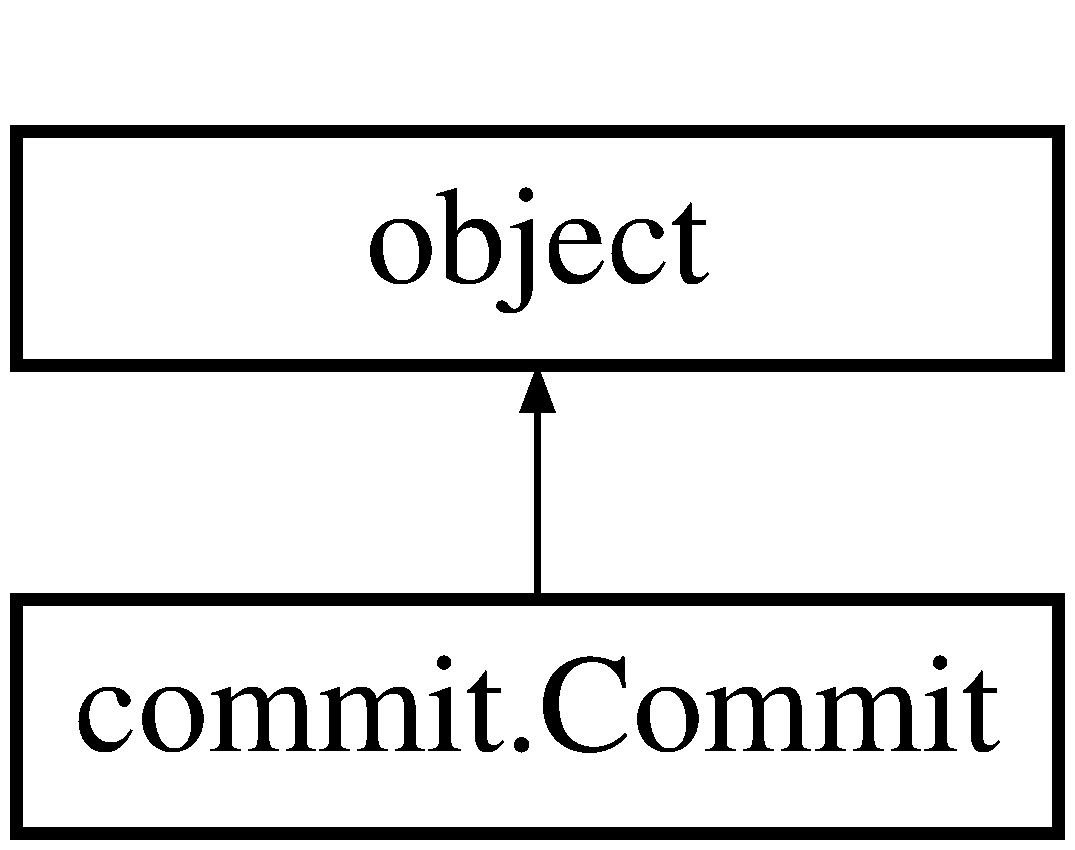
\includegraphics[height=2.000000cm]{classcommit_1_1Commit}
\end{center}
\end{figure}
\subsection*{Public Member Functions}
\begin{DoxyCompactItemize}
\item 
\mbox{\Hypertarget{classcommit_1_1Commit_afe9ef31d5f94f33365d591061b8d2352}\label{classcommit_1_1Commit_afe9ef31d5f94f33365d591061b8d2352}} 
def {\bfseries \+\_\+\+\_\+init\+\_\+\+\_\+} (self, date, commitkey, author, description, files\+Modified, files\+Added, files\+Deleted)
\end{DoxyCompactItemize}
\subsection*{Public Attributes}
\begin{DoxyCompactItemize}
\item 
\mbox{\Hypertarget{classcommit_1_1Commit_ad4bc58dc0f962ce44fee02bdfd4364a9}\label{classcommit_1_1Commit_ad4bc58dc0f962ce44fee02bdfd4364a9}} 
{\bfseries date}
\item 
\mbox{\Hypertarget{classcommit_1_1Commit_a3deeda387f99b8c8776b2993be70fa91}\label{classcommit_1_1Commit_a3deeda387f99b8c8776b2993be70fa91}} 
{\bfseries commitkey}
\item 
\mbox{\Hypertarget{classcommit_1_1Commit_af9b556e9a4eb6960290e1684e7385e3f}\label{classcommit_1_1Commit_af9b556e9a4eb6960290e1684e7385e3f}} 
{\bfseries author}
\item 
\mbox{\Hypertarget{classcommit_1_1Commit_a634ad518846e752396621450a2e023a4}\label{classcommit_1_1Commit_a634ad518846e752396621450a2e023a4}} 
{\bfseries description}
\item 
\mbox{\Hypertarget{classcommit_1_1Commit_a076c59f7dd7658e346b0f1b324e897e3}\label{classcommit_1_1Commit_a076c59f7dd7658e346b0f1b324e897e3}} 
{\bfseries files\+Modified}
\item 
\mbox{\Hypertarget{classcommit_1_1Commit_a9c1f321dc1e5eb93273e817fadee47cb}\label{classcommit_1_1Commit_a9c1f321dc1e5eb93273e817fadee47cb}} 
{\bfseries files\+Added}
\item 
\mbox{\Hypertarget{classcommit_1_1Commit_a93f616ce1afa330b887bce75e49007e4}\label{classcommit_1_1Commit_a93f616ce1afa330b887bce75e49007e4}} 
{\bfseries files\+Deleted}
\end{DoxyCompactItemize}
\subsection*{Static Public Attributes}
\begin{DoxyCompactItemize}
\item 
\mbox{\Hypertarget{classcommit_1_1Commit_ae17bc2a19f57e86ec9f97edbf5c6d92a}\label{classcommit_1_1Commit_ae17bc2a19f57e86ec9f97edbf5c6d92a}} 
string {\bfseries date} = \char`\"{}\char`\"{}
\item 
\mbox{\Hypertarget{classcommit_1_1Commit_ad8266d0f52ea558bbebabe402789c392}\label{classcommit_1_1Commit_ad8266d0f52ea558bbebabe402789c392}} 
string {\bfseries commitkey} = \char`\"{}\char`\"{}
\item 
\mbox{\Hypertarget{classcommit_1_1Commit_a81ea77c430dc4e1de39cf79bc85aea7e}\label{classcommit_1_1Commit_a81ea77c430dc4e1de39cf79bc85aea7e}} 
string {\bfseries author} = \char`\"{}\char`\"{}
\item 
\mbox{\Hypertarget{classcommit_1_1Commit_a4eaa38c5a4d1ebfa4d4432a2e6879a12}\label{classcommit_1_1Commit_a4eaa38c5a4d1ebfa4d4432a2e6879a12}} 
string {\bfseries description} = \char`\"{}\char`\"{}
\item 
\mbox{\Hypertarget{classcommit_1_1Commit_a7c444414ae1a22d4a93bbcb24f962c82}\label{classcommit_1_1Commit_a7c444414ae1a22d4a93bbcb24f962c82}} 
list {\bfseries files\+Modified} = \mbox{[}$\,$\mbox{]}
\item 
\mbox{\Hypertarget{classcommit_1_1Commit_aea356b83c751276561f5fd383d7ec7fd}\label{classcommit_1_1Commit_aea356b83c751276561f5fd383d7ec7fd}} 
list {\bfseries files\+Added} = \mbox{[}$\,$\mbox{]}
\item 
\mbox{\Hypertarget{classcommit_1_1Commit_af8bf87dd7695ca9a3a7567da542073a5}\label{classcommit_1_1Commit_af8bf87dd7695ca9a3a7567da542073a5}} 
list {\bfseries files\+Deleted} = \mbox{[}$\,$\mbox{]}
\end{DoxyCompactItemize}


The documentation for this class was generated from the following file\+:\begin{DoxyCompactItemize}
\item 
docs/commit.\+py\end{DoxyCompactItemize}

\hypertarget{classgyro_1_1drive}{}\section{gyro\+:\+:drive Class Reference}
\label{classgyro_1_1drive}\index{gyro\+::drive@{gyro\+::drive}}
\subsection*{Public Attributes}
\begin{DoxyCompactItemize}
\item 
\mbox{\Hypertarget{classgyro_1_1drive_a5b4064dc01de0802b7f6d3036885091a}\label{classgyro_1_1drive_a5b4064dc01de0802b7f6d3036885091a}} 
\hyperlink{classsensors_1_1gyro__t}{sensors\+::gyro\+\_\+t} $\ast$ {\bfseries gyro}
\item 
\mbox{\Hypertarget{classgyro_1_1drive_a76152598da7454dc162b95c1e8b6156e}\label{classgyro_1_1drive_a76152598da7454dc162b95c1e8b6156e}} 
int {\bfseries heading}
\end{DoxyCompactItemize}


The documentation for this class was generated from the following file\+:\begin{DoxyCompactItemize}
\item 
include/gyro.\+hpp\end{DoxyCompactItemize}

\hypertarget{classsensors_1_1gyro__t}{}\section{sensors\+:\+:gyro\+\_\+t Class Reference}
\label{classsensors_1_1gyro__t}\index{sensors\+::gyro\+\_\+t@{sensors\+::gyro\+\_\+t}}


{\ttfamily \#include $<$sensors.\+hpp$>$}

\subsection*{Public Member Functions}
\begin{DoxyCompactItemize}
\item 
void \hyperlink{classsensors_1_1gyro__t_a5616b7066c0eb535866f51fa55a7e22b}{reset} (void)
\item 
long \hyperlink{classsensors_1_1gyro__t_acfab48fd9d83607a599e73f054f04c0e}{value} (void)
\item 
void \hyperlink{classsensors_1_1gyro__t_a01d25ac8eb835e284da8ae7842262619}{init} (void)
\item 
\hyperlink{classsensors_1_1gyro__t_a081de8249e08672f5e289f88d1017c49}{gyro\+\_\+t} (unsigned char \+\_\+port, unsigned int \+\_\+calibration)
\end{DoxyCompactItemize}
\subsection*{Public Attributes}
\begin{DoxyCompactItemize}
\item 
\hyperlink{API_8h_a04e06985633aa933343fcfa3d7fb268d}{Gyro} \hyperlink{classsensors_1_1gyro__t_a6174c882a5151d0b1461408d40403c5e}{gyro}
\item 
unsigned char \hyperlink{classsensors_1_1gyro__t_aed9a64ee6944cef330bc769c606cb7e9}{port}
\item 
long \hyperlink{classsensors_1_1gyro__t_ac66c52c31ee9cff57a88b514a9f99051}{zero}
\item 
float \hyperlink{classsensors_1_1gyro__t_a9367db771651c0dbdf14fac3946e8582}{request}
\end{DoxyCompactItemize}


\subsection{Detailed Description}
Class for gyro objects 

\subsection{Constructor \& Destructor Documentation}
\mbox{\Hypertarget{classsensors_1_1gyro__t_a081de8249e08672f5e289f88d1017c49}\label{classsensors_1_1gyro__t_a081de8249e08672f5e289f88d1017c49}} 
\index{sensors\+::gyro\+\_\+t@{sensors\+::gyro\+\_\+t}!gyro\+\_\+t@{gyro\+\_\+t}}
\index{gyro\+\_\+t@{gyro\+\_\+t}!sensors\+::gyro\+\_\+t@{sensors\+::gyro\+\_\+t}}
\subsubsection{\texorpdfstring{gyro\+\_\+t()}{gyro\_t()}}
{\footnotesize\ttfamily sensors\+::gyro\+\_\+t\+::gyro\+\_\+t (\begin{DoxyParamCaption}\item[{unsigned char}]{\+\_\+port,  }\item[{unsigned int}]{\+\_\+calibration }\end{DoxyParamCaption})}

Class constructor, but it must not be forgotten to call \hyperlink{classsensors_1_1gyro__t_a01d25ac8eb835e284da8ae7842262619}{init()} 

\subsection{Member Function Documentation}
\mbox{\Hypertarget{classsensors_1_1gyro__t_a01d25ac8eb835e284da8ae7842262619}\label{classsensors_1_1gyro__t_a01d25ac8eb835e284da8ae7842262619}} 
\index{sensors\+::gyro\+\_\+t@{sensors\+::gyro\+\_\+t}!init@{init}}
\index{init@{init}!sensors\+::gyro\+\_\+t@{sensors\+::gyro\+\_\+t}}
\subsubsection{\texorpdfstring{init()}{init()}}
{\footnotesize\ttfamily void sensors\+::gyro\+\_\+t\+::init (\begin{DoxyParamCaption}\item[{void}]{ }\end{DoxyParamCaption})}

Initialization funtion for the gyro, call in \hyperlink{main_8h_a25a40b6614565f755233080a384c35f1}{initialize()} \mbox{\Hypertarget{classsensors_1_1gyro__t_a5616b7066c0eb535866f51fa55a7e22b}\label{classsensors_1_1gyro__t_a5616b7066c0eb535866f51fa55a7e22b}} 
\index{sensors\+::gyro\+\_\+t@{sensors\+::gyro\+\_\+t}!reset@{reset}}
\index{reset@{reset}!sensors\+::gyro\+\_\+t@{sensors\+::gyro\+\_\+t}}
\subsubsection{\texorpdfstring{reset()}{reset()}}
{\footnotesize\ttfamily void sensors\+::gyro\+\_\+t\+::reset (\begin{DoxyParamCaption}\item[{void}]{ }\end{DoxyParamCaption})}

Resets the value to 0 \mbox{\Hypertarget{classsensors_1_1gyro__t_acfab48fd9d83607a599e73f054f04c0e}\label{classsensors_1_1gyro__t_acfab48fd9d83607a599e73f054f04c0e}} 
\index{sensors\+::gyro\+\_\+t@{sensors\+::gyro\+\_\+t}!value@{value}}
\index{value@{value}!sensors\+::gyro\+\_\+t@{sensors\+::gyro\+\_\+t}}
\subsubsection{\texorpdfstring{value()}{value()}}
{\footnotesize\ttfamily long sensors\+::gyro\+\_\+t\+::value (\begin{DoxyParamCaption}\item[{void}]{ }\end{DoxyParamCaption})}

Returns the current value of the gyro, relative to the zero 

\subsection{Member Data Documentation}
\mbox{\Hypertarget{classsensors_1_1gyro__t_a6174c882a5151d0b1461408d40403c5e}\label{classsensors_1_1gyro__t_a6174c882a5151d0b1461408d40403c5e}} 
\index{sensors\+::gyro\+\_\+t@{sensors\+::gyro\+\_\+t}!gyro@{gyro}}
\index{gyro@{gyro}!sensors\+::gyro\+\_\+t@{sensors\+::gyro\+\_\+t}}
\subsubsection{\texorpdfstring{gyro}{gyro}}
{\footnotesize\ttfamily \hyperlink{API_8h_a04e06985633aa933343fcfa3d7fb268d}{Gyro} sensors\+::gyro\+\_\+t\+::gyro}

The gyro struct used in funtions \mbox{\Hypertarget{classsensors_1_1gyro__t_aed9a64ee6944cef330bc769c606cb7e9}\label{classsensors_1_1gyro__t_aed9a64ee6944cef330bc769c606cb7e9}} 
\index{sensors\+::gyro\+\_\+t@{sensors\+::gyro\+\_\+t}!port@{port}}
\index{port@{port}!sensors\+::gyro\+\_\+t@{sensors\+::gyro\+\_\+t}}
\subsubsection{\texorpdfstring{port}{port}}
{\footnotesize\ttfamily unsigned char sensors\+::gyro\+\_\+t\+::port}

The port the gyro is plugged into \mbox{\Hypertarget{classsensors_1_1gyro__t_a9367db771651c0dbdf14fac3946e8582}\label{classsensors_1_1gyro__t_a9367db771651c0dbdf14fac3946e8582}} 
\index{sensors\+::gyro\+\_\+t@{sensors\+::gyro\+\_\+t}!request@{request}}
\index{request@{request}!sensors\+::gyro\+\_\+t@{sensors\+::gyro\+\_\+t}}
\subsubsection{\texorpdfstring{request}{request}}
{\footnotesize\ttfamily float sensors\+::gyro\+\_\+t\+::request}

The pid requested value of the gyro \mbox{\Hypertarget{classsensors_1_1gyro__t_ac66c52c31ee9cff57a88b514a9f99051}\label{classsensors_1_1gyro__t_ac66c52c31ee9cff57a88b514a9f99051}} 
\index{sensors\+::gyro\+\_\+t@{sensors\+::gyro\+\_\+t}!zero@{zero}}
\index{zero@{zero}!sensors\+::gyro\+\_\+t@{sensors\+::gyro\+\_\+t}}
\subsubsection{\texorpdfstring{zero}{zero}}
{\footnotesize\ttfamily long sensors\+::gyro\+\_\+t\+::zero}

The relative zero of the gyro, such that you can add it to the returned value to obtain an absolute value 

The documentation for this class was generated from the following files\+:\begin{DoxyCompactItemize}
\item 
include/sensors.\+hpp\item 
src/sensors.\+cpp\end{DoxyCompactItemize}

\hypertarget{structmotor__t}{}\section{motor\+\_\+t Struct Reference}
\label{structmotor__t}\index{motor\+\_\+t@{motor\+\_\+t}}


{\ttfamily \#include $<$motors.\+hpp$>$}

\subsection*{Public Member Functions}
\begin{DoxyCompactItemize}
\item 
void \hyperlink{structmotor__t_abbb5dde85e4548012cf8cf796093313f}{set} (int \hyperlink{structmotor__t_a7e84d55b013193d736b66bc4d213e98f}{power})
\end{DoxyCompactItemize}
\subsection*{Public Attributes}
\begin{DoxyCompactItemize}
\item 
unsigned char \hyperlink{structmotor__t_a5b2cb1644501c09be84743b375fd2071}{port}
\item 
char \hyperlink{structmotor__t_a151da94c1625feddc6dd621d7a97f64b}{inverted}
\item 
int \hyperlink{structmotor__t_a7e84d55b013193d736b66bc4d213e98f}{power}
\item 
float \hyperlink{structmotor__t_a313fd4008216d0d01b20dcf14ee83fb6}{scale}
\item 
\mbox{\Hypertarget{structmotor__t_a226db167970cfe00376b7fbaca6e8d13}\label{structmotor__t_a226db167970cfe00376b7fbaca6e8d13}} 
float {\bfseries slew\+Rate}
\item 
unsigned long \hyperlink{structmotor__t_a4f00b961c42d53610d71bb90efdcd089}{tlast}
\end{DoxyCompactItemize}


\subsection{Detailed Description}
Class for motor objects 

\subsection{Member Function Documentation}
\mbox{\Hypertarget{structmotor__t_abbb5dde85e4548012cf8cf796093313f}\label{structmotor__t_abbb5dde85e4548012cf8cf796093313f}} 
\index{motor\+\_\+t@{motor\+\_\+t}!set@{set}}
\index{set@{set}!motor\+\_\+t@{motor\+\_\+t}}
\subsubsection{\texorpdfstring{set()}{set()}}
{\footnotesize\ttfamily void motor\+\_\+t\+::set (\begin{DoxyParamCaption}\item[{int}]{power }\end{DoxyParamCaption})}

Set the motor to the specified power 

\subsection{Member Data Documentation}
\mbox{\Hypertarget{structmotor__t_a151da94c1625feddc6dd621d7a97f64b}\label{structmotor__t_a151da94c1625feddc6dd621d7a97f64b}} 
\index{motor\+\_\+t@{motor\+\_\+t}!inverted@{inverted}}
\index{inverted@{inverted}!motor\+\_\+t@{motor\+\_\+t}}
\subsubsection{\texorpdfstring{inverted}{inverted}}
{\footnotesize\ttfamily char motor\+\_\+t\+::inverted}

The invered status of the motor, should be 1 or -\/1 \mbox{\Hypertarget{structmotor__t_a5b2cb1644501c09be84743b375fd2071}\label{structmotor__t_a5b2cb1644501c09be84743b375fd2071}} 
\index{motor\+\_\+t@{motor\+\_\+t}!port@{port}}
\index{port@{port}!motor\+\_\+t@{motor\+\_\+t}}
\subsubsection{\texorpdfstring{port}{port}}
{\footnotesize\ttfamily unsigned char motor\+\_\+t\+::port}

Port the motor is pluggin in to \mbox{\Hypertarget{structmotor__t_a7e84d55b013193d736b66bc4d213e98f}\label{structmotor__t_a7e84d55b013193d736b66bc4d213e98f}} 
\index{motor\+\_\+t@{motor\+\_\+t}!power@{power}}
\index{power@{power}!motor\+\_\+t@{motor\+\_\+t}}
\subsubsection{\texorpdfstring{power}{power}}
{\footnotesize\ttfamily int motor\+\_\+t\+::power}

The requested power value of the motor \mbox{\Hypertarget{structmotor__t_a313fd4008216d0d01b20dcf14ee83fb6}\label{structmotor__t_a313fd4008216d0d01b20dcf14ee83fb6}} 
\index{motor\+\_\+t@{motor\+\_\+t}!scale@{scale}}
\index{scale@{scale}!motor\+\_\+t@{motor\+\_\+t}}
\subsubsection{\texorpdfstring{scale}{scale}}
{\footnotesize\ttfamily float motor\+\_\+t\+::scale}

A multiplier for setting the motor values \mbox{\Hypertarget{structmotor__t_a4f00b961c42d53610d71bb90efdcd089}\label{structmotor__t_a4f00b961c42d53610d71bb90efdcd089}} 
\index{motor\+\_\+t@{motor\+\_\+t}!tlast@{tlast}}
\index{tlast@{tlast}!motor\+\_\+t@{motor\+\_\+t}}
\subsubsection{\texorpdfstring{tlast}{tlast}}
{\footnotesize\ttfamily unsigned long motor\+\_\+t\+::tlast}

The last update time of the motor. Is managed by the slew task, so it shouldn\textquotesingle{}t need to be changed 

The documentation for this struct was generated from the following files\+:\begin{DoxyCompactItemize}
\item 
include/motors.\+hpp\item 
src/motors.\+cpp\end{DoxyCompactItemize}

\hypertarget{structsensors_1_1pot__t}{}\section{sensors\+:\+:pot\+\_\+t Struct Reference}
\label{structsensors_1_1pot__t}\index{sensors\+::pot\+\_\+t@{sensors\+::pot\+\_\+t}}


{\ttfamily \#include $<$sensors.\+hpp$>$}

\subsection*{Public Member Functions}
\begin{DoxyCompactItemize}
\item 
void \hyperlink{structsensors_1_1pot__t_a79492a67771f5cf54b4efcc6ca0178b5}{reset} (void)
\item 
long \hyperlink{structsensors_1_1pot__t_a239236592ff0507f459f6e8d40d12816}{value} (void)
\item 
void \hyperlink{structsensors_1_1pot__t_ab44d6b91085fd38241c4c83b8f1cade1}{init} (void)
\item 
\hyperlink{structsensors_1_1pot__t_a118a5459f2e27e5823651172c43c30f8}{pot\+\_\+t} (unsigned char \+\_\+port, bool \+\_\+inverted)
\end{DoxyCompactItemize}
\subsection*{Public Attributes}
\begin{DoxyCompactItemize}
\item 
unsigned char \hyperlink{structsensors_1_1pot__t_a1bf5ff29049431caa618b0016421b7f2}{port}
\item 
long \hyperlink{structsensors_1_1pot__t_ad3678a63f0a9f4d3d3e864ec22161764}{zero}
\item 
bool \hyperlink{structsensors_1_1pot__t_a123c1d2c33ce2fe9284ade146451b987}{inverted}
\item 
float \hyperlink{structsensors_1_1pot__t_a364b3294c1c4a7b5247663b48189f8a5}{request}
\end{DoxyCompactItemize}


\subsection{Detailed Description}
Class for potentiometers 

\subsection{Constructor \& Destructor Documentation}
\mbox{\Hypertarget{structsensors_1_1pot__t_a118a5459f2e27e5823651172c43c30f8}\label{structsensors_1_1pot__t_a118a5459f2e27e5823651172c43c30f8}} 
\index{sensors\+::pot\+\_\+t@{sensors\+::pot\+\_\+t}!pot\+\_\+t@{pot\+\_\+t}}
\index{pot\+\_\+t@{pot\+\_\+t}!sensors\+::pot\+\_\+t@{sensors\+::pot\+\_\+t}}
\subsubsection{\texorpdfstring{pot\+\_\+t()}{pot\_t()}}
{\footnotesize\ttfamily sensors\+::pot\+\_\+t\+::pot\+\_\+t (\begin{DoxyParamCaption}\item[{unsigned char}]{\+\_\+port,  }\item[{bool}]{\+\_\+inverted }\end{DoxyParamCaption})}

The class constructor for a potentiometer, also be sure to \hyperlink{structsensors_1_1pot__t_ab44d6b91085fd38241c4c83b8f1cade1}{init()} 

\subsection{Member Function Documentation}
\mbox{\Hypertarget{structsensors_1_1pot__t_ab44d6b91085fd38241c4c83b8f1cade1}\label{structsensors_1_1pot__t_ab44d6b91085fd38241c4c83b8f1cade1}} 
\index{sensors\+::pot\+\_\+t@{sensors\+::pot\+\_\+t}!init@{init}}
\index{init@{init}!sensors\+::pot\+\_\+t@{sensors\+::pot\+\_\+t}}
\subsubsection{\texorpdfstring{init()}{init()}}
{\footnotesize\ttfamily void sensors\+::pot\+\_\+t\+::init (\begin{DoxyParamCaption}\item[{void}]{ }\end{DoxyParamCaption})}

The initialization funtion for the potentiometer, which must be called in \hyperlink{main_8h_a25a40b6614565f755233080a384c35f1}{initialize()} \mbox{\Hypertarget{structsensors_1_1pot__t_a79492a67771f5cf54b4efcc6ca0178b5}\label{structsensors_1_1pot__t_a79492a67771f5cf54b4efcc6ca0178b5}} 
\index{sensors\+::pot\+\_\+t@{sensors\+::pot\+\_\+t}!reset@{reset}}
\index{reset@{reset}!sensors\+::pot\+\_\+t@{sensors\+::pot\+\_\+t}}
\subsubsection{\texorpdfstring{reset()}{reset()}}
{\footnotesize\ttfamily void sensors\+::pot\+\_\+t\+::reset (\begin{DoxyParamCaption}\item[{void}]{ }\end{DoxyParamCaption})}

Resets the value to 0 \mbox{\Hypertarget{structsensors_1_1pot__t_a239236592ff0507f459f6e8d40d12816}\label{structsensors_1_1pot__t_a239236592ff0507f459f6e8d40d12816}} 
\index{sensors\+::pot\+\_\+t@{sensors\+::pot\+\_\+t}!value@{value}}
\index{value@{value}!sensors\+::pot\+\_\+t@{sensors\+::pot\+\_\+t}}
\subsubsection{\texorpdfstring{value()}{value()}}
{\footnotesize\ttfamily long sensors\+::pot\+\_\+t\+::value (\begin{DoxyParamCaption}\item[{void}]{ }\end{DoxyParamCaption})}

Returns the relative value of the potentiometer 

\subsection{Member Data Documentation}
\mbox{\Hypertarget{structsensors_1_1pot__t_a123c1d2c33ce2fe9284ade146451b987}\label{structsensors_1_1pot__t_a123c1d2c33ce2fe9284ade146451b987}} 
\index{sensors\+::pot\+\_\+t@{sensors\+::pot\+\_\+t}!inverted@{inverted}}
\index{inverted@{inverted}!sensors\+::pot\+\_\+t@{sensors\+::pot\+\_\+t}}
\subsubsection{\texorpdfstring{inverted}{inverted}}
{\footnotesize\ttfamily bool sensors\+::pot\+\_\+t\+::inverted}

Whether or not the potentioeter\textquotesingle{}s value should be inverted \mbox{\Hypertarget{structsensors_1_1pot__t_a1bf5ff29049431caa618b0016421b7f2}\label{structsensors_1_1pot__t_a1bf5ff29049431caa618b0016421b7f2}} 
\index{sensors\+::pot\+\_\+t@{sensors\+::pot\+\_\+t}!port@{port}}
\index{port@{port}!sensors\+::pot\+\_\+t@{sensors\+::pot\+\_\+t}}
\subsubsection{\texorpdfstring{port}{port}}
{\footnotesize\ttfamily unsigned char sensors\+::pot\+\_\+t\+::port}

The port that the pot is plugged in to \mbox{\Hypertarget{structsensors_1_1pot__t_a364b3294c1c4a7b5247663b48189f8a5}\label{structsensors_1_1pot__t_a364b3294c1c4a7b5247663b48189f8a5}} 
\index{sensors\+::pot\+\_\+t@{sensors\+::pot\+\_\+t}!request@{request}}
\index{request@{request}!sensors\+::pot\+\_\+t@{sensors\+::pot\+\_\+t}}
\subsubsection{\texorpdfstring{request}{request}}
{\footnotesize\ttfamily float sensors\+::pot\+\_\+t\+::request}

The pid requested value of the pot \mbox{\Hypertarget{structsensors_1_1pot__t_ad3678a63f0a9f4d3d3e864ec22161764}\label{structsensors_1_1pot__t_ad3678a63f0a9f4d3d3e864ec22161764}} 
\index{sensors\+::pot\+\_\+t@{sensors\+::pot\+\_\+t}!zero@{zero}}
\index{zero@{zero}!sensors\+::pot\+\_\+t@{sensors\+::pot\+\_\+t}}
\subsubsection{\texorpdfstring{zero}{zero}}
{\footnotesize\ttfamily long sensors\+::pot\+\_\+t\+::zero}

The relative zero, that can be added to the returned \hyperlink{structsensors_1_1pot__t_a239236592ff0507f459f6e8d40d12816}{value()} to find the absolute value 

The documentation for this struct was generated from the following files\+:\begin{DoxyCompactItemize}
\item 
include/sensors.\+hpp\item 
src/sensors.\+cpp\end{DoxyCompactItemize}

\hypertarget{structsensors_1_1quad__t}{}\section{sensors\+:\+:quad\+\_\+t Struct Reference}
\label{structsensors_1_1quad__t}\index{sensors\+::quad\+\_\+t@{sensors\+::quad\+\_\+t}}


{\ttfamily \#include $<$sensors.\+hpp$>$}

\subsection*{Public Member Functions}
\begin{DoxyCompactItemize}
\item 
void \hyperlink{structsensors_1_1quad__t_ab68ad73b35c435a8b3419403c0e95b74}{reset} (void)
\item 
long \hyperlink{structsensors_1_1quad__t_a5d05cb2d530870f1108c4181715f7006}{value} (void)
\item 
void \hyperlink{structsensors_1_1quad__t_a27e6a2d1744cea7570b81fb03086cfa4}{init} (void)
\item 
\hyperlink{structsensors_1_1quad__t_a5d32ea19d30a4b33e6d99f94df08b9e7}{quad\+\_\+t} (unsigned char port1, unsigned char port2, bool \+\_\+inverted)
\end{DoxyCompactItemize}
\subsection*{Public Attributes}
\begin{DoxyCompactItemize}
\item 
\hyperlink{API_8h_a8289b20280bf9db1462f60dae76d2939}{Encoder} \hyperlink{structsensors_1_1quad__t_ab6355ae9a56dea947376ccfd2b3b9da8}{enc}
\item 
unsigned char \hyperlink{structsensors_1_1quad__t_ab3ac2cbedde9a5d8cb680e8c4bcdec74}{ports} \mbox{[}2\mbox{]}
\item 
long \hyperlink{structsensors_1_1quad__t_a06d5116929f4ed2878d452c02470c644}{zero}
\item 
bool \hyperlink{structsensors_1_1quad__t_a7c95cf6e860fa651b3dc23535d5e1407}{inverted}
\item 
float \hyperlink{structsensors_1_1quad__t_ab1cf656f73ea0165459e90c035c0b03c}{request}
\end{DoxyCompactItemize}


\subsection{Detailed Description}
A 2-\/wire quadrature encoder 

\subsection{Constructor \& Destructor Documentation}
\mbox{\Hypertarget{structsensors_1_1quad__t_a5d32ea19d30a4b33e6d99f94df08b9e7}\label{structsensors_1_1quad__t_a5d32ea19d30a4b33e6d99f94df08b9e7}} 
\index{sensors\+::quad\+\_\+t@{sensors\+::quad\+\_\+t}!quad\+\_\+t@{quad\+\_\+t}}
\index{quad\+\_\+t@{quad\+\_\+t}!sensors\+::quad\+\_\+t@{sensors\+::quad\+\_\+t}}
\subsubsection{\texorpdfstring{quad\+\_\+t()}{quad\_t()}}
{\footnotesize\ttfamily sensors\+::quad\+\_\+t\+::quad\+\_\+t (\begin{DoxyParamCaption}\item[{unsigned char}]{port1,  }\item[{unsigned char}]{port2,  }\item[{bool}]{\+\_\+inverted }\end{DoxyParamCaption})}

Constructs the encoder object. Make sure init is also called 

\subsection{Member Function Documentation}
\mbox{\Hypertarget{structsensors_1_1quad__t_a27e6a2d1744cea7570b81fb03086cfa4}\label{structsensors_1_1quad__t_a27e6a2d1744cea7570b81fb03086cfa4}} 
\index{sensors\+::quad\+\_\+t@{sensors\+::quad\+\_\+t}!init@{init}}
\index{init@{init}!sensors\+::quad\+\_\+t@{sensors\+::quad\+\_\+t}}
\subsubsection{\texorpdfstring{init()}{init()}}
{\footnotesize\ttfamily void sensors\+::quad\+\_\+t\+::init (\begin{DoxyParamCaption}\item[{void}]{ }\end{DoxyParamCaption})}

The initialization function for the encoder. Call in \hyperlink{main_8h_a25a40b6614565f755233080a384c35f1}{initialize()} \mbox{\Hypertarget{structsensors_1_1quad__t_ab68ad73b35c435a8b3419403c0e95b74}\label{structsensors_1_1quad__t_ab68ad73b35c435a8b3419403c0e95b74}} 
\index{sensors\+::quad\+\_\+t@{sensors\+::quad\+\_\+t}!reset@{reset}}
\index{reset@{reset}!sensors\+::quad\+\_\+t@{sensors\+::quad\+\_\+t}}
\subsubsection{\texorpdfstring{reset()}{reset()}}
{\footnotesize\ttfamily void sensors\+::quad\+\_\+t\+::reset (\begin{DoxyParamCaption}\item[{void}]{ }\end{DoxyParamCaption})}

Reset the value to zero \mbox{\Hypertarget{structsensors_1_1quad__t_a5d05cb2d530870f1108c4181715f7006}\label{structsensors_1_1quad__t_a5d05cb2d530870f1108c4181715f7006}} 
\index{sensors\+::quad\+\_\+t@{sensors\+::quad\+\_\+t}!value@{value}}
\index{value@{value}!sensors\+::quad\+\_\+t@{sensors\+::quad\+\_\+t}}
\subsubsection{\texorpdfstring{value()}{value()}}
{\footnotesize\ttfamily long sensors\+::quad\+\_\+t\+::value (\begin{DoxyParamCaption}\item[{void}]{ }\end{DoxyParamCaption})}

Returns the relative value of the encoder. If added to the encoder\textquotesingle{}s zero, produces an absolute value of the encoder 

\subsection{Member Data Documentation}
\mbox{\Hypertarget{structsensors_1_1quad__t_ab6355ae9a56dea947376ccfd2b3b9da8}\label{structsensors_1_1quad__t_ab6355ae9a56dea947376ccfd2b3b9da8}} 
\index{sensors\+::quad\+\_\+t@{sensors\+::quad\+\_\+t}!enc@{enc}}
\index{enc@{enc}!sensors\+::quad\+\_\+t@{sensors\+::quad\+\_\+t}}
\subsubsection{\texorpdfstring{enc}{enc}}
{\footnotesize\ttfamily \hyperlink{API_8h_a8289b20280bf9db1462f60dae76d2939}{Encoder} sensors\+::quad\+\_\+t\+::enc}

The encoder struct used by other member functions \mbox{\Hypertarget{structsensors_1_1quad__t_a7c95cf6e860fa651b3dc23535d5e1407}\label{structsensors_1_1quad__t_a7c95cf6e860fa651b3dc23535d5e1407}} 
\index{sensors\+::quad\+\_\+t@{sensors\+::quad\+\_\+t}!inverted@{inverted}}
\index{inverted@{inverted}!sensors\+::quad\+\_\+t@{sensors\+::quad\+\_\+t}}
\subsubsection{\texorpdfstring{inverted}{inverted}}
{\footnotesize\ttfamily bool sensors\+::quad\+\_\+t\+::inverted}

Whether or not the encoder is inverted \mbox{\Hypertarget{structsensors_1_1quad__t_ab3ac2cbedde9a5d8cb680e8c4bcdec74}\label{structsensors_1_1quad__t_ab3ac2cbedde9a5d8cb680e8c4bcdec74}} 
\index{sensors\+::quad\+\_\+t@{sensors\+::quad\+\_\+t}!ports@{ports}}
\index{ports@{ports}!sensors\+::quad\+\_\+t@{sensors\+::quad\+\_\+t}}
\subsubsection{\texorpdfstring{ports}{ports}}
{\footnotesize\ttfamily unsigned char sensors\+::quad\+\_\+t\+::ports\mbox{[}2\mbox{]}}

The ports the encoder is connected to, in order of top, then bottom, when the removable cover is facing up \mbox{\Hypertarget{structsensors_1_1quad__t_ab1cf656f73ea0165459e90c035c0b03c}\label{structsensors_1_1quad__t_ab1cf656f73ea0165459e90c035c0b03c}} 
\index{sensors\+::quad\+\_\+t@{sensors\+::quad\+\_\+t}!request@{request}}
\index{request@{request}!sensors\+::quad\+\_\+t@{sensors\+::quad\+\_\+t}}
\subsubsection{\texorpdfstring{request}{request}}
{\footnotesize\ttfamily float sensors\+::quad\+\_\+t\+::request}

The pid requested value of the encoder \mbox{\Hypertarget{structsensors_1_1quad__t_a06d5116929f4ed2878d452c02470c644}\label{structsensors_1_1quad__t_a06d5116929f4ed2878d452c02470c644}} 
\index{sensors\+::quad\+\_\+t@{sensors\+::quad\+\_\+t}!zero@{zero}}
\index{zero@{zero}!sensors\+::quad\+\_\+t@{sensors\+::quad\+\_\+t}}
\subsubsection{\texorpdfstring{zero}{zero}}
{\footnotesize\ttfamily long sensors\+::quad\+\_\+t\+::zero}

The relative zero from which the encoder\textquotesingle{}s value will be returned. Can be added to returned value to produce a true value for the encoder 

The documentation for this struct was generated from the following files\+:\begin{DoxyCompactItemize}
\item 
/home/ethan/\+V\+E\+X-\/709\+S-\/2018/include/sensors.\+hpp\item 
/home/ethan/\+V\+E\+X-\/709\+S-\/2018/src/sensors.\+cpp\end{DoxyCompactItemize}

\hypertarget{structdrive_1_1side__t}{}\section{drive\+:\+:side\+\_\+t Struct Reference}
\label{structdrive_1_1side__t}\index{drive\+::side\+\_\+t@{drive\+::side\+\_\+t}}


{\ttfamily \#include $<$drive.\+hpp$>$}

\subsection*{Public Member Functions}
\begin{DoxyCompactItemize}
\item 
void \hyperlink{structdrive_1_1side__t_ab605b00c5f98faa239cab1b19b54e7e6}{set} (int power)
\end{DoxyCompactItemize}
\subsection*{Public Attributes}
\begin{DoxyCompactItemize}
\item 
\hyperlink{structmotor__t}{motor\+\_\+t} \hyperlink{structdrive_1_1side__t_a3a32e841a8f53200b37c040572765165}{topM}
\item 
\hyperlink{structmotor__t}{motor\+\_\+t} \hyperlink{structdrive_1_1side__t_acb33aa4a812f555b5fa0e94882d6e91a}{midM}
\item 
\hyperlink{structmotor__t}{motor\+\_\+t} \hyperlink{structdrive_1_1side__t_a38de3f1053b41c5b2824ffed7ab8c32a}{lowM}
\item 
\hyperlink{structsensors_1_1quad__t}{sensors\+::quad\+\_\+t} $\ast$ \hyperlink{structdrive_1_1side__t_a50f80a71f0be44bbb8df9b7f3f81aedf}{sensor}
\end{DoxyCompactItemize}


\subsection{Detailed Description}
Class for a side of the drive 

\subsection{Member Function Documentation}
\mbox{\Hypertarget{structdrive_1_1side__t_ab605b00c5f98faa239cab1b19b54e7e6}\label{structdrive_1_1side__t_ab605b00c5f98faa239cab1b19b54e7e6}} 
\index{drive\+::side\+\_\+t@{drive\+::side\+\_\+t}!set@{set}}
\index{set@{set}!drive\+::side\+\_\+t@{drive\+::side\+\_\+t}}
\subsubsection{\texorpdfstring{set()}{set()}}
{\footnotesize\ttfamily void drive\+::side\+\_\+t\+::set (\begin{DoxyParamCaption}\item[{int}]{power }\end{DoxyParamCaption})}

Sets all motors on the side to the given power 

\subsection{Member Data Documentation}
\mbox{\Hypertarget{structdrive_1_1side__t_a38de3f1053b41c5b2824ffed7ab8c32a}\label{structdrive_1_1side__t_a38de3f1053b41c5b2824ffed7ab8c32a}} 
\index{drive\+::side\+\_\+t@{drive\+::side\+\_\+t}!lowM@{lowM}}
\index{lowM@{lowM}!drive\+::side\+\_\+t@{drive\+::side\+\_\+t}}
\subsubsection{\texorpdfstring{lowM}{lowM}}
{\footnotesize\ttfamily \hyperlink{structmotor__t}{motor\+\_\+t} drive\+::side\+\_\+t\+::lowM}

Bottom motor on the side \mbox{\Hypertarget{structdrive_1_1side__t_acb33aa4a812f555b5fa0e94882d6e91a}\label{structdrive_1_1side__t_acb33aa4a812f555b5fa0e94882d6e91a}} 
\index{drive\+::side\+\_\+t@{drive\+::side\+\_\+t}!midM@{midM}}
\index{midM@{midM}!drive\+::side\+\_\+t@{drive\+::side\+\_\+t}}
\subsubsection{\texorpdfstring{midM}{midM}}
{\footnotesize\ttfamily \hyperlink{structmotor__t}{motor\+\_\+t} drive\+::side\+\_\+t\+::midM}

Middle motor on the side \mbox{\Hypertarget{structdrive_1_1side__t_a50f80a71f0be44bbb8df9b7f3f81aedf}\label{structdrive_1_1side__t_a50f80a71f0be44bbb8df9b7f3f81aedf}} 
\index{drive\+::side\+\_\+t@{drive\+::side\+\_\+t}!sensor@{sensor}}
\index{sensor@{sensor}!drive\+::side\+\_\+t@{drive\+::side\+\_\+t}}
\subsubsection{\texorpdfstring{sensor}{sensor}}
{\footnotesize\ttfamily \hyperlink{structsensors_1_1quad__t}{sensors\+::quad\+\_\+t}$\ast$ drive\+::side\+\_\+t\+::sensor}

A pointer to the sensor on the side \mbox{\Hypertarget{structdrive_1_1side__t_a3a32e841a8f53200b37c040572765165}\label{structdrive_1_1side__t_a3a32e841a8f53200b37c040572765165}} 
\index{drive\+::side\+\_\+t@{drive\+::side\+\_\+t}!topM@{topM}}
\index{topM@{topM}!drive\+::side\+\_\+t@{drive\+::side\+\_\+t}}
\subsubsection{\texorpdfstring{topM}{topM}}
{\footnotesize\ttfamily \hyperlink{structmotor__t}{motor\+\_\+t} drive\+::side\+\_\+t\+::topM}

Top motor on the the side 

The documentation for this struct was generated from the following files\+:\begin{DoxyCompactItemize}
\item 
include/drive.\+hpp\item 
src/drive.\+cpp\end{DoxyCompactItemize}

\hypertarget{structlift_1_1side__t}{}\section{lift\+:\+:side\+\_\+t Struct Reference}
\label{structlift_1_1side__t}\index{lift\+::side\+\_\+t@{lift\+::side\+\_\+t}}


{\ttfamily \#include $<$lift.\+hpp$>$}

\subsection*{Public Member Functions}
\begin{DoxyCompactItemize}
\item 
void \hyperlink{structlift_1_1side__t_af7e51af6ba1f15f1a522139e8c18f047}{set} (int power)
\end{DoxyCompactItemize}
\subsection*{Public Attributes}
\begin{DoxyCompactItemize}
\item 
\hyperlink{structmotor__t}{motor\+\_\+t} \hyperlink{structlift_1_1side__t_a98eccfefb378ed0a246a5f74a95f9020}{topM}
\item 
\hyperlink{structmotor__t}{motor\+\_\+t} \hyperlink{structlift_1_1side__t_a83c244448926521665e0f4d664b7b2b3}{midM}
\item 
\hyperlink{structmotor__t}{motor\+\_\+t} \hyperlink{structlift_1_1side__t_a9c945e15eea72e044cd3c5303b775059}{lowM}
\item 
\hyperlink{structsensors_1_1pot__t}{sensors\+::pot\+\_\+t} $\ast$ \hyperlink{structlift_1_1side__t_a8216f7c176f2fc4f17bc8f6ce6d53fcd}{sensor}
\end{DoxyCompactItemize}


\subsection{Detailed Description}
Class for a side of the drive 

\subsection{Member Function Documentation}
\mbox{\Hypertarget{structlift_1_1side__t_af7e51af6ba1f15f1a522139e8c18f047}\label{structlift_1_1side__t_af7e51af6ba1f15f1a522139e8c18f047}} 
\index{lift\+::side\+\_\+t@{lift\+::side\+\_\+t}!set@{set}}
\index{set@{set}!lift\+::side\+\_\+t@{lift\+::side\+\_\+t}}
\subsubsection{\texorpdfstring{set()}{set()}}
{\footnotesize\ttfamily void lift\+::side\+\_\+t\+::set (\begin{DoxyParamCaption}\item[{int}]{power }\end{DoxyParamCaption})}

Sets all motors on the side to the given power 

\subsection{Member Data Documentation}
\mbox{\Hypertarget{structlift_1_1side__t_a9c945e15eea72e044cd3c5303b775059}\label{structlift_1_1side__t_a9c945e15eea72e044cd3c5303b775059}} 
\index{lift\+::side\+\_\+t@{lift\+::side\+\_\+t}!lowM@{lowM}}
\index{lowM@{lowM}!lift\+::side\+\_\+t@{lift\+::side\+\_\+t}}
\subsubsection{\texorpdfstring{lowM}{lowM}}
{\footnotesize\ttfamily \hyperlink{structmotor__t}{motor\+\_\+t} lift\+::side\+\_\+t\+::lowM}

Bottom motor on the side \mbox{\Hypertarget{structlift_1_1side__t_a83c244448926521665e0f4d664b7b2b3}\label{structlift_1_1side__t_a83c244448926521665e0f4d664b7b2b3}} 
\index{lift\+::side\+\_\+t@{lift\+::side\+\_\+t}!midM@{midM}}
\index{midM@{midM}!lift\+::side\+\_\+t@{lift\+::side\+\_\+t}}
\subsubsection{\texorpdfstring{midM}{midM}}
{\footnotesize\ttfamily \hyperlink{structmotor__t}{motor\+\_\+t} lift\+::side\+\_\+t\+::midM}

Middle motor on the side \mbox{\Hypertarget{structlift_1_1side__t_a8216f7c176f2fc4f17bc8f6ce6d53fcd}\label{structlift_1_1side__t_a8216f7c176f2fc4f17bc8f6ce6d53fcd}} 
\index{lift\+::side\+\_\+t@{lift\+::side\+\_\+t}!sensor@{sensor}}
\index{sensor@{sensor}!lift\+::side\+\_\+t@{lift\+::side\+\_\+t}}
\subsubsection{\texorpdfstring{sensor}{sensor}}
{\footnotesize\ttfamily \hyperlink{structsensors_1_1pot__t}{sensors\+::pot\+\_\+t}$\ast$ lift\+::side\+\_\+t\+::sensor}

A pointer to the sensor on the side \mbox{\Hypertarget{structlift_1_1side__t_a98eccfefb378ed0a246a5f74a95f9020}\label{structlift_1_1side__t_a98eccfefb378ed0a246a5f74a95f9020}} 
\index{lift\+::side\+\_\+t@{lift\+::side\+\_\+t}!topM@{topM}}
\index{topM@{topM}!lift\+::side\+\_\+t@{lift\+::side\+\_\+t}}
\subsubsection{\texorpdfstring{topM}{topM}}
{\footnotesize\ttfamily \hyperlink{structmotor__t}{motor\+\_\+t} lift\+::side\+\_\+t\+::topM}

Top motor on the the side 

The documentation for this struct was generated from the following files\+:\begin{DoxyCompactItemize}
\item 
/home/ethan/\+V\+E\+X-\/709\+S-\/2018/include/lift.\+hpp\item 
/home/ethan/\+V\+E\+X-\/709\+S-\/2018/src/lift.\+cpp\end{DoxyCompactItemize}

\hypertarget{structsensors_1_1sonic__t}{}\section{sensors\+:\+:sonic\+\_\+t Struct Reference}
\label{structsensors_1_1sonic__t}\index{sensors\+::sonic\+\_\+t@{sensors\+::sonic\+\_\+t}}


{\ttfamily \#include $<$sensors.\+hpp$>$}

\subsection*{Public Member Functions}
\begin{DoxyCompactItemize}
\item 
long \hyperlink{structsensors_1_1sonic__t_ac7f36354ed56c69a46efcccf9775c3d5}{value} (void)
\item 
void \hyperlink{structsensors_1_1sonic__t_a73cb49a56e55db64b42b5a6b604419dd}{init} (void)
\item 
\hyperlink{structsensors_1_1sonic__t_a29685163eb3f2fd6335fbadbcf98901e}{sonic\+\_\+t} (unsigned char port1, unsigned char port2)
\end{DoxyCompactItemize}
\subsection*{Public Attributes}
\begin{DoxyCompactItemize}
\item 
\hyperlink{API_8h_a527ee5b64142c3505d6931d8ed7ac6b7}{Ultrasonic} \hyperlink{structsensors_1_1sonic__t_ac84ca5638a8dc7156d90937eb228ed18}{sonic}
\item 
unsigned char \hyperlink{structsensors_1_1sonic__t_a64b68ab2ff696f95714dad492ea30939}{ports} \mbox{[}2\mbox{]}
\end{DoxyCompactItemize}


\subsection{Detailed Description}
Class for ultrasonic sensors 

\subsection{Constructor \& Destructor Documentation}
\mbox{\Hypertarget{structsensors_1_1sonic__t_a29685163eb3f2fd6335fbadbcf98901e}\label{structsensors_1_1sonic__t_a29685163eb3f2fd6335fbadbcf98901e}} 
\index{sensors\+::sonic\+\_\+t@{sensors\+::sonic\+\_\+t}!sonic\+\_\+t@{sonic\+\_\+t}}
\index{sonic\+\_\+t@{sonic\+\_\+t}!sensors\+::sonic\+\_\+t@{sensors\+::sonic\+\_\+t}}
\subsubsection{\texorpdfstring{sonic\+\_\+t()}{sonic\_t()}}
{\footnotesize\ttfamily sensors\+::sonic\+\_\+t\+::sonic\+\_\+t (\begin{DoxyParamCaption}\item[{unsigned char}]{port1,  }\item[{unsigned char}]{port2 }\end{DoxyParamCaption})}

Class constructor, but \hyperlink{structsensors_1_1sonic__t_a73cb49a56e55db64b42b5a6b604419dd}{init()} must also be called 

\subsection{Member Function Documentation}
\mbox{\Hypertarget{structsensors_1_1sonic__t_a73cb49a56e55db64b42b5a6b604419dd}\label{structsensors_1_1sonic__t_a73cb49a56e55db64b42b5a6b604419dd}} 
\index{sensors\+::sonic\+\_\+t@{sensors\+::sonic\+\_\+t}!init@{init}}
\index{init@{init}!sensors\+::sonic\+\_\+t@{sensors\+::sonic\+\_\+t}}
\subsubsection{\texorpdfstring{init()}{init()}}
{\footnotesize\ttfamily void sensors\+::sonic\+\_\+t\+::init (\begin{DoxyParamCaption}\item[{void}]{ }\end{DoxyParamCaption})}

Initializes the sensor. Call in \hyperlink{main_8h_a25a40b6614565f755233080a384c35f1}{initialize()} \mbox{\Hypertarget{structsensors_1_1sonic__t_ac7f36354ed56c69a46efcccf9775c3d5}\label{structsensors_1_1sonic__t_ac7f36354ed56c69a46efcccf9775c3d5}} 
\index{sensors\+::sonic\+\_\+t@{sensors\+::sonic\+\_\+t}!value@{value}}
\index{value@{value}!sensors\+::sonic\+\_\+t@{sensors\+::sonic\+\_\+t}}
\subsubsection{\texorpdfstring{value()}{value()}}
{\footnotesize\ttfamily long sensors\+::sonic\+\_\+t\+::value (\begin{DoxyParamCaption}\item[{void}]{ }\end{DoxyParamCaption})}

The value of the ultrasonic sensor 

\subsection{Member Data Documentation}
\mbox{\Hypertarget{structsensors_1_1sonic__t_a64b68ab2ff696f95714dad492ea30939}\label{structsensors_1_1sonic__t_a64b68ab2ff696f95714dad492ea30939}} 
\index{sensors\+::sonic\+\_\+t@{sensors\+::sonic\+\_\+t}!ports@{ports}}
\index{ports@{ports}!sensors\+::sonic\+\_\+t@{sensors\+::sonic\+\_\+t}}
\subsubsection{\texorpdfstring{ports}{ports}}
{\footnotesize\ttfamily unsigned char sensors\+::sonic\+\_\+t\+::ports\mbox{[}2\mbox{]}}

The two ports the sensor is plugged in to, in order of the echo (aka orange) cable, then the ping (aka yellow) cable \mbox{\Hypertarget{structsensors_1_1sonic__t_ac84ca5638a8dc7156d90937eb228ed18}\label{structsensors_1_1sonic__t_ac84ca5638a8dc7156d90937eb228ed18}} 
\index{sensors\+::sonic\+\_\+t@{sensors\+::sonic\+\_\+t}!sonic@{sonic}}
\index{sonic@{sonic}!sensors\+::sonic\+\_\+t@{sensors\+::sonic\+\_\+t}}
\subsubsection{\texorpdfstring{sonic}{sonic}}
{\footnotesize\ttfamily \hyperlink{API_8h_a527ee5b64142c3505d6931d8ed7ac6b7}{Ultrasonic} sensors\+::sonic\+\_\+t\+::sonic}

The Ultrasonic struct that is referenced in member funtions 

The documentation for this struct was generated from the following files\+:\begin{DoxyCompactItemize}
\item 
include/sensors.\+hpp\item 
src/sensors.\+cpp\end{DoxyCompactItemize}

\chapter{File Documentation}
\hypertarget{API_8h}{}\section{/home/ethan/\+V\+E\+X-\/709\+S-\/2018/include/\+A\+PI.h File Reference}
\label{API_8h}\index{/home/ethan/\+V\+E\+X-\/709\+S-\/2018/include/\+A\+P\+I.\+h@{/home/ethan/\+V\+E\+X-\/709\+S-\/2018/include/\+A\+P\+I.\+h}}


Provides the high-\/level user functionality intended for use by typical V\+EX Cortex programmers.  


{\ttfamily \#include $<$stdarg.\+h$>$}\newline
{\ttfamily \#include $<$stdbool.\+h$>$}\newline
{\ttfamily \#include $<$stdint.\+h$>$}\newline
{\ttfamily \#include $<$stdlib.\+h$>$}\newline
\subsection*{Macros}
\begin{DoxyCompactItemize}
\item 
\#define \hyperlink{API_8h_a950e3ba6cd65c992b92f36b837c52a0a}{J\+O\+Y\+\_\+\+D\+O\+WN}~1
\item 
\#define \hyperlink{API_8h_a5b41c548ba97989b473f6393b9c2c7f1}{J\+O\+Y\+\_\+\+L\+E\+FT}~2
\item 
\#define \hyperlink{API_8h_a85e47af11e6a32e3a819f247d9f619d6}{J\+O\+Y\+\_\+\+UP}~4
\item 
\#define \hyperlink{API_8h_a59c1b2e5c6856ed044ba0635102fd995}{J\+O\+Y\+\_\+\+R\+I\+G\+HT}~8
\item 
\#define \hyperlink{API_8h_af4cc2866af9a3674feedf15a2bb2b540}{A\+C\+C\+E\+L\+\_\+X}~5
\item 
\#define \hyperlink{API_8h_a73df2dcbe32c4a51551b34034093c37f}{A\+C\+C\+E\+L\+\_\+Y}~6
\item 
\#define \hyperlink{API_8h_ae0f99ae5d6aae10845f04e642560e702}{B\+O\+A\+R\+D\+\_\+\+N\+R\+\_\+\+A\+D\+C\+\_\+\+P\+I\+NS}~8
\item 
\#define \hyperlink{API_8h_ae61940b1dacc12c437f11082a6018a1c}{B\+O\+A\+R\+D\+\_\+\+N\+R\+\_\+\+G\+P\+I\+O\+\_\+\+P\+I\+NS}~27
\item 
\#define \hyperlink{API_8h_a5bb885982ff66a2e0a0a45a8ee9c35e2}{H\+I\+GH}~1
\item 
\#define \hyperlink{API_8h_ab811d8c6ff3a505312d3276590444289}{L\+OW}~0
\item 
\#define \hyperlink{API_8h_a1bb283bd7893b9855e2f23013891fc82}{I\+N\+P\+UT}~0x0A
\item 
\#define \hyperlink{API_8h_a877f7490feac007f3a904ece06afe87a}{I\+N\+P\+U\+T\+\_\+\+A\+N\+A\+L\+OG}~0x00
\item 
\#define \hyperlink{API_8h_ac31084f7ffdfd4325b3703718fce74ea}{I\+N\+P\+U\+T\+\_\+\+F\+L\+O\+A\+T\+I\+NG}~0x04
\item 
\#define \hyperlink{API_8h_a61a3c9a18380aafb6e430e79bf596557}{O\+U\+T\+P\+UT}~0x01
\item 
\#define \hyperlink{API_8h_aea041a6db0843f4b27a6a39b829d56e7}{O\+U\+T\+P\+U\+T\+\_\+\+OD}~0x05
\item 
\#define \hyperlink{API_8h_a8bd8f2fe1b638ebff63e702d14880b12}{I\+N\+T\+E\+R\+R\+U\+P\+T\+\_\+\+E\+D\+G\+E\+\_\+\+R\+I\+S\+I\+NG}~1
\item 
\#define \hyperlink{API_8h_a5d01e5bd9626ca29af3e1e9385e58427}{I\+N\+T\+E\+R\+R\+U\+P\+T\+\_\+\+E\+D\+G\+E\+\_\+\+F\+A\+L\+L\+I\+NG}~2
\item 
\#define \hyperlink{API_8h_ab0ce5d2283faeb80389f8b54a925a15b}{I\+N\+T\+E\+R\+R\+U\+P\+T\+\_\+\+E\+D\+G\+E\+\_\+\+B\+O\+TH}~3
\item 
\#define \hyperlink{API_8h_a6d369ee1e214daea8bf939aa817b5d00}{I\+M\+E\+\_\+\+A\+D\+D\+R\+\_\+\+M\+AX}~0x1F
\item 
\#define \hyperlink{API_8h_ae40f3da18d9c7bc3aa3b4f14f6c2fe03}{S\+E\+R\+I\+A\+L\+\_\+\+D\+A\+T\+A\+B\+I\+T\+S\+\_\+8}~0x0000
\item 
\#define \hyperlink{API_8h_aa742d7e1dd88294b770e7a2fa244d6cb}{S\+E\+R\+I\+A\+L\+\_\+\+D\+A\+T\+A\+B\+I\+T\+S\+\_\+9}~0x1000
\item 
\#define \hyperlink{API_8h_aa81fc4bae892bc1f7be6ca8434ee0ffd}{S\+E\+R\+I\+A\+L\+\_\+\+S\+T\+O\+P\+B\+I\+T\+S\+\_\+1}~0x0000
\item 
\#define \hyperlink{API_8h_a3051a690103146121c8202301dbc4e79}{S\+E\+R\+I\+A\+L\+\_\+\+S\+T\+O\+P\+B\+I\+T\+S\+\_\+2}~0x2000
\item 
\#define \hyperlink{API_8h_ad3af92391cfd2670eb782a60c7f923a6}{S\+E\+R\+I\+A\+L\+\_\+\+P\+A\+R\+I\+T\+Y\+\_\+\+N\+O\+NE}~0x0000
\item 
\#define \hyperlink{API_8h_ab1469484b1ad5e39561c21b5a590eaf6}{S\+E\+R\+I\+A\+L\+\_\+\+P\+A\+R\+I\+T\+Y\+\_\+\+E\+V\+EN}~0x0400
\item 
\#define \hyperlink{API_8h_aa1baeda93fe64b888113824d02471d0f}{S\+E\+R\+I\+A\+L\+\_\+\+P\+A\+R\+I\+T\+Y\+\_\+\+O\+DD}~0x0600
\item 
\#define \hyperlink{API_8h_a0db78b4521d43c0d702b9577bd3acda2}{S\+E\+R\+I\+A\+L\+\_\+8\+N1}~0x0000
\item 
\#define \hyperlink{API_8h_a0c0ef221f95f64e8632451312fd18cc8}{stdout}~((\hyperlink{API_8h_ae253844f8b4cd62a302db7e3a486beb1}{P\+R\+O\+S\+\_\+\+F\+I\+LE}$\ast$)3)
\item 
\#define \hyperlink{API_8h_aaca70138f0cb63ddb026921afc635179}{stdin}~((\hyperlink{API_8h_ae253844f8b4cd62a302db7e3a486beb1}{P\+R\+O\+S\+\_\+\+F\+I\+LE}$\ast$)3)
\item 
\#define \hyperlink{API_8h_ad94ac6d5e345a1f794174d9bb7c6f69c}{uart1}~((\hyperlink{API_8h_ae253844f8b4cd62a302db7e3a486beb1}{P\+R\+O\+S\+\_\+\+F\+I\+LE}$\ast$)1)
\item 
\#define \hyperlink{API_8h_a001e6f2f6c87e1e2bcff741ab586024e}{uart2}~((\hyperlink{API_8h_ae253844f8b4cd62a302db7e3a486beb1}{P\+R\+O\+S\+\_\+\+F\+I\+LE}$\ast$)2)
\item 
\#define \hyperlink{API_8h_a59adc4c82490d23754cd39c2fb99b0da}{E\+OF}~((int)-\/1)
\item 
\#define \hyperlink{API_8h_a0d112bae8fd35be772185b6ec6bcbe64}{S\+E\+E\+K\+\_\+\+S\+ET}~0
\item 
\#define \hyperlink{API_8h_a4c8d0b76b470ba65a43ca46a88320f39}{S\+E\+E\+K\+\_\+\+C\+UR}~1
\item 
\#define \hyperlink{API_8h_ad2a2e6c114780c3071efd24f16c7f7d8}{S\+E\+E\+K\+\_\+\+E\+ND}~2
\item 
\#define \hyperlink{API_8h_afa86afc6491531fb4b4d7f1e18803852}{L\+C\+D\+\_\+\+B\+T\+N\+\_\+\+L\+E\+FT}~1
\item 
\#define \hyperlink{API_8h_abf8903693b4a95a6b653916d5f6fe486}{L\+C\+D\+\_\+\+B\+T\+N\+\_\+\+C\+E\+N\+T\+ER}~2
\item 
\#define \hyperlink{API_8h_a7851ef3eb7573b194efb0a05d88f2c35}{L\+C\+D\+\_\+\+B\+T\+N\+\_\+\+R\+I\+G\+HT}~4
\item 
\#define \hyperlink{API_8h_a36bb10267dd6269cfdb231d9e98b5794}{T\+A\+S\+K\+\_\+\+M\+AX}~16
\item 
\#define \hyperlink{API_8h_ad896f092de28df06fbcdcf925a933996}{T\+A\+S\+K\+\_\+\+M\+A\+X\+\_\+\+P\+R\+I\+O\+R\+I\+T\+I\+ES}~6
\item 
\#define \hyperlink{API_8h_aa494e6c8001ab827484775bfd5c0fe9d}{T\+A\+S\+K\+\_\+\+P\+R\+I\+O\+R\+I\+T\+Y\+\_\+\+L\+O\+W\+E\+ST}~0
\item 
\#define \hyperlink{API_8h_a3082a7e8f15691441dba683711bb823f}{T\+A\+S\+K\+\_\+\+P\+R\+I\+O\+R\+I\+T\+Y\+\_\+\+D\+E\+F\+A\+U\+LT}~2
\item 
\#define \hyperlink{API_8h_a1b3cef27c58c5cac78f170c90dbf7a89}{T\+A\+S\+K\+\_\+\+P\+R\+I\+O\+R\+I\+T\+Y\+\_\+\+H\+I\+G\+H\+E\+ST}~(\hyperlink{API_8h_ad896f092de28df06fbcdcf925a933996}{T\+A\+S\+K\+\_\+\+M\+A\+X\+\_\+\+P\+R\+I\+O\+R\+I\+T\+I\+ES} -\/ 1)
\item 
\#define \hyperlink{API_8h_a51827b6505ae59fb2ddf9d32e5519ab4}{T\+A\+S\+K\+\_\+\+D\+E\+F\+A\+U\+L\+T\+\_\+\+S\+T\+A\+C\+K\+\_\+\+S\+I\+ZE}~512
\item 
\#define \hyperlink{API_8h_ac6f33c920771bc599d55765a5a6e62c7}{T\+A\+S\+K\+\_\+\+M\+I\+N\+I\+M\+A\+L\+\_\+\+S\+T\+A\+C\+K\+\_\+\+S\+I\+ZE}~64
\item 
\#define \hyperlink{API_8h_a13a05b7bdcbd07423a04bfb4cc6759b3}{T\+A\+S\+K\+\_\+\+D\+E\+AD}~0
\item 
\#define \hyperlink{API_8h_a17e3f99a030e5dfefb8f9815600e3fed}{T\+A\+S\+K\+\_\+\+R\+U\+N\+N\+I\+NG}~1
\item 
\#define \hyperlink{API_8h_a9dbd080b9c7d79b61e865717bc06306c}{T\+A\+S\+K\+\_\+\+R\+U\+N\+N\+A\+B\+LE}~2
\item 
\#define \hyperlink{API_8h_a1fa55559982d06fb5f1b3f2fbf5814e5}{T\+A\+S\+K\+\_\+\+S\+L\+E\+E\+P\+I\+NG}~3
\item 
\#define \hyperlink{API_8h_ac90388d86d6cacd27fb13b218daff9ba}{T\+A\+S\+K\+\_\+\+S\+U\+S\+P\+E\+N\+D\+ED}~4
\end{DoxyCompactItemize}
\subsection*{Typedefs}
\begin{DoxyCompactItemize}
\item 
typedef void($\ast$ \hyperlink{API_8h_a5bbb1ca889e36aec7b4fce324c2662c4}{Interrupt\+Handler}) (unsigned char pin)
\item 
typedef void $\ast$ \hyperlink{API_8h_a04e06985633aa933343fcfa3d7fb268d}{Gyro}
\item 
typedef void $\ast$ \hyperlink{API_8h_a8289b20280bf9db1462f60dae76d2939}{Encoder}
\item 
typedef void $\ast$ \hyperlink{API_8h_a527ee5b64142c3505d6931d8ed7ac6b7}{Ultrasonic}
\item 
typedef int \hyperlink{API_8h_ae253844f8b4cd62a302db7e3a486beb1}{P\+R\+O\+S\+\_\+\+F\+I\+LE}
\item 
typedef void $\ast$ \hyperlink{API_8h_a23dca3c0de10682afb982677ff292f77}{Task\+Handle}
\item 
typedef void $\ast$ \hyperlink{API_8h_a9b40607ca13d2b5261f47f613e3c4fa4}{Mutex}
\item 
typedef void $\ast$ \hyperlink{API_8h_a884363b5e46c2eedeae95c179aaeb717}{Semaphore}
\item 
typedef void($\ast$ \hyperlink{API_8h_af3bbcf99b9e4561ebbae4a1f283ba6a3}{Task\+Code}) (void $\ast$)
\end{DoxyCompactItemize}
\subsection*{Functions}
\begin{DoxyCompactItemize}
\item 
bool \hyperlink{API_8h_aad3f43faea37dc2eddaf4ba0926a511f}{is\+Autonomous} ()
\item 
bool \hyperlink{API_8h_a56722b6f1c22da04885bc9853148bb71}{is\+Enabled} ()
\item 
bool \hyperlink{API_8h_a72aa0bce6b1d8ee298a60617f8fa74da}{is\+Joystick\+Connected} (unsigned char joystick)
\item 
bool \hyperlink{API_8h_a1eceab28885f971892b9d4fc76e0e542}{is\+Online} ()
\item 
int \hyperlink{API_8h_ad56fcec15d1a48deb8780bb0fc38be4d}{joystick\+Get\+Analog} (unsigned char joystick, unsigned char axis)
\item 
bool \hyperlink{API_8h_a792f1a80c62a63e764cf64aabf95db92}{joystick\+Get\+Digital} (unsigned char joystick, unsigned char button\+Group, unsigned char button)
\item 
unsigned int \hyperlink{API_8h_a91ac9eacbf0930cd5f26bc12b90b9efd}{power\+Level\+Backup} ()
\item 
unsigned int \hyperlink{API_8h_aeb5efefae0d6fa559dae5a7e5a77c956}{power\+Level\+Main} ()
\item 
void \hyperlink{API_8h_a22269cefc22e487f7acdcc4737d58c4a}{set\+Team\+Name} (const char $\ast$name)
\item 
int \hyperlink{API_8h_aab54c390b2ff91b5b7861db877136392}{analog\+Calibrate} (unsigned char channel)
\item 
int \hyperlink{API_8h_a5da86064604c539c2b6a5e2993289108}{analog\+Read} (unsigned char channel)
\item 
int \hyperlink{API_8h_adefc4d860dbaed441901d47d8c3598ee}{analog\+Read\+Calibrated} (unsigned char channel)
\item 
int \hyperlink{API_8h_a68b2c3e0863b8f4cb022fcdd77d2f5fd}{analog\+Read\+Calibrated\+HR} (unsigned char channel)
\item 
bool \hyperlink{API_8h_a7321930f297f38e246050f7f5b091722}{digital\+Read} (unsigned char pin)
\item 
void \hyperlink{API_8h_a23e767e5b47fa61d4e2cc02e6f15c7ab}{digital\+Write} (unsigned char pin, bool value)
\item 
void \hyperlink{API_8h_a1875409d12eee562555bda94cad7f973}{pin\+Mode} (unsigned char pin, unsigned char mode)
\item 
void \hyperlink{API_8h_a9291f71712cfb21e9bfd51682260fa73}{io\+Clear\+Interrupt} (unsigned char pin)
\item 
void \hyperlink{API_8h_a8d0fd8e69a4c4c5aba981d106ee7f9ac}{io\+Set\+Interrupt} (unsigned char pin, unsigned char edges, \hyperlink{API_8h_a5bbb1ca889e36aec7b4fce324c2662c4}{Interrupt\+Handler} handler)
\item 
int \hyperlink{API_8h_a4805c8fd29f9221d28ed2e673c06e6c4}{motor\+Get} (unsigned char channel)
\item 
void \hyperlink{API_8h_a03c5b04b472d024281f62d7af8854a8e}{motor\+Set} (unsigned char channel, int speed)
\item 
void \hyperlink{API_8h_a339844ebc35f48a14945b73edaeca498}{motor\+Stop} (unsigned char channel)
\item 
void \hyperlink{API_8h_a8966c541f3e9565aea1289f0d2f2cf43}{motor\+Stop\+All} ()
\item 
void \hyperlink{API_8h_a7e0b8a79a6f53f88329b87229e7d698b}{speaker\+Init} ()
\item 
void \hyperlink{API_8h_af91f9f80737d283ff82a96596f833854}{speaker\+Play\+Array} (const char $\ast$$\ast$songs)
\item 
void \hyperlink{API_8h_a6971b95fa28048bf134b7421b7f2faee}{speaker\+Play\+Rtttl} (const char $\ast$song)
\item 
void \hyperlink{API_8h_a8d6d3ddc25b8408b0270cd2ccb9505ce}{speaker\+Shutdown} ()
\item 
unsigned int \hyperlink{API_8h_a868ab46aa5992e60829936c0109160bf}{ime\+Initialize\+All} ()
\item 
bool \hyperlink{API_8h_ac4f1500418a729ac3ee95bce9768b20c}{ime\+Get} (unsigned char address, int $\ast$value)
\item 
bool \hyperlink{API_8h_a2dfd22ed31510b48a91bd9cd3d04a72f}{ime\+Get\+Velocity} (unsigned char address, int $\ast$value)
\item 
bool \hyperlink{API_8h_ab1ef9ee5f8878856896a6c920ed762fc}{ime\+Reset} (unsigned char address)
\item 
void \hyperlink{API_8h_a19de5a557348a6b4931c89eb82eb8fb7}{ime\+Shutdown} ()
\item 
int \hyperlink{API_8h_a0ae2ca5d2fd99f33aaef38786bb8ee59}{gyro\+Get} (\hyperlink{API_8h_a04e06985633aa933343fcfa3d7fb268d}{Gyro} gyro)
\item 
\hyperlink{API_8h_a04e06985633aa933343fcfa3d7fb268d}{Gyro} \hyperlink{API_8h_a17270080a32b64937a3669089a80120f}{gyro\+Init} (unsigned char port, unsigned short multiplier)
\item 
void \hyperlink{API_8h_a5de4afb9c6bd747e8d7664e1c72390b2}{gyro\+Reset} (\hyperlink{API_8h_a04e06985633aa933343fcfa3d7fb268d}{Gyro} gyro)
\item 
void \hyperlink{API_8h_a4e50e79b76d956dd9d466a582a5bb7b5}{gyro\+Shutdown} (\hyperlink{API_8h_a04e06985633aa933343fcfa3d7fb268d}{Gyro} gyro)
\item 
int \hyperlink{API_8h_a5cfffd673e7fc8bcd1827f11b2b1490b}{encoder\+Get} (\hyperlink{API_8h_a8289b20280bf9db1462f60dae76d2939}{Encoder} enc)
\item 
\hyperlink{API_8h_a8289b20280bf9db1462f60dae76d2939}{Encoder} \hyperlink{API_8h_aa68a1ba3d46d89bdb40961c52aa2c4d0}{encoder\+Init} (unsigned char port\+Top, unsigned char port\+Bottom, bool reverse)
\item 
void \hyperlink{API_8h_a27500c21f56b2f44c62a9284ca5ebd44}{encoder\+Reset} (\hyperlink{API_8h_a8289b20280bf9db1462f60dae76d2939}{Encoder} enc)
\item 
void \hyperlink{API_8h_ad068eaed82fe8c8f08ba02ea8eaf2d17}{encoder\+Shutdown} (\hyperlink{API_8h_a8289b20280bf9db1462f60dae76d2939}{Encoder} enc)
\item 
int \hyperlink{API_8h_a435d7fc1c3c3da80ed64cf9dfed0bd42}{ultrasonic\+Get} (\hyperlink{API_8h_a527ee5b64142c3505d6931d8ed7ac6b7}{Ultrasonic} ult)
\item 
\hyperlink{API_8h_a527ee5b64142c3505d6931d8ed7ac6b7}{Ultrasonic} \hyperlink{API_8h_aed267558847e901e3741bd031c4fc83d}{ultrasonic\+Init} (unsigned char port\+Echo, unsigned char port\+Ping)
\item 
void \hyperlink{API_8h_a355f91a286a081b95104b09898b467ed}{ultrasonic\+Shutdown} (\hyperlink{API_8h_a527ee5b64142c3505d6931d8ed7ac6b7}{Ultrasonic} ult)
\item 
bool \hyperlink{API_8h_a591bdbd4df72ac4231feba723faac640}{i2c\+Read} (uint8\+\_\+t addr, uint8\+\_\+t $\ast$data, uint16\+\_\+t count)
\item 
bool \hyperlink{API_8h_a69670b44b640e824da387a6616dc2f9a}{i2c\+Read\+Register} (uint8\+\_\+t addr, uint8\+\_\+t reg, uint8\+\_\+t $\ast$value, uint16\+\_\+t count)
\item 
bool \hyperlink{API_8h_a2d286627370658ecee04a18335b91c39}{i2c\+Write} (uint8\+\_\+t addr, uint8\+\_\+t $\ast$data, uint16\+\_\+t count)
\item 
bool \hyperlink{API_8h_a51385d22e08f52852c85ad675e3523a9}{i2c\+Write\+Register} (uint8\+\_\+t addr, uint8\+\_\+t reg, uint16\+\_\+t value)
\item 
void \hyperlink{API_8h_a86066f3cf35f5fca7ec405189773182c}{usart\+Init} (\hyperlink{API_8h_ae253844f8b4cd62a302db7e3a486beb1}{P\+R\+O\+S\+\_\+\+F\+I\+LE} $\ast$usart, unsigned int baud, unsigned int flags)
\item 
void \hyperlink{API_8h_a802efaab0ca93c799eb82d42cf009e07}{usart\+Shutdown} (\hyperlink{API_8h_ae253844f8b4cd62a302db7e3a486beb1}{P\+R\+O\+S\+\_\+\+F\+I\+LE} $\ast$usart)
\item 
void \hyperlink{API_8h_a0990e9bf57d497796ddcf12f61122eb5}{fclose} (\hyperlink{API_8h_ae253844f8b4cd62a302db7e3a486beb1}{P\+R\+O\+S\+\_\+\+F\+I\+LE} $\ast$stream)
\item 
int \hyperlink{API_8h_aede7dd689fa991edc8e4c26908846606}{fcount} (\hyperlink{API_8h_ae253844f8b4cd62a302db7e3a486beb1}{P\+R\+O\+S\+\_\+\+F\+I\+LE} $\ast$stream)
\item 
int \hyperlink{API_8h_a27fc767a71921999f9651b1ca4cf1f93}{fdelete} (const char $\ast$file)
\item 
int \hyperlink{API_8h_a4c92590178e34fbedcc6fde534a0afd1}{feof} (\hyperlink{API_8h_ae253844f8b4cd62a302db7e3a486beb1}{P\+R\+O\+S\+\_\+\+F\+I\+LE} $\ast$stream)
\item 
int \hyperlink{API_8h_aec30d0b30f9f5b8a521dd8f9b6ec39c7}{fflush} (\hyperlink{API_8h_ae253844f8b4cd62a302db7e3a486beb1}{P\+R\+O\+S\+\_\+\+F\+I\+LE} $\ast$stream)
\item 
int \hyperlink{API_8h_a09f27f0f85db7ff4e2d98fef10c0dde1}{fgetc} (\hyperlink{API_8h_ae253844f8b4cd62a302db7e3a486beb1}{P\+R\+O\+S\+\_\+\+F\+I\+LE} $\ast$stream)
\item 
char $\ast$ \hyperlink{API_8h_a6315d4a637f2c6a29ad9c1355dbd6b44}{fgets} (char $\ast$str, int num, \hyperlink{API_8h_ae253844f8b4cd62a302db7e3a486beb1}{P\+R\+O\+S\+\_\+\+F\+I\+LE} $\ast$stream)
\item 
\hyperlink{API_8h_ae253844f8b4cd62a302db7e3a486beb1}{P\+R\+O\+S\+\_\+\+F\+I\+LE} $\ast$ \hyperlink{API_8h_a4cd09a1ff038c9ac9d461b077312beb6}{fopen} (const char $\ast$file, const char $\ast$mode)
\item 
void \hyperlink{API_8h_a874987bcf339f25df0bdbc24f27a03db}{fprint} (const char $\ast$string, \hyperlink{API_8h_ae253844f8b4cd62a302db7e3a486beb1}{P\+R\+O\+S\+\_\+\+F\+I\+LE} $\ast$stream)
\item 
int \hyperlink{API_8h_afe7d25ce198da1f8fec5a2dca770cb6a}{fputc} (int value, \hyperlink{API_8h_ae253844f8b4cd62a302db7e3a486beb1}{P\+R\+O\+S\+\_\+\+F\+I\+LE} $\ast$stream)
\item 
int \hyperlink{API_8h_ae4859a13f64d3dc4d57875512f0d1171}{fputs} (const char $\ast$string, \hyperlink{API_8h_ae253844f8b4cd62a302db7e3a486beb1}{P\+R\+O\+S\+\_\+\+F\+I\+LE} $\ast$stream)
\item 
size\+\_\+t \hyperlink{API_8h_a01b4329a6303387a4187c94343c0cc59}{fread} (void $\ast$ptr, size\+\_\+t size, size\+\_\+t count, \hyperlink{API_8h_ae253844f8b4cd62a302db7e3a486beb1}{P\+R\+O\+S\+\_\+\+F\+I\+LE} $\ast$stream)
\item 
int \hyperlink{API_8h_adda53be8dacaa9deab92cabb9f2e54dd}{fseek} (\hyperlink{API_8h_ae253844f8b4cd62a302db7e3a486beb1}{P\+R\+O\+S\+\_\+\+F\+I\+LE} $\ast$stream, long int offset, int origin)
\item 
long int \hyperlink{API_8h_a1c2742ed272f2a5e12962df45653ff18}{ftell} (\hyperlink{API_8h_ae253844f8b4cd62a302db7e3a486beb1}{P\+R\+O\+S\+\_\+\+F\+I\+LE} $\ast$stream)
\item 
size\+\_\+t \hyperlink{API_8h_aaadc510ae9d7c433161a366de9fb828d}{fwrite} (const void $\ast$ptr, size\+\_\+t size, size\+\_\+t count, \hyperlink{API_8h_ae253844f8b4cd62a302db7e3a486beb1}{P\+R\+O\+S\+\_\+\+F\+I\+LE} $\ast$stream)
\item 
int \hyperlink{API_8h_ac45fdeab51c3197c1e7c4ec7beabaca9}{getchar} ()
\item 
void \hyperlink{API_8h_ae2dd7886efd463e815dadf10eb54777e}{print} (const char $\ast$string)
\item 
int \hyperlink{API_8h_a6c600555ec9aefb4c01fdb960ecc2809}{putchar} (int value)
\item 
int \hyperlink{API_8h_af17f2f3fda696ddc3b7c1bac995edaf8}{puts} (const char $\ast$string)
\item 
int \hyperlink{API_8h_ab9989f4619e4d3ccb13ed4c36d5f787a}{fprintf} (\hyperlink{API_8h_ae253844f8b4cd62a302db7e3a486beb1}{P\+R\+O\+S\+\_\+\+F\+I\+LE} $\ast$stream, const char $\ast$format\+String,...)
\item 
int \hyperlink{API_8h_a403c82418e475fa4a8273719e6a7f3e6}{printf} (const char $\ast$format\+String,...)
\item 
int \hyperlink{API_8h_ada81026ae730d990159aab26c302a3ad}{snprintf} (char $\ast$buffer, size\+\_\+t limit, const char $\ast$format\+String,...)
\item 
int \hyperlink{API_8h_acbfbfc380f865613ad5ff3cae256bdc4}{sprintf} (char $\ast$buffer, const char $\ast$format\+String,...)
\item 
void \hyperlink{API_8h_a5fa1d119fe3e836b5519f97eae7a1272}{lcd\+Clear} (\hyperlink{API_8h_ae253844f8b4cd62a302db7e3a486beb1}{P\+R\+O\+S\+\_\+\+F\+I\+LE} $\ast$lcd\+Port)
\item 
void \hyperlink{API_8h_a43dc11a67b697c0d32315ea5a9af85f9}{lcd\+Init} (\hyperlink{API_8h_ae253844f8b4cd62a302db7e3a486beb1}{P\+R\+O\+S\+\_\+\+F\+I\+LE} $\ast$lcd\+Port)
\item 
void \hyperlink{API_8h_a7f8e65d04ad51cecfcf34cbb064e8ae5}{\+\_\+\+\_\+attribute\+\_\+\+\_\+} ((format(\hyperlink{API_8h_a403c82418e475fa4a8273719e6a7f3e6}{printf}, 3, 4))) lcd\+Print(\hyperlink{API_8h_ae253844f8b4cd62a302db7e3a486beb1}{P\+R\+O\+S\+\_\+\+F\+I\+LE} $\ast$lcd\+Port
\item 
void unsigned char const char unsigned int \hyperlink{API_8h_a04541d90f60b1ccd3d036656673c972d}{lcd\+Read\+Buttons} (\hyperlink{API_8h_ae253844f8b4cd62a302db7e3a486beb1}{P\+R\+O\+S\+\_\+\+F\+I\+LE} $\ast$lcd\+Port)
\item 
void \hyperlink{API_8h_aab53a247d88151a6623c20fa1ea940b0}{lcd\+Set\+Backlight} (\hyperlink{API_8h_ae253844f8b4cd62a302db7e3a486beb1}{P\+R\+O\+S\+\_\+\+F\+I\+LE} $\ast$lcd\+Port, bool backlight)
\item 
void \hyperlink{API_8h_a5555228be96449af952aed5bcabb6d8d}{lcd\+Set\+Text} (\hyperlink{API_8h_ae253844f8b4cd62a302db7e3a486beb1}{P\+R\+O\+S\+\_\+\+F\+I\+LE} $\ast$lcd\+Port, unsigned char line, const char $\ast$buffer)
\item 
void \hyperlink{API_8h_acf0a8389bc6078e4c40c3d59af814cb7}{lcd\+Shutdown} (\hyperlink{API_8h_ae253844f8b4cd62a302db7e3a486beb1}{P\+R\+O\+S\+\_\+\+F\+I\+LE} $\ast$lcd\+Port)
\item 
\hyperlink{API_8h_a23dca3c0de10682afb982677ff292f77}{Task\+Handle} \hyperlink{API_8h_abd5e503a273aaf6abf6869ebd76f2d2d}{task\+Create} (\hyperlink{API_8h_af3bbcf99b9e4561ebbae4a1f283ba6a3}{Task\+Code} task\+Code, const unsigned int stack\+Depth, void $\ast$parameters, const unsigned int priority)
\item 
void \hyperlink{API_8h_ac89618d0782547d189fe412a9917639b}{task\+Delay} (const unsigned long ms\+To\+Delay)
\item 
void \hyperlink{API_8h_ae93bc867b1aa4a12d6536a497f1b6869}{task\+Delay\+Until} (unsigned long $\ast$previous\+Wake\+Time, const unsigned long cycle\+Time)
\item 
void \hyperlink{API_8h_add3b8d580ea6ef5635c6d9ff88c68612}{task\+Delete} (\hyperlink{API_8h_a23dca3c0de10682afb982677ff292f77}{Task\+Handle} task\+To\+Delete)
\item 
unsigned int \hyperlink{API_8h_a436fb5636d9a200ecebbb95968de91f6}{task\+Get\+Count} ()
\item 
unsigned int \hyperlink{API_8h_a4f805fd479cb4c427e8f4edfa7d55143}{task\+Get\+State} (\hyperlink{API_8h_a23dca3c0de10682afb982677ff292f77}{Task\+Handle} task)
\item 
unsigned int \hyperlink{API_8h_ae62d015b8280e4c74ad9ee15c7ac790b}{task\+Priority\+Get} (const \hyperlink{API_8h_a23dca3c0de10682afb982677ff292f77}{Task\+Handle} task)
\item 
void \hyperlink{API_8h_a91d8f7074c6cb12dfe163df17bdf5540}{task\+Priority\+Set} (\hyperlink{API_8h_a23dca3c0de10682afb982677ff292f77}{Task\+Handle} task, const unsigned int new\+Priority)
\item 
void \hyperlink{API_8h_afa2a4c5236b32bd9983bf19a4ac0cc23}{task\+Resume} (\hyperlink{API_8h_a23dca3c0de10682afb982677ff292f77}{Task\+Handle} task\+To\+Resume)
\item 
\hyperlink{API_8h_a23dca3c0de10682afb982677ff292f77}{Task\+Handle} \hyperlink{API_8h_ab05a241d6d1fd98b1ceb4665db678156}{task\+Run\+Loop} (void($\ast$fn)(void), const unsigned long increment)
\item 
void \hyperlink{API_8h_ab56a51f337ad1903ad2bbce095744170}{task\+Suspend} (\hyperlink{API_8h_a23dca3c0de10682afb982677ff292f77}{Task\+Handle} task\+To\+Suspend)
\item 
\hyperlink{API_8h_a884363b5e46c2eedeae95c179aaeb717}{Semaphore} \hyperlink{API_8h_a4461acf29574576dda6a3316117f85a9}{semaphore\+Create} ()
\item 
bool \hyperlink{API_8h_a9e5b0b6d5da138b4d5a077237894f96e}{semaphore\+Give} (\hyperlink{API_8h_a884363b5e46c2eedeae95c179aaeb717}{Semaphore} semaphore)
\item 
bool \hyperlink{API_8h_a7520baa9cf5c9ec2f43925b098e7b46a}{semaphore\+Take} (\hyperlink{API_8h_a884363b5e46c2eedeae95c179aaeb717}{Semaphore} semaphore, const unsigned long block\+Time)
\item 
void \hyperlink{API_8h_af27ba79dc102f914d31a3c20136b1cd9}{semaphore\+Delete} (\hyperlink{API_8h_a884363b5e46c2eedeae95c179aaeb717}{Semaphore} semaphore)
\item 
\hyperlink{API_8h_a9b40607ca13d2b5261f47f613e3c4fa4}{Mutex} \hyperlink{API_8h_aecd027ce8f8b52a765735e9eb5b202b3}{mutex\+Create} ()
\item 
bool \hyperlink{API_8h_afe171a08d22de18fc2ab604b2364959f}{mutex\+Give} (\hyperlink{API_8h_a9b40607ca13d2b5261f47f613e3c4fa4}{Mutex} mutex)
\item 
bool \hyperlink{API_8h_a8b51124628d2a7741738d48551d1e8ee}{mutex\+Take} (\hyperlink{API_8h_a9b40607ca13d2b5261f47f613e3c4fa4}{Mutex} mutex, const unsigned long block\+Time)
\item 
void \hyperlink{API_8h_a247598f8083a3ce6c39317d279f631cf}{mutex\+Delete} (\hyperlink{API_8h_a9b40607ca13d2b5261f47f613e3c4fa4}{Mutex} mutex)
\item 
void \hyperlink{API_8h_a1c59207742a1acf45a8957d7f04f9dfe}{delay} (const unsigned long time)
\item 
void \hyperlink{API_8h_abee651cde0a0e6ed0df34c86ed5af756}{delay\+Microseconds} (const unsigned long us)
\item 
unsigned long \hyperlink{API_8h_a8b24cbb7c3486e1bfa05c86db83ecb01}{micros} ()
\item 
unsigned long \hyperlink{API_8h_a6ff7f2532a22366f0013bc41397129fd}{millis} ()
\item 
void \hyperlink{API_8h_add8964052eef78ca864990642888a7d7}{wait} (const unsigned long time)
\item 
void \hyperlink{API_8h_a591705c8bd27fce32490b0bd4fb7ecd9}{wait\+Until} (unsigned long $\ast$previous\+Wake\+Time, const unsigned long time)
\item 
void \hyperlink{API_8h_a922dfd67e2ebaec188764da9fd0d592a}{iwdg\+Enable} ()
\end{DoxyCompactItemize}
\subsection*{Variables}
\begin{DoxyCompactItemize}
\item 
\mbox{\Hypertarget{API_8h_a58c3304a90ff2bb7064ff7187b2da466}\label{API_8h_a58c3304a90ff2bb7064ff7187b2da466}} 
void unsigned char {\bfseries line}
\item 
\mbox{\Hypertarget{API_8h_aa3800794cdb71dc374a5ce3e645e4bb4}\label{API_8h_aa3800794cdb71dc374a5ce3e645e4bb4}} 
void unsigned char const char $\ast$ {\bfseries format\+String}
\end{DoxyCompactItemize}


\subsection{Detailed Description}
Provides the high-\/level user functionality intended for use by typical V\+EX Cortex programmers. 

This file should be included for you in the predefined stubs in each new V\+EX Cortex P\+R\+OS project through the inclusion of \char`\"{}main.\+h\char`\"{}. In any new C source file, it is advisable to include \hyperlink{main_8h}{main.\+h} instead of referencing \hyperlink{API_8h}{A\+P\+I.\+h} by name, to better handle any nomenclature changes to this file or its contents.

Copyright (c) 2011-\/2016, Purdue University A\+CM S\+I\+G\+Bots. All rights reserved.

This Source Code Form is subject to the terms of the Mozilla Public License, v. 2.\+0. If a copy of the M\+PL was not distributed with this file, You can obtain one at \href{http://mozilla.org/MPL/2.0/}{\tt http\+://mozilla.\+org/\+M\+P\+L/2.\+0/}.

P\+R\+OS contains Free\+R\+T\+OS (\href{http://www.freertos.org}{\tt http\+://www.\+freertos.\+org}) whose source code may be obtained from \href{http://sourceforge.net/projects/freertos/files/}{\tt http\+://sourceforge.\+net/projects/freertos/files/} or on request. 

\subsection{Macro Definition Documentation}
\mbox{\Hypertarget{API_8h_af4cc2866af9a3674feedf15a2bb2b540}\label{API_8h_af4cc2866af9a3674feedf15a2bb2b540}} 
\index{A\+P\+I.\+h@{A\+P\+I.\+h}!A\+C\+C\+E\+L\+\_\+X@{A\+C\+C\+E\+L\+\_\+X}}
\index{A\+C\+C\+E\+L\+\_\+X@{A\+C\+C\+E\+L\+\_\+X}!A\+P\+I.\+h@{A\+P\+I.\+h}}
\subsubsection{\texorpdfstring{A\+C\+C\+E\+L\+\_\+X}{ACCEL\_X}}
{\footnotesize\ttfamily \#define A\+C\+C\+E\+L\+\_\+X~5}

Analog axis for the X acceleration from the V\+EX Joystick. \mbox{\Hypertarget{API_8h_a73df2dcbe32c4a51551b34034093c37f}\label{API_8h_a73df2dcbe32c4a51551b34034093c37f}} 
\index{A\+P\+I.\+h@{A\+P\+I.\+h}!A\+C\+C\+E\+L\+\_\+Y@{A\+C\+C\+E\+L\+\_\+Y}}
\index{A\+C\+C\+E\+L\+\_\+Y@{A\+C\+C\+E\+L\+\_\+Y}!A\+P\+I.\+h@{A\+P\+I.\+h}}
\subsubsection{\texorpdfstring{A\+C\+C\+E\+L\+\_\+Y}{ACCEL\_Y}}
{\footnotesize\ttfamily \#define A\+C\+C\+E\+L\+\_\+Y~6}

Analog axis for the Y acceleration from the V\+EX Joystick. \mbox{\Hypertarget{API_8h_ae0f99ae5d6aae10845f04e642560e702}\label{API_8h_ae0f99ae5d6aae10845f04e642560e702}} 
\index{A\+P\+I.\+h@{A\+P\+I.\+h}!B\+O\+A\+R\+D\+\_\+\+N\+R\+\_\+\+A\+D\+C\+\_\+\+P\+I\+NS@{B\+O\+A\+R\+D\+\_\+\+N\+R\+\_\+\+A\+D\+C\+\_\+\+P\+I\+NS}}
\index{B\+O\+A\+R\+D\+\_\+\+N\+R\+\_\+\+A\+D\+C\+\_\+\+P\+I\+NS@{B\+O\+A\+R\+D\+\_\+\+N\+R\+\_\+\+A\+D\+C\+\_\+\+P\+I\+NS}!A\+P\+I.\+h@{A\+P\+I.\+h}}
\subsubsection{\texorpdfstring{B\+O\+A\+R\+D\+\_\+\+N\+R\+\_\+\+A\+D\+C\+\_\+\+P\+I\+NS}{BOARD\_NR\_ADC\_PINS}}
{\footnotesize\ttfamily \#define B\+O\+A\+R\+D\+\_\+\+N\+R\+\_\+\+A\+D\+C\+\_\+\+P\+I\+NS~8}

There are 8 available analog I/O on the Cortex. \mbox{\Hypertarget{API_8h_ae61940b1dacc12c437f11082a6018a1c}\label{API_8h_ae61940b1dacc12c437f11082a6018a1c}} 
\index{A\+P\+I.\+h@{A\+P\+I.\+h}!B\+O\+A\+R\+D\+\_\+\+N\+R\+\_\+\+G\+P\+I\+O\+\_\+\+P\+I\+NS@{B\+O\+A\+R\+D\+\_\+\+N\+R\+\_\+\+G\+P\+I\+O\+\_\+\+P\+I\+NS}}
\index{B\+O\+A\+R\+D\+\_\+\+N\+R\+\_\+\+G\+P\+I\+O\+\_\+\+P\+I\+NS@{B\+O\+A\+R\+D\+\_\+\+N\+R\+\_\+\+G\+P\+I\+O\+\_\+\+P\+I\+NS}!A\+P\+I.\+h@{A\+P\+I.\+h}}
\subsubsection{\texorpdfstring{B\+O\+A\+R\+D\+\_\+\+N\+R\+\_\+\+G\+P\+I\+O\+\_\+\+P\+I\+NS}{BOARD\_NR\_GPIO\_PINS}}
{\footnotesize\ttfamily \#define B\+O\+A\+R\+D\+\_\+\+N\+R\+\_\+\+G\+P\+I\+O\+\_\+\+P\+I\+NS~27}

There are 27 available I/O on the Cortex that can be used for digital communication.

This excludes the crystal ports but includes the Communications, Speaker, and Analog ports.

The motor ports are not on the Cortex and are thus excluded from this count. Pin 0 is the Speaker port, pins 1-\/12 are the standard Digital I/O, 13-\/20 are the Analog I/O, 21+22 are U\+A\+R\+T1, 23+24 are U\+A\+R\+T2, and 25+26 are the I2C port. \mbox{\Hypertarget{API_8h_a59adc4c82490d23754cd39c2fb99b0da}\label{API_8h_a59adc4c82490d23754cd39c2fb99b0da}} 
\index{A\+P\+I.\+h@{A\+P\+I.\+h}!E\+OF@{E\+OF}}
\index{E\+OF@{E\+OF}!A\+P\+I.\+h@{A\+P\+I.\+h}}
\subsubsection{\texorpdfstring{E\+OF}{EOF}}
{\footnotesize\ttfamily \#define E\+OF~((int)-\/1)}

E\+OF is a value evaluating to -\/1. \mbox{\Hypertarget{API_8h_a5bb885982ff66a2e0a0a45a8ee9c35e2}\label{API_8h_a5bb885982ff66a2e0a0a45a8ee9c35e2}} 
\index{A\+P\+I.\+h@{A\+P\+I.\+h}!H\+I\+GH@{H\+I\+GH}}
\index{H\+I\+GH@{H\+I\+GH}!A\+P\+I.\+h@{A\+P\+I.\+h}}
\subsubsection{\texorpdfstring{H\+I\+GH}{HIGH}}
{\footnotesize\ttfamily \#define H\+I\+GH~1}

Used for \hyperlink{API_8h_a23e767e5b47fa61d4e2cc02e6f15c7ab}{digital\+Write()} to specify a logic H\+I\+GH state to output.

In reality, using any non-\/zero expression or \char`\"{}true\char`\"{} will work to set a pin to H\+I\+GH. \mbox{\Hypertarget{API_8h_a6d369ee1e214daea8bf939aa817b5d00}\label{API_8h_a6d369ee1e214daea8bf939aa817b5d00}} 
\index{A\+P\+I.\+h@{A\+P\+I.\+h}!I\+M\+E\+\_\+\+A\+D\+D\+R\+\_\+\+M\+AX@{I\+M\+E\+\_\+\+A\+D\+D\+R\+\_\+\+M\+AX}}
\index{I\+M\+E\+\_\+\+A\+D\+D\+R\+\_\+\+M\+AX@{I\+M\+E\+\_\+\+A\+D\+D\+R\+\_\+\+M\+AX}!A\+P\+I.\+h@{A\+P\+I.\+h}}
\subsubsection{\texorpdfstring{I\+M\+E\+\_\+\+A\+D\+D\+R\+\_\+\+M\+AX}{IME\_ADDR\_MAX}}
{\footnotesize\ttfamily \#define I\+M\+E\+\_\+\+A\+D\+D\+R\+\_\+\+M\+AX~0x1F}

I\+ME addresses end at 0x1F. Actually using more than 10 (address 0x1A) encoders will cause unreliable communications. \mbox{\Hypertarget{API_8h_a1bb283bd7893b9855e2f23013891fc82}\label{API_8h_a1bb283bd7893b9855e2f23013891fc82}} 
\index{A\+P\+I.\+h@{A\+P\+I.\+h}!I\+N\+P\+UT@{I\+N\+P\+UT}}
\index{I\+N\+P\+UT@{I\+N\+P\+UT}!A\+P\+I.\+h@{A\+P\+I.\+h}}
\subsubsection{\texorpdfstring{I\+N\+P\+UT}{INPUT}}
{\footnotesize\ttfamily \#define I\+N\+P\+UT~0x0A}

\hyperlink{API_8h_a1875409d12eee562555bda94cad7f973}{pin\+Mode()} state for digital input, with pullup.

This is the default state for the 12 Digital pins. The pullup causes the input to read as \char`\"{}\+H\+I\+G\+H\char`\"{} when unplugged, but is fairly weak and can safely be driven by most sources. Many V\+EX digital sensors rely on this behavior and cannot be used with I\+N\+P\+U\+T\+\_\+\+F\+L\+O\+A\+T\+I\+NG. \mbox{\Hypertarget{API_8h_a877f7490feac007f3a904ece06afe87a}\label{API_8h_a877f7490feac007f3a904ece06afe87a}} 
\index{A\+P\+I.\+h@{A\+P\+I.\+h}!I\+N\+P\+U\+T\+\_\+\+A\+N\+A\+L\+OG@{I\+N\+P\+U\+T\+\_\+\+A\+N\+A\+L\+OG}}
\index{I\+N\+P\+U\+T\+\_\+\+A\+N\+A\+L\+OG@{I\+N\+P\+U\+T\+\_\+\+A\+N\+A\+L\+OG}!A\+P\+I.\+h@{A\+P\+I.\+h}}
\subsubsection{\texorpdfstring{I\+N\+P\+U\+T\+\_\+\+A\+N\+A\+L\+OG}{INPUT\_ANALOG}}
{\footnotesize\ttfamily \#define I\+N\+P\+U\+T\+\_\+\+A\+N\+A\+L\+OG~0x00}

\hyperlink{API_8h_a1875409d12eee562555bda94cad7f973}{pin\+Mode()} state for analog inputs.

This is the default state for the 8 Analog pins and the Speaker port. This only works on pins with analog input capabilities; use anywhere else results in undefined behavior. \mbox{\Hypertarget{API_8h_ac31084f7ffdfd4325b3703718fce74ea}\label{API_8h_ac31084f7ffdfd4325b3703718fce74ea}} 
\index{A\+P\+I.\+h@{A\+P\+I.\+h}!I\+N\+P\+U\+T\+\_\+\+F\+L\+O\+A\+T\+I\+NG@{I\+N\+P\+U\+T\+\_\+\+F\+L\+O\+A\+T\+I\+NG}}
\index{I\+N\+P\+U\+T\+\_\+\+F\+L\+O\+A\+T\+I\+NG@{I\+N\+P\+U\+T\+\_\+\+F\+L\+O\+A\+T\+I\+NG}!A\+P\+I.\+h@{A\+P\+I.\+h}}
\subsubsection{\texorpdfstring{I\+N\+P\+U\+T\+\_\+\+F\+L\+O\+A\+T\+I\+NG}{INPUT\_FLOATING}}
{\footnotesize\ttfamily \#define I\+N\+P\+U\+T\+\_\+\+F\+L\+O\+A\+T\+I\+NG~0x04}

\hyperlink{API_8h_a1875409d12eee562555bda94cad7f973}{pin\+Mode()} state for digital input, without pullup.

Beware of power consumption, as digital inputs left \char`\"{}floating\char`\"{} may switch back and forth and cause spurious interrupts. \mbox{\Hypertarget{API_8h_ab0ce5d2283faeb80389f8b54a925a15b}\label{API_8h_ab0ce5d2283faeb80389f8b54a925a15b}} 
\index{A\+P\+I.\+h@{A\+P\+I.\+h}!I\+N\+T\+E\+R\+R\+U\+P\+T\+\_\+\+E\+D\+G\+E\+\_\+\+B\+O\+TH@{I\+N\+T\+E\+R\+R\+U\+P\+T\+\_\+\+E\+D\+G\+E\+\_\+\+B\+O\+TH}}
\index{I\+N\+T\+E\+R\+R\+U\+P\+T\+\_\+\+E\+D\+G\+E\+\_\+\+B\+O\+TH@{I\+N\+T\+E\+R\+R\+U\+P\+T\+\_\+\+E\+D\+G\+E\+\_\+\+B\+O\+TH}!A\+P\+I.\+h@{A\+P\+I.\+h}}
\subsubsection{\texorpdfstring{I\+N\+T\+E\+R\+R\+U\+P\+T\+\_\+\+E\+D\+G\+E\+\_\+\+B\+O\+TH}{INTERRUPT\_EDGE\_BOTH}}
{\footnotesize\ttfamily \#define I\+N\+T\+E\+R\+R\+U\+P\+T\+\_\+\+E\+D\+G\+E\+\_\+\+B\+O\+TH~3}

When used in \hyperlink{API_8h_a8d0fd8e69a4c4c5aba981d106ee7f9ac}{io\+Set\+Interrupt()}, triggers an interrupt on both rising and falling edges (L\+OW to H\+I\+GH or H\+I\+GH to L\+OW). \mbox{\Hypertarget{API_8h_a5d01e5bd9626ca29af3e1e9385e58427}\label{API_8h_a5d01e5bd9626ca29af3e1e9385e58427}} 
\index{A\+P\+I.\+h@{A\+P\+I.\+h}!I\+N\+T\+E\+R\+R\+U\+P\+T\+\_\+\+E\+D\+G\+E\+\_\+\+F\+A\+L\+L\+I\+NG@{I\+N\+T\+E\+R\+R\+U\+P\+T\+\_\+\+E\+D\+G\+E\+\_\+\+F\+A\+L\+L\+I\+NG}}
\index{I\+N\+T\+E\+R\+R\+U\+P\+T\+\_\+\+E\+D\+G\+E\+\_\+\+F\+A\+L\+L\+I\+NG@{I\+N\+T\+E\+R\+R\+U\+P\+T\+\_\+\+E\+D\+G\+E\+\_\+\+F\+A\+L\+L\+I\+NG}!A\+P\+I.\+h@{A\+P\+I.\+h}}
\subsubsection{\texorpdfstring{I\+N\+T\+E\+R\+R\+U\+P\+T\+\_\+\+E\+D\+G\+E\+\_\+\+F\+A\+L\+L\+I\+NG}{INTERRUPT\_EDGE\_FALLING}}
{\footnotesize\ttfamily \#define I\+N\+T\+E\+R\+R\+U\+P\+T\+\_\+\+E\+D\+G\+E\+\_\+\+F\+A\+L\+L\+I\+NG~2}

When used in \hyperlink{API_8h_a8d0fd8e69a4c4c5aba981d106ee7f9ac}{io\+Set\+Interrupt()}, triggers an interrupt on falling edges (H\+I\+GH to L\+OW). \mbox{\Hypertarget{API_8h_a8bd8f2fe1b638ebff63e702d14880b12}\label{API_8h_a8bd8f2fe1b638ebff63e702d14880b12}} 
\index{A\+P\+I.\+h@{A\+P\+I.\+h}!I\+N\+T\+E\+R\+R\+U\+P\+T\+\_\+\+E\+D\+G\+E\+\_\+\+R\+I\+S\+I\+NG@{I\+N\+T\+E\+R\+R\+U\+P\+T\+\_\+\+E\+D\+G\+E\+\_\+\+R\+I\+S\+I\+NG}}
\index{I\+N\+T\+E\+R\+R\+U\+P\+T\+\_\+\+E\+D\+G\+E\+\_\+\+R\+I\+S\+I\+NG@{I\+N\+T\+E\+R\+R\+U\+P\+T\+\_\+\+E\+D\+G\+E\+\_\+\+R\+I\+S\+I\+NG}!A\+P\+I.\+h@{A\+P\+I.\+h}}
\subsubsection{\texorpdfstring{I\+N\+T\+E\+R\+R\+U\+P\+T\+\_\+\+E\+D\+G\+E\+\_\+\+R\+I\+S\+I\+NG}{INTERRUPT\_EDGE\_RISING}}
{\footnotesize\ttfamily \#define I\+N\+T\+E\+R\+R\+U\+P\+T\+\_\+\+E\+D\+G\+E\+\_\+\+R\+I\+S\+I\+NG~1}

When used in \hyperlink{API_8h_a8d0fd8e69a4c4c5aba981d106ee7f9ac}{io\+Set\+Interrupt()}, triggers an interrupt on rising edges (L\+OW to H\+I\+GH). \mbox{\Hypertarget{API_8h_a950e3ba6cd65c992b92f36b837c52a0a}\label{API_8h_a950e3ba6cd65c992b92f36b837c52a0a}} 
\index{A\+P\+I.\+h@{A\+P\+I.\+h}!J\+O\+Y\+\_\+\+D\+O\+WN@{J\+O\+Y\+\_\+\+D\+O\+WN}}
\index{J\+O\+Y\+\_\+\+D\+O\+WN@{J\+O\+Y\+\_\+\+D\+O\+WN}!A\+P\+I.\+h@{A\+P\+I.\+h}}
\subsubsection{\texorpdfstring{J\+O\+Y\+\_\+\+D\+O\+WN}{JOY\_DOWN}}
{\footnotesize\ttfamily \#define J\+O\+Y\+\_\+\+D\+O\+WN~1}

D\+O\+WN button (valid on channels 5, 6, 7, 8) \mbox{\Hypertarget{API_8h_a5b41c548ba97989b473f6393b9c2c7f1}\label{API_8h_a5b41c548ba97989b473f6393b9c2c7f1}} 
\index{A\+P\+I.\+h@{A\+P\+I.\+h}!J\+O\+Y\+\_\+\+L\+E\+FT@{J\+O\+Y\+\_\+\+L\+E\+FT}}
\index{J\+O\+Y\+\_\+\+L\+E\+FT@{J\+O\+Y\+\_\+\+L\+E\+FT}!A\+P\+I.\+h@{A\+P\+I.\+h}}
\subsubsection{\texorpdfstring{J\+O\+Y\+\_\+\+L\+E\+FT}{JOY\_LEFT}}
{\footnotesize\ttfamily \#define J\+O\+Y\+\_\+\+L\+E\+FT~2}

L\+E\+FT button (valid on channels 7, 8) \mbox{\Hypertarget{API_8h_a59c1b2e5c6856ed044ba0635102fd995}\label{API_8h_a59c1b2e5c6856ed044ba0635102fd995}} 
\index{A\+P\+I.\+h@{A\+P\+I.\+h}!J\+O\+Y\+\_\+\+R\+I\+G\+HT@{J\+O\+Y\+\_\+\+R\+I\+G\+HT}}
\index{J\+O\+Y\+\_\+\+R\+I\+G\+HT@{J\+O\+Y\+\_\+\+R\+I\+G\+HT}!A\+P\+I.\+h@{A\+P\+I.\+h}}
\subsubsection{\texorpdfstring{J\+O\+Y\+\_\+\+R\+I\+G\+HT}{JOY\_RIGHT}}
{\footnotesize\ttfamily \#define J\+O\+Y\+\_\+\+R\+I\+G\+HT~8}

R\+I\+G\+HT button (valid on channels 7, 8) \mbox{\Hypertarget{API_8h_a85e47af11e6a32e3a819f247d9f619d6}\label{API_8h_a85e47af11e6a32e3a819f247d9f619d6}} 
\index{A\+P\+I.\+h@{A\+P\+I.\+h}!J\+O\+Y\+\_\+\+UP@{J\+O\+Y\+\_\+\+UP}}
\index{J\+O\+Y\+\_\+\+UP@{J\+O\+Y\+\_\+\+UP}!A\+P\+I.\+h@{A\+P\+I.\+h}}
\subsubsection{\texorpdfstring{J\+O\+Y\+\_\+\+UP}{JOY\_UP}}
{\footnotesize\ttfamily \#define J\+O\+Y\+\_\+\+UP~4}

UP button (valid on channels 5, 6, 7, 8) \mbox{\Hypertarget{API_8h_abf8903693b4a95a6b653916d5f6fe486}\label{API_8h_abf8903693b4a95a6b653916d5f6fe486}} 
\index{A\+P\+I.\+h@{A\+P\+I.\+h}!L\+C\+D\+\_\+\+B\+T\+N\+\_\+\+C\+E\+N\+T\+ER@{L\+C\+D\+\_\+\+B\+T\+N\+\_\+\+C\+E\+N\+T\+ER}}
\index{L\+C\+D\+\_\+\+B\+T\+N\+\_\+\+C\+E\+N\+T\+ER@{L\+C\+D\+\_\+\+B\+T\+N\+\_\+\+C\+E\+N\+T\+ER}!A\+P\+I.\+h@{A\+P\+I.\+h}}
\subsubsection{\texorpdfstring{L\+C\+D\+\_\+\+B\+T\+N\+\_\+\+C\+E\+N\+T\+ER}{LCD\_BTN\_CENTER}}
{\footnotesize\ttfamily \#define L\+C\+D\+\_\+\+B\+T\+N\+\_\+\+C\+E\+N\+T\+ER~2}

C\+E\+N\+T\+ER button on L\+CD for use with \hyperlink{API_8h_a04541d90f60b1ccd3d036656673c972d}{lcd\+Read\+Buttons()} \mbox{\Hypertarget{API_8h_afa86afc6491531fb4b4d7f1e18803852}\label{API_8h_afa86afc6491531fb4b4d7f1e18803852}} 
\index{A\+P\+I.\+h@{A\+P\+I.\+h}!L\+C\+D\+\_\+\+B\+T\+N\+\_\+\+L\+E\+FT@{L\+C\+D\+\_\+\+B\+T\+N\+\_\+\+L\+E\+FT}}
\index{L\+C\+D\+\_\+\+B\+T\+N\+\_\+\+L\+E\+FT@{L\+C\+D\+\_\+\+B\+T\+N\+\_\+\+L\+E\+FT}!A\+P\+I.\+h@{A\+P\+I.\+h}}
\subsubsection{\texorpdfstring{L\+C\+D\+\_\+\+B\+T\+N\+\_\+\+L\+E\+FT}{LCD\_BTN\_LEFT}}
{\footnotesize\ttfamily \#define L\+C\+D\+\_\+\+B\+T\+N\+\_\+\+L\+E\+FT~1}

L\+E\+FT button on L\+CD for use with \hyperlink{API_8h_a04541d90f60b1ccd3d036656673c972d}{lcd\+Read\+Buttons()} \mbox{\Hypertarget{API_8h_a7851ef3eb7573b194efb0a05d88f2c35}\label{API_8h_a7851ef3eb7573b194efb0a05d88f2c35}} 
\index{A\+P\+I.\+h@{A\+P\+I.\+h}!L\+C\+D\+\_\+\+B\+T\+N\+\_\+\+R\+I\+G\+HT@{L\+C\+D\+\_\+\+B\+T\+N\+\_\+\+R\+I\+G\+HT}}
\index{L\+C\+D\+\_\+\+B\+T\+N\+\_\+\+R\+I\+G\+HT@{L\+C\+D\+\_\+\+B\+T\+N\+\_\+\+R\+I\+G\+HT}!A\+P\+I.\+h@{A\+P\+I.\+h}}
\subsubsection{\texorpdfstring{L\+C\+D\+\_\+\+B\+T\+N\+\_\+\+R\+I\+G\+HT}{LCD\_BTN\_RIGHT}}
{\footnotesize\ttfamily \#define L\+C\+D\+\_\+\+B\+T\+N\+\_\+\+R\+I\+G\+HT~4}

R\+I\+G\+HT button on L\+CD for use with \hyperlink{API_8h_a04541d90f60b1ccd3d036656673c972d}{lcd\+Read\+Buttons()} \mbox{\Hypertarget{API_8h_ab811d8c6ff3a505312d3276590444289}\label{API_8h_ab811d8c6ff3a505312d3276590444289}} 
\index{A\+P\+I.\+h@{A\+P\+I.\+h}!L\+OW@{L\+OW}}
\index{L\+OW@{L\+OW}!A\+P\+I.\+h@{A\+P\+I.\+h}}
\subsubsection{\texorpdfstring{L\+OW}{LOW}}
{\footnotesize\ttfamily \#define L\+OW~0}

Used for \hyperlink{API_8h_a23e767e5b47fa61d4e2cc02e6f15c7ab}{digital\+Write()} to specify a logic L\+OW state to output.

In reality, using a zero expression or \char`\"{}false\char`\"{} will work to set a pin to L\+OW. \mbox{\Hypertarget{API_8h_a61a3c9a18380aafb6e430e79bf596557}\label{API_8h_a61a3c9a18380aafb6e430e79bf596557}} 
\index{A\+P\+I.\+h@{A\+P\+I.\+h}!O\+U\+T\+P\+UT@{O\+U\+T\+P\+UT}}
\index{O\+U\+T\+P\+UT@{O\+U\+T\+P\+UT}!A\+P\+I.\+h@{A\+P\+I.\+h}}
\subsubsection{\texorpdfstring{O\+U\+T\+P\+UT}{OUTPUT}}
{\footnotesize\ttfamily \#define O\+U\+T\+P\+UT~0x01}

\hyperlink{API_8h_a1875409d12eee562555bda94cad7f973}{pin\+Mode()} state for digital output, push-\/pull.

This is the mode which should be used to output a digital H\+I\+GH or L\+OW value from the Cortex. This mode is useful for pneumatic solenoid valves and V\+EX L\+E\+Ds. \mbox{\Hypertarget{API_8h_aea041a6db0843f4b27a6a39b829d56e7}\label{API_8h_aea041a6db0843f4b27a6a39b829d56e7}} 
\index{A\+P\+I.\+h@{A\+P\+I.\+h}!O\+U\+T\+P\+U\+T\+\_\+\+OD@{O\+U\+T\+P\+U\+T\+\_\+\+OD}}
\index{O\+U\+T\+P\+U\+T\+\_\+\+OD@{O\+U\+T\+P\+U\+T\+\_\+\+OD}!A\+P\+I.\+h@{A\+P\+I.\+h}}
\subsubsection{\texorpdfstring{O\+U\+T\+P\+U\+T\+\_\+\+OD}{OUTPUT\_OD}}
{\footnotesize\ttfamily \#define O\+U\+T\+P\+U\+T\+\_\+\+OD~0x05}

\hyperlink{API_8h_a1875409d12eee562555bda94cad7f973}{pin\+Mode()} state for open-\/drain outputs.

This is useful in a few cases for external electronics and should not be used for the V\+EX solenoid or L\+E\+Ds. \mbox{\Hypertarget{API_8h_a4c8d0b76b470ba65a43ca46a88320f39}\label{API_8h_a4c8d0b76b470ba65a43ca46a88320f39}} 
\index{A\+P\+I.\+h@{A\+P\+I.\+h}!S\+E\+E\+K\+\_\+\+C\+UR@{S\+E\+E\+K\+\_\+\+C\+UR}}
\index{S\+E\+E\+K\+\_\+\+C\+UR@{S\+E\+E\+K\+\_\+\+C\+UR}!A\+P\+I.\+h@{A\+P\+I.\+h}}
\subsubsection{\texorpdfstring{S\+E\+E\+K\+\_\+\+C\+UR}{SEEK\_CUR}}
{\footnotesize\ttfamily \#define S\+E\+E\+K\+\_\+\+C\+UR~1}

S\+E\+E\+K\+\_\+\+C\+UR is used in \hyperlink{API_8h_adda53be8dacaa9deab92cabb9f2e54dd}{fseek()} to denote an relative position in bytes from the current file location. \mbox{\Hypertarget{API_8h_ad2a2e6c114780c3071efd24f16c7f7d8}\label{API_8h_ad2a2e6c114780c3071efd24f16c7f7d8}} 
\index{A\+P\+I.\+h@{A\+P\+I.\+h}!S\+E\+E\+K\+\_\+\+E\+ND@{S\+E\+E\+K\+\_\+\+E\+ND}}
\index{S\+E\+E\+K\+\_\+\+E\+ND@{S\+E\+E\+K\+\_\+\+E\+ND}!A\+P\+I.\+h@{A\+P\+I.\+h}}
\subsubsection{\texorpdfstring{S\+E\+E\+K\+\_\+\+E\+ND}{SEEK\_END}}
{\footnotesize\ttfamily \#define S\+E\+E\+K\+\_\+\+E\+ND~2}

S\+E\+E\+K\+\_\+\+E\+ND is used in \hyperlink{API_8h_adda53be8dacaa9deab92cabb9f2e54dd}{fseek()} to denote an absolute position in bytes from the end of the file. The offset will most likely be negative in this case. \mbox{\Hypertarget{API_8h_a0d112bae8fd35be772185b6ec6bcbe64}\label{API_8h_a0d112bae8fd35be772185b6ec6bcbe64}} 
\index{A\+P\+I.\+h@{A\+P\+I.\+h}!S\+E\+E\+K\+\_\+\+S\+ET@{S\+E\+E\+K\+\_\+\+S\+ET}}
\index{S\+E\+E\+K\+\_\+\+S\+ET@{S\+E\+E\+K\+\_\+\+S\+ET}!A\+P\+I.\+h@{A\+P\+I.\+h}}
\subsubsection{\texorpdfstring{S\+E\+E\+K\+\_\+\+S\+ET}{SEEK\_SET}}
{\footnotesize\ttfamily \#define S\+E\+E\+K\+\_\+\+S\+ET~0}

S\+E\+E\+K\+\_\+\+S\+ET is used in \hyperlink{API_8h_adda53be8dacaa9deab92cabb9f2e54dd}{fseek()} to denote an absolute position in bytes from the start of the file. \mbox{\Hypertarget{API_8h_a0db78b4521d43c0d702b9577bd3acda2}\label{API_8h_a0db78b4521d43c0d702b9577bd3acda2}} 
\index{A\+P\+I.\+h@{A\+P\+I.\+h}!S\+E\+R\+I\+A\+L\+\_\+8\+N1@{S\+E\+R\+I\+A\+L\+\_\+8\+N1}}
\index{S\+E\+R\+I\+A\+L\+\_\+8\+N1@{S\+E\+R\+I\+A\+L\+\_\+8\+N1}!A\+P\+I.\+h@{A\+P\+I.\+h}}
\subsubsection{\texorpdfstring{S\+E\+R\+I\+A\+L\+\_\+8\+N1}{SERIAL\_8N1}}
{\footnotesize\ttfamily \#define S\+E\+R\+I\+A\+L\+\_\+8\+N1~0x0000}

Specifies the default serial settings when used in \hyperlink{API_8h_a86066f3cf35f5fca7ec405189773182c}{usart\+Init()} \mbox{\Hypertarget{API_8h_ae40f3da18d9c7bc3aa3b4f14f6c2fe03}\label{API_8h_ae40f3da18d9c7bc3aa3b4f14f6c2fe03}} 
\index{A\+P\+I.\+h@{A\+P\+I.\+h}!S\+E\+R\+I\+A\+L\+\_\+\+D\+A\+T\+A\+B\+I\+T\+S\+\_\+8@{S\+E\+R\+I\+A\+L\+\_\+\+D\+A\+T\+A\+B\+I\+T\+S\+\_\+8}}
\index{S\+E\+R\+I\+A\+L\+\_\+\+D\+A\+T\+A\+B\+I\+T\+S\+\_\+8@{S\+E\+R\+I\+A\+L\+\_\+\+D\+A\+T\+A\+B\+I\+T\+S\+\_\+8}!A\+P\+I.\+h@{A\+P\+I.\+h}}
\subsubsection{\texorpdfstring{S\+E\+R\+I\+A\+L\+\_\+\+D\+A\+T\+A\+B\+I\+T\+S\+\_\+8}{SERIAL\_DATABITS\_8}}
{\footnotesize\ttfamily \#define S\+E\+R\+I\+A\+L\+\_\+\+D\+A\+T\+A\+B\+I\+T\+S\+\_\+8~0x0000}

Bit mask for \hyperlink{API_8h_a86066f3cf35f5fca7ec405189773182c}{usart\+Init()} for 8 data bits (typical) \mbox{\Hypertarget{API_8h_aa742d7e1dd88294b770e7a2fa244d6cb}\label{API_8h_aa742d7e1dd88294b770e7a2fa244d6cb}} 
\index{A\+P\+I.\+h@{A\+P\+I.\+h}!S\+E\+R\+I\+A\+L\+\_\+\+D\+A\+T\+A\+B\+I\+T\+S\+\_\+9@{S\+E\+R\+I\+A\+L\+\_\+\+D\+A\+T\+A\+B\+I\+T\+S\+\_\+9}}
\index{S\+E\+R\+I\+A\+L\+\_\+\+D\+A\+T\+A\+B\+I\+T\+S\+\_\+9@{S\+E\+R\+I\+A\+L\+\_\+\+D\+A\+T\+A\+B\+I\+T\+S\+\_\+9}!A\+P\+I.\+h@{A\+P\+I.\+h}}
\subsubsection{\texorpdfstring{S\+E\+R\+I\+A\+L\+\_\+\+D\+A\+T\+A\+B\+I\+T\+S\+\_\+9}{SERIAL\_DATABITS\_9}}
{\footnotesize\ttfamily \#define S\+E\+R\+I\+A\+L\+\_\+\+D\+A\+T\+A\+B\+I\+T\+S\+\_\+9~0x1000}

Bit mask for \hyperlink{API_8h_a86066f3cf35f5fca7ec405189773182c}{usart\+Init()} for 9 data bits \mbox{\Hypertarget{API_8h_ab1469484b1ad5e39561c21b5a590eaf6}\label{API_8h_ab1469484b1ad5e39561c21b5a590eaf6}} 
\index{A\+P\+I.\+h@{A\+P\+I.\+h}!S\+E\+R\+I\+A\+L\+\_\+\+P\+A\+R\+I\+T\+Y\+\_\+\+E\+V\+EN@{S\+E\+R\+I\+A\+L\+\_\+\+P\+A\+R\+I\+T\+Y\+\_\+\+E\+V\+EN}}
\index{S\+E\+R\+I\+A\+L\+\_\+\+P\+A\+R\+I\+T\+Y\+\_\+\+E\+V\+EN@{S\+E\+R\+I\+A\+L\+\_\+\+P\+A\+R\+I\+T\+Y\+\_\+\+E\+V\+EN}!A\+P\+I.\+h@{A\+P\+I.\+h}}
\subsubsection{\texorpdfstring{S\+E\+R\+I\+A\+L\+\_\+\+P\+A\+R\+I\+T\+Y\+\_\+\+E\+V\+EN}{SERIAL\_PARITY\_EVEN}}
{\footnotesize\ttfamily \#define S\+E\+R\+I\+A\+L\+\_\+\+P\+A\+R\+I\+T\+Y\+\_\+\+E\+V\+EN~0x0400}

Bit mask for \hyperlink{API_8h_a86066f3cf35f5fca7ec405189773182c}{usart\+Init()} for Even parity \mbox{\Hypertarget{API_8h_ad3af92391cfd2670eb782a60c7f923a6}\label{API_8h_ad3af92391cfd2670eb782a60c7f923a6}} 
\index{A\+P\+I.\+h@{A\+P\+I.\+h}!S\+E\+R\+I\+A\+L\+\_\+\+P\+A\+R\+I\+T\+Y\+\_\+\+N\+O\+NE@{S\+E\+R\+I\+A\+L\+\_\+\+P\+A\+R\+I\+T\+Y\+\_\+\+N\+O\+NE}}
\index{S\+E\+R\+I\+A\+L\+\_\+\+P\+A\+R\+I\+T\+Y\+\_\+\+N\+O\+NE@{S\+E\+R\+I\+A\+L\+\_\+\+P\+A\+R\+I\+T\+Y\+\_\+\+N\+O\+NE}!A\+P\+I.\+h@{A\+P\+I.\+h}}
\subsubsection{\texorpdfstring{S\+E\+R\+I\+A\+L\+\_\+\+P\+A\+R\+I\+T\+Y\+\_\+\+N\+O\+NE}{SERIAL\_PARITY\_NONE}}
{\footnotesize\ttfamily \#define S\+E\+R\+I\+A\+L\+\_\+\+P\+A\+R\+I\+T\+Y\+\_\+\+N\+O\+NE~0x0000}

Bit mask for \hyperlink{API_8h_a86066f3cf35f5fca7ec405189773182c}{usart\+Init()} for No parity (typical) \mbox{\Hypertarget{API_8h_aa1baeda93fe64b888113824d02471d0f}\label{API_8h_aa1baeda93fe64b888113824d02471d0f}} 
\index{A\+P\+I.\+h@{A\+P\+I.\+h}!S\+E\+R\+I\+A\+L\+\_\+\+P\+A\+R\+I\+T\+Y\+\_\+\+O\+DD@{S\+E\+R\+I\+A\+L\+\_\+\+P\+A\+R\+I\+T\+Y\+\_\+\+O\+DD}}
\index{S\+E\+R\+I\+A\+L\+\_\+\+P\+A\+R\+I\+T\+Y\+\_\+\+O\+DD@{S\+E\+R\+I\+A\+L\+\_\+\+P\+A\+R\+I\+T\+Y\+\_\+\+O\+DD}!A\+P\+I.\+h@{A\+P\+I.\+h}}
\subsubsection{\texorpdfstring{S\+E\+R\+I\+A\+L\+\_\+\+P\+A\+R\+I\+T\+Y\+\_\+\+O\+DD}{SERIAL\_PARITY\_ODD}}
{\footnotesize\ttfamily \#define S\+E\+R\+I\+A\+L\+\_\+\+P\+A\+R\+I\+T\+Y\+\_\+\+O\+DD~0x0600}

Bit mask for \hyperlink{API_8h_a86066f3cf35f5fca7ec405189773182c}{usart\+Init()} for Odd parity \mbox{\Hypertarget{API_8h_aa81fc4bae892bc1f7be6ca8434ee0ffd}\label{API_8h_aa81fc4bae892bc1f7be6ca8434ee0ffd}} 
\index{A\+P\+I.\+h@{A\+P\+I.\+h}!S\+E\+R\+I\+A\+L\+\_\+\+S\+T\+O\+P\+B\+I\+T\+S\+\_\+1@{S\+E\+R\+I\+A\+L\+\_\+\+S\+T\+O\+P\+B\+I\+T\+S\+\_\+1}}
\index{S\+E\+R\+I\+A\+L\+\_\+\+S\+T\+O\+P\+B\+I\+T\+S\+\_\+1@{S\+E\+R\+I\+A\+L\+\_\+\+S\+T\+O\+P\+B\+I\+T\+S\+\_\+1}!A\+P\+I.\+h@{A\+P\+I.\+h}}
\subsubsection{\texorpdfstring{S\+E\+R\+I\+A\+L\+\_\+\+S\+T\+O\+P\+B\+I\+T\+S\+\_\+1}{SERIAL\_STOPBITS\_1}}
{\footnotesize\ttfamily \#define S\+E\+R\+I\+A\+L\+\_\+\+S\+T\+O\+P\+B\+I\+T\+S\+\_\+1~0x0000}

Bit mask for \hyperlink{API_8h_a86066f3cf35f5fca7ec405189773182c}{usart\+Init()} for 1 stop bit (typical) \mbox{\Hypertarget{API_8h_a3051a690103146121c8202301dbc4e79}\label{API_8h_a3051a690103146121c8202301dbc4e79}} 
\index{A\+P\+I.\+h@{A\+P\+I.\+h}!S\+E\+R\+I\+A\+L\+\_\+\+S\+T\+O\+P\+B\+I\+T\+S\+\_\+2@{S\+E\+R\+I\+A\+L\+\_\+\+S\+T\+O\+P\+B\+I\+T\+S\+\_\+2}}
\index{S\+E\+R\+I\+A\+L\+\_\+\+S\+T\+O\+P\+B\+I\+T\+S\+\_\+2@{S\+E\+R\+I\+A\+L\+\_\+\+S\+T\+O\+P\+B\+I\+T\+S\+\_\+2}!A\+P\+I.\+h@{A\+P\+I.\+h}}
\subsubsection{\texorpdfstring{S\+E\+R\+I\+A\+L\+\_\+\+S\+T\+O\+P\+B\+I\+T\+S\+\_\+2}{SERIAL\_STOPBITS\_2}}
{\footnotesize\ttfamily \#define S\+E\+R\+I\+A\+L\+\_\+\+S\+T\+O\+P\+B\+I\+T\+S\+\_\+2~0x2000}

Bit mask for \hyperlink{API_8h_a86066f3cf35f5fca7ec405189773182c}{usart\+Init()} for 2 stop bits \mbox{\Hypertarget{API_8h_aaca70138f0cb63ddb026921afc635179}\label{API_8h_aaca70138f0cb63ddb026921afc635179}} 
\index{A\+P\+I.\+h@{A\+P\+I.\+h}!stdin@{stdin}}
\index{stdin@{stdin}!A\+P\+I.\+h@{A\+P\+I.\+h}}
\subsubsection{\texorpdfstring{stdin}{stdin}}
{\footnotesize\ttfamily \#define stdin~((\hyperlink{API_8h_ae253844f8b4cd62a302db7e3a486beb1}{P\+R\+O\+S\+\_\+\+F\+I\+LE}$\ast$)3)}

The standard input stream uses the PC debug terminal. \mbox{\Hypertarget{API_8h_a0c0ef221f95f64e8632451312fd18cc8}\label{API_8h_a0c0ef221f95f64e8632451312fd18cc8}} 
\index{A\+P\+I.\+h@{A\+P\+I.\+h}!stdout@{stdout}}
\index{stdout@{stdout}!A\+P\+I.\+h@{A\+P\+I.\+h}}
\subsubsection{\texorpdfstring{stdout}{stdout}}
{\footnotesize\ttfamily \#define stdout~((\hyperlink{API_8h_ae253844f8b4cd62a302db7e3a486beb1}{P\+R\+O\+S\+\_\+\+F\+I\+LE}$\ast$)3)}

The standard output stream uses the PC debug terminal. \mbox{\Hypertarget{API_8h_a13a05b7bdcbd07423a04bfb4cc6759b3}\label{API_8h_a13a05b7bdcbd07423a04bfb4cc6759b3}} 
\index{A\+P\+I.\+h@{A\+P\+I.\+h}!T\+A\+S\+K\+\_\+\+D\+E\+AD@{T\+A\+S\+K\+\_\+\+D\+E\+AD}}
\index{T\+A\+S\+K\+\_\+\+D\+E\+AD@{T\+A\+S\+K\+\_\+\+D\+E\+AD}!A\+P\+I.\+h@{A\+P\+I.\+h}}
\subsubsection{\texorpdfstring{T\+A\+S\+K\+\_\+\+D\+E\+AD}{TASK\_DEAD}}
{\footnotesize\ttfamily \#define T\+A\+S\+K\+\_\+\+D\+E\+AD~0}

Constant returned from \hyperlink{API_8h_a4f805fd479cb4c427e8f4edfa7d55143}{task\+Get\+State()} when the task is dead or nonexistant. \mbox{\Hypertarget{API_8h_a51827b6505ae59fb2ddf9d32e5519ab4}\label{API_8h_a51827b6505ae59fb2ddf9d32e5519ab4}} 
\index{A\+P\+I.\+h@{A\+P\+I.\+h}!T\+A\+S\+K\+\_\+\+D\+E\+F\+A\+U\+L\+T\+\_\+\+S\+T\+A\+C\+K\+\_\+\+S\+I\+ZE@{T\+A\+S\+K\+\_\+\+D\+E\+F\+A\+U\+L\+T\+\_\+\+S\+T\+A\+C\+K\+\_\+\+S\+I\+ZE}}
\index{T\+A\+S\+K\+\_\+\+D\+E\+F\+A\+U\+L\+T\+\_\+\+S\+T\+A\+C\+K\+\_\+\+S\+I\+ZE@{T\+A\+S\+K\+\_\+\+D\+E\+F\+A\+U\+L\+T\+\_\+\+S\+T\+A\+C\+K\+\_\+\+S\+I\+ZE}!A\+P\+I.\+h@{A\+P\+I.\+h}}
\subsubsection{\texorpdfstring{T\+A\+S\+K\+\_\+\+D\+E\+F\+A\+U\+L\+T\+\_\+\+S\+T\+A\+C\+K\+\_\+\+S\+I\+ZE}{TASK\_DEFAULT\_STACK\_SIZE}}
{\footnotesize\ttfamily \#define T\+A\+S\+K\+\_\+\+D\+E\+F\+A\+U\+L\+T\+\_\+\+S\+T\+A\+C\+K\+\_\+\+S\+I\+ZE~512}

The recommended stack size for a new task that does an average amount of work. This stack size is used for default tasks such as \hyperlink{main_8h_a3c7ca506bbc071fa740de13805b7f376}{autonomous()}.

This is probably OK for 4-\/5 levels of function calls and the use of \hyperlink{API_8h_a403c82418e475fa4a8273719e6a7f3e6}{printf()} with several arguments. Tasks requiring deep recursion or large local buffers will need a bigger stack. \mbox{\Hypertarget{API_8h_a36bb10267dd6269cfdb231d9e98b5794}\label{API_8h_a36bb10267dd6269cfdb231d9e98b5794}} 
\index{A\+P\+I.\+h@{A\+P\+I.\+h}!T\+A\+S\+K\+\_\+\+M\+AX@{T\+A\+S\+K\+\_\+\+M\+AX}}
\index{T\+A\+S\+K\+\_\+\+M\+AX@{T\+A\+S\+K\+\_\+\+M\+AX}!A\+P\+I.\+h@{A\+P\+I.\+h}}
\subsubsection{\texorpdfstring{T\+A\+S\+K\+\_\+\+M\+AX}{TASK\_MAX}}
{\footnotesize\ttfamily \#define T\+A\+S\+K\+\_\+\+M\+AX~16}

Only this many tasks can exist at once. Attempts to create further tasks will not succeed until tasks end or are destroyed, A\+ND the idle task cleans them up.

Changing this value will not change the limit without a kernel recompile. The idle task and V\+EX daemon task count against the limit. The user \hyperlink{main_8h_a3c7ca506bbc071fa740de13805b7f376}{autonomous()} or teleop() also counts against the limit, so 12 tasks usually remain for other uses. \mbox{\Hypertarget{API_8h_ad896f092de28df06fbcdcf925a933996}\label{API_8h_ad896f092de28df06fbcdcf925a933996}} 
\index{A\+P\+I.\+h@{A\+P\+I.\+h}!T\+A\+S\+K\+\_\+\+M\+A\+X\+\_\+\+P\+R\+I\+O\+R\+I\+T\+I\+ES@{T\+A\+S\+K\+\_\+\+M\+A\+X\+\_\+\+P\+R\+I\+O\+R\+I\+T\+I\+ES}}
\index{T\+A\+S\+K\+\_\+\+M\+A\+X\+\_\+\+P\+R\+I\+O\+R\+I\+T\+I\+ES@{T\+A\+S\+K\+\_\+\+M\+A\+X\+\_\+\+P\+R\+I\+O\+R\+I\+T\+I\+ES}!A\+P\+I.\+h@{A\+P\+I.\+h}}
\subsubsection{\texorpdfstring{T\+A\+S\+K\+\_\+\+M\+A\+X\+\_\+\+P\+R\+I\+O\+R\+I\+T\+I\+ES}{TASK\_MAX\_PRIORITIES}}
{\footnotesize\ttfamily \#define T\+A\+S\+K\+\_\+\+M\+A\+X\+\_\+\+P\+R\+I\+O\+R\+I\+T\+I\+ES~6}

The maximum number of available task priorities, which run from 0 to 5.

Changing this value will not change the priority count without a kernel recompile. \mbox{\Hypertarget{API_8h_ac6f33c920771bc599d55765a5a6e62c7}\label{API_8h_ac6f33c920771bc599d55765a5a6e62c7}} 
\index{A\+P\+I.\+h@{A\+P\+I.\+h}!T\+A\+S\+K\+\_\+\+M\+I\+N\+I\+M\+A\+L\+\_\+\+S\+T\+A\+C\+K\+\_\+\+S\+I\+ZE@{T\+A\+S\+K\+\_\+\+M\+I\+N\+I\+M\+A\+L\+\_\+\+S\+T\+A\+C\+K\+\_\+\+S\+I\+ZE}}
\index{T\+A\+S\+K\+\_\+\+M\+I\+N\+I\+M\+A\+L\+\_\+\+S\+T\+A\+C\+K\+\_\+\+S\+I\+ZE@{T\+A\+S\+K\+\_\+\+M\+I\+N\+I\+M\+A\+L\+\_\+\+S\+T\+A\+C\+K\+\_\+\+S\+I\+ZE}!A\+P\+I.\+h@{A\+P\+I.\+h}}
\subsubsection{\texorpdfstring{T\+A\+S\+K\+\_\+\+M\+I\+N\+I\+M\+A\+L\+\_\+\+S\+T\+A\+C\+K\+\_\+\+S\+I\+ZE}{TASK\_MINIMAL\_STACK\_SIZE}}
{\footnotesize\ttfamily \#define T\+A\+S\+K\+\_\+\+M\+I\+N\+I\+M\+A\+L\+\_\+\+S\+T\+A\+C\+K\+\_\+\+S\+I\+ZE~64}

The minimum stack depth for a task. Scheduler state is stored on the stack, so even if the task never uses the stack, at least this much space must be allocated.

Function calls and other seemingly innocent constructs may place information on the stack. Err on the side of a larger stack when possible. \mbox{\Hypertarget{API_8h_a3082a7e8f15691441dba683711bb823f}\label{API_8h_a3082a7e8f15691441dba683711bb823f}} 
\index{A\+P\+I.\+h@{A\+P\+I.\+h}!T\+A\+S\+K\+\_\+\+P\+R\+I\+O\+R\+I\+T\+Y\+\_\+\+D\+E\+F\+A\+U\+LT@{T\+A\+S\+K\+\_\+\+P\+R\+I\+O\+R\+I\+T\+Y\+\_\+\+D\+E\+F\+A\+U\+LT}}
\index{T\+A\+S\+K\+\_\+\+P\+R\+I\+O\+R\+I\+T\+Y\+\_\+\+D\+E\+F\+A\+U\+LT@{T\+A\+S\+K\+\_\+\+P\+R\+I\+O\+R\+I\+T\+Y\+\_\+\+D\+E\+F\+A\+U\+LT}!A\+P\+I.\+h@{A\+P\+I.\+h}}
\subsubsection{\texorpdfstring{T\+A\+S\+K\+\_\+\+P\+R\+I\+O\+R\+I\+T\+Y\+\_\+\+D\+E\+F\+A\+U\+LT}{TASK\_PRIORITY\_DEFAULT}}
{\footnotesize\ttfamily \#define T\+A\+S\+K\+\_\+\+P\+R\+I\+O\+R\+I\+T\+Y\+\_\+\+D\+E\+F\+A\+U\+LT~2}

The default task priority, which should be used for most tasks.

Default tasks such as \hyperlink{main_8h_a3c7ca506bbc071fa740de13805b7f376}{autonomous()} inherit this priority. \mbox{\Hypertarget{API_8h_a1b3cef27c58c5cac78f170c90dbf7a89}\label{API_8h_a1b3cef27c58c5cac78f170c90dbf7a89}} 
\index{A\+P\+I.\+h@{A\+P\+I.\+h}!T\+A\+S\+K\+\_\+\+P\+R\+I\+O\+R\+I\+T\+Y\+\_\+\+H\+I\+G\+H\+E\+ST@{T\+A\+S\+K\+\_\+\+P\+R\+I\+O\+R\+I\+T\+Y\+\_\+\+H\+I\+G\+H\+E\+ST}}
\index{T\+A\+S\+K\+\_\+\+P\+R\+I\+O\+R\+I\+T\+Y\+\_\+\+H\+I\+G\+H\+E\+ST@{T\+A\+S\+K\+\_\+\+P\+R\+I\+O\+R\+I\+T\+Y\+\_\+\+H\+I\+G\+H\+E\+ST}!A\+P\+I.\+h@{A\+P\+I.\+h}}
\subsubsection{\texorpdfstring{T\+A\+S\+K\+\_\+\+P\+R\+I\+O\+R\+I\+T\+Y\+\_\+\+H\+I\+G\+H\+E\+ST}{TASK\_PRIORITY\_HIGHEST}}
{\footnotesize\ttfamily \#define T\+A\+S\+K\+\_\+\+P\+R\+I\+O\+R\+I\+T\+Y\+\_\+\+H\+I\+G\+H\+E\+ST~(\hyperlink{API_8h_ad896f092de28df06fbcdcf925a933996}{T\+A\+S\+K\+\_\+\+M\+A\+X\+\_\+\+P\+R\+I\+O\+R\+I\+T\+I\+ES} -\/ 1)}

The highest priority that can be assigned to a task. Unlike the lowest priority, this priority can be safely used without hampering interrupts. Beware of deadlock. \mbox{\Hypertarget{API_8h_aa494e6c8001ab827484775bfd5c0fe9d}\label{API_8h_aa494e6c8001ab827484775bfd5c0fe9d}} 
\index{A\+P\+I.\+h@{A\+P\+I.\+h}!T\+A\+S\+K\+\_\+\+P\+R\+I\+O\+R\+I\+T\+Y\+\_\+\+L\+O\+W\+E\+ST@{T\+A\+S\+K\+\_\+\+P\+R\+I\+O\+R\+I\+T\+Y\+\_\+\+L\+O\+W\+E\+ST}}
\index{T\+A\+S\+K\+\_\+\+P\+R\+I\+O\+R\+I\+T\+Y\+\_\+\+L\+O\+W\+E\+ST@{T\+A\+S\+K\+\_\+\+P\+R\+I\+O\+R\+I\+T\+Y\+\_\+\+L\+O\+W\+E\+ST}!A\+P\+I.\+h@{A\+P\+I.\+h}}
\subsubsection{\texorpdfstring{T\+A\+S\+K\+\_\+\+P\+R\+I\+O\+R\+I\+T\+Y\+\_\+\+L\+O\+W\+E\+ST}{TASK\_PRIORITY\_LOWEST}}
{\footnotesize\ttfamily \#define T\+A\+S\+K\+\_\+\+P\+R\+I\+O\+R\+I\+T\+Y\+\_\+\+L\+O\+W\+E\+ST~0}

The lowest priority that can be assigned to a task, which puts it on a level with the idle task. This may cause severe performance problems and is generally not recommended. \mbox{\Hypertarget{API_8h_a9dbd080b9c7d79b61e865717bc06306c}\label{API_8h_a9dbd080b9c7d79b61e865717bc06306c}} 
\index{A\+P\+I.\+h@{A\+P\+I.\+h}!T\+A\+S\+K\+\_\+\+R\+U\+N\+N\+A\+B\+LE@{T\+A\+S\+K\+\_\+\+R\+U\+N\+N\+A\+B\+LE}}
\index{T\+A\+S\+K\+\_\+\+R\+U\+N\+N\+A\+B\+LE@{T\+A\+S\+K\+\_\+\+R\+U\+N\+N\+A\+B\+LE}!A\+P\+I.\+h@{A\+P\+I.\+h}}
\subsubsection{\texorpdfstring{T\+A\+S\+K\+\_\+\+R\+U\+N\+N\+A\+B\+LE}{TASK\_RUNNABLE}}
{\footnotesize\ttfamily \#define T\+A\+S\+K\+\_\+\+R\+U\+N\+N\+A\+B\+LE~2}

Constant returned from \hyperlink{API_8h_a4f805fd479cb4c427e8f4edfa7d55143}{task\+Get\+State()} when the task is exists and is available to run, but not currently running. \mbox{\Hypertarget{API_8h_a17e3f99a030e5dfefb8f9815600e3fed}\label{API_8h_a17e3f99a030e5dfefb8f9815600e3fed}} 
\index{A\+P\+I.\+h@{A\+P\+I.\+h}!T\+A\+S\+K\+\_\+\+R\+U\+N\+N\+I\+NG@{T\+A\+S\+K\+\_\+\+R\+U\+N\+N\+I\+NG}}
\index{T\+A\+S\+K\+\_\+\+R\+U\+N\+N\+I\+NG@{T\+A\+S\+K\+\_\+\+R\+U\+N\+N\+I\+NG}!A\+P\+I.\+h@{A\+P\+I.\+h}}
\subsubsection{\texorpdfstring{T\+A\+S\+K\+\_\+\+R\+U\+N\+N\+I\+NG}{TASK\_RUNNING}}
{\footnotesize\ttfamily \#define T\+A\+S\+K\+\_\+\+R\+U\+N\+N\+I\+NG~1}

Constant returned from \hyperlink{API_8h_a4f805fd479cb4c427e8f4edfa7d55143}{task\+Get\+State()} when the task is actively executing. \mbox{\Hypertarget{API_8h_a1fa55559982d06fb5f1b3f2fbf5814e5}\label{API_8h_a1fa55559982d06fb5f1b3f2fbf5814e5}} 
\index{A\+P\+I.\+h@{A\+P\+I.\+h}!T\+A\+S\+K\+\_\+\+S\+L\+E\+E\+P\+I\+NG@{T\+A\+S\+K\+\_\+\+S\+L\+E\+E\+P\+I\+NG}}
\index{T\+A\+S\+K\+\_\+\+S\+L\+E\+E\+P\+I\+NG@{T\+A\+S\+K\+\_\+\+S\+L\+E\+E\+P\+I\+NG}!A\+P\+I.\+h@{A\+P\+I.\+h}}
\subsubsection{\texorpdfstring{T\+A\+S\+K\+\_\+\+S\+L\+E\+E\+P\+I\+NG}{TASK\_SLEEPING}}
{\footnotesize\ttfamily \#define T\+A\+S\+K\+\_\+\+S\+L\+E\+E\+P\+I\+NG~3}

Constant returned from \hyperlink{API_8h_a4f805fd479cb4c427e8f4edfa7d55143}{task\+Get\+State()} when the task is delayed or blocked waiting for a semaphore, mutex, or I/O operation. \mbox{\Hypertarget{API_8h_ac90388d86d6cacd27fb13b218daff9ba}\label{API_8h_ac90388d86d6cacd27fb13b218daff9ba}} 
\index{A\+P\+I.\+h@{A\+P\+I.\+h}!T\+A\+S\+K\+\_\+\+S\+U\+S\+P\+E\+N\+D\+ED@{T\+A\+S\+K\+\_\+\+S\+U\+S\+P\+E\+N\+D\+ED}}
\index{T\+A\+S\+K\+\_\+\+S\+U\+S\+P\+E\+N\+D\+ED@{T\+A\+S\+K\+\_\+\+S\+U\+S\+P\+E\+N\+D\+ED}!A\+P\+I.\+h@{A\+P\+I.\+h}}
\subsubsection{\texorpdfstring{T\+A\+S\+K\+\_\+\+S\+U\+S\+P\+E\+N\+D\+ED}{TASK\_SUSPENDED}}
{\footnotesize\ttfamily \#define T\+A\+S\+K\+\_\+\+S\+U\+S\+P\+E\+N\+D\+ED~4}

Constant returned from \hyperlink{API_8h_a4f805fd479cb4c427e8f4edfa7d55143}{task\+Get\+State()} when the task is suspended using \hyperlink{API_8h_ab56a51f337ad1903ad2bbce095744170}{task\+Suspend()}. \mbox{\Hypertarget{API_8h_ad94ac6d5e345a1f794174d9bb7c6f69c}\label{API_8h_ad94ac6d5e345a1f794174d9bb7c6f69c}} 
\index{A\+P\+I.\+h@{A\+P\+I.\+h}!uart1@{uart1}}
\index{uart1@{uart1}!A\+P\+I.\+h@{A\+P\+I.\+h}}
\subsubsection{\texorpdfstring{uart1}{uart1}}
{\footnotesize\ttfamily \#define uart1~((\hyperlink{API_8h_ae253844f8b4cd62a302db7e3a486beb1}{P\+R\+O\+S\+\_\+\+F\+I\+LE}$\ast$)1)}

U\+A\+RT 1 on the Cortex; must be opened first using \hyperlink{API_8h_a86066f3cf35f5fca7ec405189773182c}{usart\+Init()}. \mbox{\Hypertarget{API_8h_a001e6f2f6c87e1e2bcff741ab586024e}\label{API_8h_a001e6f2f6c87e1e2bcff741ab586024e}} 
\index{A\+P\+I.\+h@{A\+P\+I.\+h}!uart2@{uart2}}
\index{uart2@{uart2}!A\+P\+I.\+h@{A\+P\+I.\+h}}
\subsubsection{\texorpdfstring{uart2}{uart2}}
{\footnotesize\ttfamily \#define uart2~((\hyperlink{API_8h_ae253844f8b4cd62a302db7e3a486beb1}{P\+R\+O\+S\+\_\+\+F\+I\+LE}$\ast$)2)}

U\+A\+RT 2 on the Cortex; must be opened first using \hyperlink{API_8h_a86066f3cf35f5fca7ec405189773182c}{usart\+Init()}. 

\subsection{Typedef Documentation}
\mbox{\Hypertarget{API_8h_a8289b20280bf9db1462f60dae76d2939}\label{API_8h_a8289b20280bf9db1462f60dae76d2939}} 
\index{A\+P\+I.\+h@{A\+P\+I.\+h}!Encoder@{Encoder}}
\index{Encoder@{Encoder}!A\+P\+I.\+h@{A\+P\+I.\+h}}
\subsubsection{\texorpdfstring{Encoder}{Encoder}}
{\footnotesize\ttfamily typedef void$\ast$ \hyperlink{API_8h_a8289b20280bf9db1462f60dae76d2939}{Encoder}}

Reference type for an initialized encoder.

Encoder information is stored as an opaque pointer to a structure in memory; as this is a pointer type, it can be safely passed or stored by value. \mbox{\Hypertarget{API_8h_a04e06985633aa933343fcfa3d7fb268d}\label{API_8h_a04e06985633aa933343fcfa3d7fb268d}} 
\index{A\+P\+I.\+h@{A\+P\+I.\+h}!Gyro@{Gyro}}
\index{Gyro@{Gyro}!A\+P\+I.\+h@{A\+P\+I.\+h}}
\subsubsection{\texorpdfstring{Gyro}{Gyro}}
{\footnotesize\ttfamily typedef void$\ast$ \hyperlink{API_8h_a04e06985633aa933343fcfa3d7fb268d}{Gyro}}

Reference type for an initialized gyro.

Gyro information is stored as an opaque pointer to a structure in memory; as this is a pointer type, it can be safely passed or stored by value. \mbox{\Hypertarget{API_8h_a5bbb1ca889e36aec7b4fce324c2662c4}\label{API_8h_a5bbb1ca889e36aec7b4fce324c2662c4}} 
\index{A\+P\+I.\+h@{A\+P\+I.\+h}!Interrupt\+Handler@{Interrupt\+Handler}}
\index{Interrupt\+Handler@{Interrupt\+Handler}!A\+P\+I.\+h@{A\+P\+I.\+h}}
\subsubsection{\texorpdfstring{Interrupt\+Handler}{InterruptHandler}}
{\footnotesize\ttfamily typedef void($\ast$ Interrupt\+Handler) (unsigned char pin)}

Type definition for interrupt handlers. Such functions must accept one argument indicating the pin which changed. \mbox{\Hypertarget{API_8h_a9b40607ca13d2b5261f47f613e3c4fa4}\label{API_8h_a9b40607ca13d2b5261f47f613e3c4fa4}} 
\index{A\+P\+I.\+h@{A\+P\+I.\+h}!Mutex@{Mutex}}
\index{Mutex@{Mutex}!A\+P\+I.\+h@{A\+P\+I.\+h}}
\subsubsection{\texorpdfstring{Mutex}{Mutex}}
{\footnotesize\ttfamily typedef void$\ast$ \hyperlink{API_8h_a9b40607ca13d2b5261f47f613e3c4fa4}{Mutex}}

Type by which mutexes are referenced.

As this is a pointer type, it can be safely passed or stored by value. \mbox{\Hypertarget{API_8h_ae253844f8b4cd62a302db7e3a486beb1}\label{API_8h_ae253844f8b4cd62a302db7e3a486beb1}} 
\index{A\+P\+I.\+h@{A\+P\+I.\+h}!P\+R\+O\+S\+\_\+\+F\+I\+LE@{P\+R\+O\+S\+\_\+\+F\+I\+LE}}
\index{P\+R\+O\+S\+\_\+\+F\+I\+LE@{P\+R\+O\+S\+\_\+\+F\+I\+LE}!A\+P\+I.\+h@{A\+P\+I.\+h}}
\subsubsection{\texorpdfstring{P\+R\+O\+S\+\_\+\+F\+I\+LE}{PROS\_FILE}}
{\footnotesize\ttfamily typedef int \hyperlink{API_8h_ae253844f8b4cd62a302db7e3a486beb1}{P\+R\+O\+S\+\_\+\+F\+I\+LE}}

F\+I\+LE is an integer referring to a stream for the standard I/O functions.

P\+R\+O\+S\+\_\+\+F\+I\+LE $\ast$ is the standard library method of referring to a file pointer, even though there is actually nothing there. \mbox{\Hypertarget{API_8h_a884363b5e46c2eedeae95c179aaeb717}\label{API_8h_a884363b5e46c2eedeae95c179aaeb717}} 
\index{A\+P\+I.\+h@{A\+P\+I.\+h}!Semaphore@{Semaphore}}
\index{Semaphore@{Semaphore}!A\+P\+I.\+h@{A\+P\+I.\+h}}
\subsubsection{\texorpdfstring{Semaphore}{Semaphore}}
{\footnotesize\ttfamily typedef void$\ast$ \hyperlink{API_8h_a884363b5e46c2eedeae95c179aaeb717}{Semaphore}}

Type by which semaphores are referenced.

As this is a pointer type, it can be safely passed or stored by value. \mbox{\Hypertarget{API_8h_af3bbcf99b9e4561ebbae4a1f283ba6a3}\label{API_8h_af3bbcf99b9e4561ebbae4a1f283ba6a3}} 
\index{A\+P\+I.\+h@{A\+P\+I.\+h}!Task\+Code@{Task\+Code}}
\index{Task\+Code@{Task\+Code}!A\+P\+I.\+h@{A\+P\+I.\+h}}
\subsubsection{\texorpdfstring{Task\+Code}{TaskCode}}
{\footnotesize\ttfamily typedef void($\ast$ Task\+Code) (void $\ast$)}

Type for defining task functions. Task functions must accept one parameter of type \char`\"{}void $\ast$\char`\"{}; they need not use it.

For example\+:

void My\+Task(void $\ast$ignore) \{ while (1); \} \mbox{\Hypertarget{API_8h_a23dca3c0de10682afb982677ff292f77}\label{API_8h_a23dca3c0de10682afb982677ff292f77}} 
\index{A\+P\+I.\+h@{A\+P\+I.\+h}!Task\+Handle@{Task\+Handle}}
\index{Task\+Handle@{Task\+Handle}!A\+P\+I.\+h@{A\+P\+I.\+h}}
\subsubsection{\texorpdfstring{Task\+Handle}{TaskHandle}}
{\footnotesize\ttfamily typedef void$\ast$ \hyperlink{API_8h_a23dca3c0de10682afb982677ff292f77}{Task\+Handle}}

Type by which tasks are referenced.

As this is a pointer type, it can be safely passed or stored by value. \mbox{\Hypertarget{API_8h_a527ee5b64142c3505d6931d8ed7ac6b7}\label{API_8h_a527ee5b64142c3505d6931d8ed7ac6b7}} 
\index{A\+P\+I.\+h@{A\+P\+I.\+h}!Ultrasonic@{Ultrasonic}}
\index{Ultrasonic@{Ultrasonic}!A\+P\+I.\+h@{A\+P\+I.\+h}}
\subsubsection{\texorpdfstring{Ultrasonic}{Ultrasonic}}
{\footnotesize\ttfamily typedef void$\ast$ \hyperlink{API_8h_a527ee5b64142c3505d6931d8ed7ac6b7}{Ultrasonic}}

Reference type for an initialized ultrasonic sensor.

Ultrasonic information is stored as an opaque pointer to a structure in memory; as this is a pointer type, it can be safely passed or stored by value. 

\subsection{Function Documentation}
\mbox{\Hypertarget{API_8h_a7f8e65d04ad51cecfcf34cbb064e8ae5}\label{API_8h_a7f8e65d04ad51cecfcf34cbb064e8ae5}} 
\index{A\+P\+I.\+h@{A\+P\+I.\+h}!\+\_\+\+\_\+attribute\+\_\+\+\_\+@{\+\_\+\+\_\+attribute\+\_\+\+\_\+}}
\index{\+\_\+\+\_\+attribute\+\_\+\+\_\+@{\+\_\+\+\_\+attribute\+\_\+\+\_\+}!A\+P\+I.\+h@{A\+P\+I.\+h}}
\subsubsection{\texorpdfstring{\+\_\+\+\_\+attribute\+\_\+\+\_\+()}{\_\_attribute\_\_()}}
{\footnotesize\ttfamily void \+\_\+\+\_\+attribute\+\_\+\+\_\+ (\begin{DoxyParamCaption}\item[{(format(\hyperlink{API_8h_a403c82418e475fa4a8273719e6a7f3e6}{printf}, 3, 4))}]{ }\end{DoxyParamCaption})}

Prints the formatted string to the attached L\+CD.

The output string will be truncated as necessary to fit on the L\+CD screen, 16 characters wide. It is probably better to generate the string in a local buffer and use \hyperlink{API_8h_a5555228be96449af952aed5bcabb6d8d}{lcd\+Set\+Text()} but this method is provided for convenience.


\begin{DoxyParams}{Parameters}
{\em lcd\+Port} & the L\+CD to write, either uart1 or uart2 \\
\hline
{\em line} & the L\+CD line to write, either 1 or 2 \\
\hline
{\em format\+String} & the format string as specified in \hyperlink{API_8h_ab9989f4619e4d3ccb13ed4c36d5f787a}{fprintf()} \\
\hline
\end{DoxyParams}
\mbox{\Hypertarget{API_8h_aab54c390b2ff91b5b7861db877136392}\label{API_8h_aab54c390b2ff91b5b7861db877136392}} 
\index{A\+P\+I.\+h@{A\+P\+I.\+h}!analog\+Calibrate@{analog\+Calibrate}}
\index{analog\+Calibrate@{analog\+Calibrate}!A\+P\+I.\+h@{A\+P\+I.\+h}}
\subsubsection{\texorpdfstring{analog\+Calibrate()}{analogCalibrate()}}
{\footnotesize\ttfamily int analog\+Calibrate (\begin{DoxyParamCaption}\item[{unsigned char}]{channel }\end{DoxyParamCaption})}

Calibrates the analog sensor on the specified channel.

This method assumes that the true sensor value is not actively changing at this time and computes an average from approximately 500 samples, 1 ms apart, for a 0.\+5 s period of calibration. The average value thus calculated is returned and stored for later calls to the \hyperlink{API_8h_adefc4d860dbaed441901d47d8c3598ee}{analog\+Read\+Calibrated()} and \hyperlink{API_8h_a68b2c3e0863b8f4cb022fcdd77d2f5fd}{analog\+Read\+Calibrated\+H\+R()} functions. These functions will return the difference between this value and the current sensor value when called.

Do not use this function in \hyperlink{main_8h_ad9cda921edb01125bb13c2f86bcf624b}{initialize\+I\+O()}, or when the sensor value might be unstable (gyro rotation, accelerometer movement).

This function may not work properly if the V\+EX Cortex is tethered to a PC using the orange U\+SB A to A cable and has no V\+EX 7.\+2V Battery connected and powered on, as the V\+EX Battery provides power to sensors.


\begin{DoxyParams}{Parameters}
{\em channel} & the channel to calibrate from 1-\/8 \\
\hline
\end{DoxyParams}
\begin{DoxyReturn}{Returns}
the average sensor value computed by this function 
\end{DoxyReturn}
\mbox{\Hypertarget{API_8h_a5da86064604c539c2b6a5e2993289108}\label{API_8h_a5da86064604c539c2b6a5e2993289108}} 
\index{A\+P\+I.\+h@{A\+P\+I.\+h}!analog\+Read@{analog\+Read}}
\index{analog\+Read@{analog\+Read}!A\+P\+I.\+h@{A\+P\+I.\+h}}
\subsubsection{\texorpdfstring{analog\+Read()}{analogRead()}}
{\footnotesize\ttfamily int analog\+Read (\begin{DoxyParamCaption}\item[{unsigned char}]{channel }\end{DoxyParamCaption})}

Reads an analog input channel and returns the 12-\/bit value.

The value returned is undefined if the analog pin has been switched to a different mode. This function is Wiring-\/compatible with the exception of the larger output range. The meaning of the returned value varies depending on the sensor attached.

This function may not work properly if the V\+EX Cortex is tethered to a PC using the orange U\+SB A to A cable and has no V\+EX 7.\+2V Battery connected and powered on, as the V\+EX Battery provides power to sensors.


\begin{DoxyParams}{Parameters}
{\em channel} & the channel to read from 1-\/8 \\
\hline
\end{DoxyParams}
\begin{DoxyReturn}{Returns}
the analog sensor value, where a value of 0 reflects an input voltage of nearly 0 V and a value of 4095 reflects an input voltage of nearly 5 V 
\end{DoxyReturn}
\mbox{\Hypertarget{API_8h_adefc4d860dbaed441901d47d8c3598ee}\label{API_8h_adefc4d860dbaed441901d47d8c3598ee}} 
\index{A\+P\+I.\+h@{A\+P\+I.\+h}!analog\+Read\+Calibrated@{analog\+Read\+Calibrated}}
\index{analog\+Read\+Calibrated@{analog\+Read\+Calibrated}!A\+P\+I.\+h@{A\+P\+I.\+h}}
\subsubsection{\texorpdfstring{analog\+Read\+Calibrated()}{analogReadCalibrated()}}
{\footnotesize\ttfamily int analog\+Read\+Calibrated (\begin{DoxyParamCaption}\item[{unsigned char}]{channel }\end{DoxyParamCaption})}

Reads the calibrated value of an analog input channel.

The \hyperlink{API_8h_aab54c390b2ff91b5b7861db877136392}{analog\+Calibrate()} function must be run first on that channel. This function is inappropriate for sensor values intended for integration, as round-\/off error can accumulate causing drift over time. Use \hyperlink{API_8h_a68b2c3e0863b8f4cb022fcdd77d2f5fd}{analog\+Read\+Calibrated\+H\+R()} instead.

This function may not work properly if the V\+EX Cortex is tethered to a PC using the orange U\+SB A to A cable and has no V\+EX 7.\+2V Battery connected and powered on, as the V\+EX Battery provides power to sensors.


\begin{DoxyParams}{Parameters}
{\em channel} & the channel to read from 1-\/8 \\
\hline
\end{DoxyParams}
\begin{DoxyReturn}{Returns}
the difference of the sensor value from its calibrated default from -\/4095 to 4095 
\end{DoxyReturn}
\mbox{\Hypertarget{API_8h_a68b2c3e0863b8f4cb022fcdd77d2f5fd}\label{API_8h_a68b2c3e0863b8f4cb022fcdd77d2f5fd}} 
\index{A\+P\+I.\+h@{A\+P\+I.\+h}!analog\+Read\+Calibrated\+HR@{analog\+Read\+Calibrated\+HR}}
\index{analog\+Read\+Calibrated\+HR@{analog\+Read\+Calibrated\+HR}!A\+P\+I.\+h@{A\+P\+I.\+h}}
\subsubsection{\texorpdfstring{analog\+Read\+Calibrated\+H\+R()}{analogReadCalibratedHR()}}
{\footnotesize\ttfamily int analog\+Read\+Calibrated\+HR (\begin{DoxyParamCaption}\item[{unsigned char}]{channel }\end{DoxyParamCaption})}

Reads the calibrated value of an analog input channel 1-\/8 with enhanced precision.

The \hyperlink{API_8h_aab54c390b2ff91b5b7861db877136392}{analog\+Calibrate()} function must be run first. This is intended for integrated sensor values such as gyros and accelerometers to reduce drift due to round-\/off, and should not be used on a sensor such as a line tracker or potentiometer.

The value returned actually has 16 bits of \char`\"{}precision\char`\"{}, even though the A\+DC only reads 12 bits, so that errors induced by the average value being between two values come out in the wash when integrated over time. Think of the value as the true value times 16.

This function may not work properly if the V\+EX Cortex is tethered to a PC using the orange U\+SB A to A cable and has no V\+EX 7.\+2V Battery connected and powered on, as the V\+EX Battery provides power to sensors.


\begin{DoxyParams}{Parameters}
{\em channel} & the channel to read from 1-\/8 \\
\hline
\end{DoxyParams}
\begin{DoxyReturn}{Returns}
the difference of the sensor value from its calibrated default from -\/16384 to 16384 
\end{DoxyReturn}
\mbox{\Hypertarget{API_8h_a1c59207742a1acf45a8957d7f04f9dfe}\label{API_8h_a1c59207742a1acf45a8957d7f04f9dfe}} 
\index{A\+P\+I.\+h@{A\+P\+I.\+h}!delay@{delay}}
\index{delay@{delay}!A\+P\+I.\+h@{A\+P\+I.\+h}}
\subsubsection{\texorpdfstring{delay()}{delay()}}
{\footnotesize\ttfamily void delay (\begin{DoxyParamCaption}\item[{const unsigned long}]{time }\end{DoxyParamCaption})}

Wiring-\/compatible alias of \hyperlink{API_8h_ac89618d0782547d189fe412a9917639b}{task\+Delay()}.


\begin{DoxyParams}{Parameters}
{\em time} & the duration of the delay in milliseconds (1 000 milliseconds per second) \\
\hline
\end{DoxyParams}
\mbox{\Hypertarget{API_8h_abee651cde0a0e6ed0df34c86ed5af756}\label{API_8h_abee651cde0a0e6ed0df34c86ed5af756}} 
\index{A\+P\+I.\+h@{A\+P\+I.\+h}!delay\+Microseconds@{delay\+Microseconds}}
\index{delay\+Microseconds@{delay\+Microseconds}!A\+P\+I.\+h@{A\+P\+I.\+h}}
\subsubsection{\texorpdfstring{delay\+Microseconds()}{delayMicroseconds()}}
{\footnotesize\ttfamily void delay\+Microseconds (\begin{DoxyParamCaption}\item[{const unsigned long}]{us }\end{DoxyParamCaption})}

Wait for approximately the given number of microseconds.

The method used for delaying this length of time may vary depending on the argument. The current task will always be delayed by at least the specified period, but possibly much more depending on C\+PU load. In general, this function is less reliable than \hyperlink{API_8h_a1c59207742a1acf45a8957d7f04f9dfe}{delay()}. Using this function in a loop may hog processing time from other tasks.


\begin{DoxyParams}{Parameters}
{\em us} & the duration of the delay in microseconds (1 000 000 microseconds per second) \\
\hline
\end{DoxyParams}
\mbox{\Hypertarget{API_8h_a7321930f297f38e246050f7f5b091722}\label{API_8h_a7321930f297f38e246050f7f5b091722}} 
\index{A\+P\+I.\+h@{A\+P\+I.\+h}!digital\+Read@{digital\+Read}}
\index{digital\+Read@{digital\+Read}!A\+P\+I.\+h@{A\+P\+I.\+h}}
\subsubsection{\texorpdfstring{digital\+Read()}{digitalRead()}}
{\footnotesize\ttfamily bool digital\+Read (\begin{DoxyParamCaption}\item[{unsigned char}]{pin }\end{DoxyParamCaption})}

Gets the digital value (1 or 0) of a pin configured as a digital input.

If the pin is configured as some other mode, the digital value which reflects the current state of the pin is returned, which may or may not differ from the currently set value. The return value is undefined for pins configured as Analog inputs, or for ports in use by a Communications interface. This function is Wiring-\/compatible.

This function may not work properly if the V\+EX Cortex is tethered to a PC using the orange U\+SB A to A cable and has no V\+EX 7.\+2V Battery connected and powered on, as the V\+EX Battery provides power to sensors.


\begin{DoxyParams}{Parameters}
{\em pin} & the pin to read from 1-\/26 \\
\hline
\end{DoxyParams}
\begin{DoxyReturn}{Returns}
true if the pin is H\+I\+GH, or false if it is L\+OW 
\end{DoxyReturn}
\mbox{\Hypertarget{API_8h_a23e767e5b47fa61d4e2cc02e6f15c7ab}\label{API_8h_a23e767e5b47fa61d4e2cc02e6f15c7ab}} 
\index{A\+P\+I.\+h@{A\+P\+I.\+h}!digital\+Write@{digital\+Write}}
\index{digital\+Write@{digital\+Write}!A\+P\+I.\+h@{A\+P\+I.\+h}}
\subsubsection{\texorpdfstring{digital\+Write()}{digitalWrite()}}
{\footnotesize\ttfamily void digital\+Write (\begin{DoxyParamCaption}\item[{unsigned char}]{pin,  }\item[{bool}]{value }\end{DoxyParamCaption})}

Sets the digital value (1 or 0) of a pin configured as a digital output.

If the pin is configured as some other mode, behavior is undefined. This function is Wiring-\/compatible.


\begin{DoxyParams}{Parameters}
{\em pin} & the pin to write from 1-\/26 \\
\hline
{\em value} & an expression evaluating to \char`\"{}true\char`\"{} or \char`\"{}false\char`\"{} to set the output to H\+I\+GH or L\+OW respectively, or the constants H\+I\+GH or L\+OW themselves \\
\hline
\end{DoxyParams}
\mbox{\Hypertarget{API_8h_a5cfffd673e7fc8bcd1827f11b2b1490b}\label{API_8h_a5cfffd673e7fc8bcd1827f11b2b1490b}} 
\index{A\+P\+I.\+h@{A\+P\+I.\+h}!encoder\+Get@{encoder\+Get}}
\index{encoder\+Get@{encoder\+Get}!A\+P\+I.\+h@{A\+P\+I.\+h}}
\subsubsection{\texorpdfstring{encoder\+Get()}{encoderGet()}}
{\footnotesize\ttfamily int encoder\+Get (\begin{DoxyParamCaption}\item[{\hyperlink{API_8h_a8289b20280bf9db1462f60dae76d2939}{Encoder}}]{enc }\end{DoxyParamCaption})}

Gets the number of ticks recorded by the encoder.

There are 360 ticks in one revolution.


\begin{DoxyParams}{Parameters}
{\em enc} & the Encoder object from \hyperlink{API_8h_aa68a1ba3d46d89bdb40961c52aa2c4d0}{encoder\+Init()} to read \\
\hline
\end{DoxyParams}
\begin{DoxyReturn}{Returns}
the signed and cumulative number of counts since the last start or reset 
\end{DoxyReturn}
\mbox{\Hypertarget{API_8h_aa68a1ba3d46d89bdb40961c52aa2c4d0}\label{API_8h_aa68a1ba3d46d89bdb40961c52aa2c4d0}} 
\index{A\+P\+I.\+h@{A\+P\+I.\+h}!encoder\+Init@{encoder\+Init}}
\index{encoder\+Init@{encoder\+Init}!A\+P\+I.\+h@{A\+P\+I.\+h}}
\subsubsection{\texorpdfstring{encoder\+Init()}{encoderInit()}}
{\footnotesize\ttfamily \hyperlink{API_8h_a8289b20280bf9db1462f60dae76d2939}{Encoder} encoder\+Init (\begin{DoxyParamCaption}\item[{unsigned char}]{port\+Top,  }\item[{unsigned char}]{port\+Bottom,  }\item[{bool}]{reverse }\end{DoxyParamCaption})}

Initializes and enables a quadrature encoder on two digital ports.

Neither the top port nor the bottom port can be digital port 10. N\+U\+LL will be returned if either port is invalid or the encoder is already in use. Initializing an encoder implicitly resets its count.


\begin{DoxyParams}{Parameters}
{\em port\+Top} & the \char`\"{}top\char`\"{} wire from the encoder sensor with the removable cover side UP \\
\hline
{\em port\+Bottom} & the \char`\"{}bottom\char`\"{} wire from the encoder sensor \\
\hline
{\em reverse} & if \char`\"{}true\char`\"{}, the sensor will count in the opposite direction \\
\hline
\end{DoxyParams}
\begin{DoxyReturn}{Returns}
an Encoder object to be stored and used for later calls to encoder functions 
\end{DoxyReturn}
\mbox{\Hypertarget{API_8h_a27500c21f56b2f44c62a9284ca5ebd44}\label{API_8h_a27500c21f56b2f44c62a9284ca5ebd44}} 
\index{A\+P\+I.\+h@{A\+P\+I.\+h}!encoder\+Reset@{encoder\+Reset}}
\index{encoder\+Reset@{encoder\+Reset}!A\+P\+I.\+h@{A\+P\+I.\+h}}
\subsubsection{\texorpdfstring{encoder\+Reset()}{encoderReset()}}
{\footnotesize\ttfamily void encoder\+Reset (\begin{DoxyParamCaption}\item[{\hyperlink{API_8h_a8289b20280bf9db1462f60dae76d2939}{Encoder}}]{enc }\end{DoxyParamCaption})}

Resets the encoder to zero.

It is safe to use this method while an encoder is enabled. It is not necessary to call this method before stopping or starting an encoder.


\begin{DoxyParams}{Parameters}
{\em enc} & the Encoder object from \hyperlink{API_8h_aa68a1ba3d46d89bdb40961c52aa2c4d0}{encoder\+Init()} to reset \\
\hline
\end{DoxyParams}
\mbox{\Hypertarget{API_8h_ad068eaed82fe8c8f08ba02ea8eaf2d17}\label{API_8h_ad068eaed82fe8c8f08ba02ea8eaf2d17}} 
\index{A\+P\+I.\+h@{A\+P\+I.\+h}!encoder\+Shutdown@{encoder\+Shutdown}}
\index{encoder\+Shutdown@{encoder\+Shutdown}!A\+P\+I.\+h@{A\+P\+I.\+h}}
\subsubsection{\texorpdfstring{encoder\+Shutdown()}{encoderShutdown()}}
{\footnotesize\ttfamily void encoder\+Shutdown (\begin{DoxyParamCaption}\item[{\hyperlink{API_8h_a8289b20280bf9db1462f60dae76d2939}{Encoder}}]{enc }\end{DoxyParamCaption})}

Stops and disables the encoder.

Encoders use processing power, so disabling unused encoders increases code performance. The encoder\textquotesingle{}s count will be retained.


\begin{DoxyParams}{Parameters}
{\em enc} & the Encoder object from \hyperlink{API_8h_aa68a1ba3d46d89bdb40961c52aa2c4d0}{encoder\+Init()} to stop \\
\hline
\end{DoxyParams}
\mbox{\Hypertarget{API_8h_a0990e9bf57d497796ddcf12f61122eb5}\label{API_8h_a0990e9bf57d497796ddcf12f61122eb5}} 
\index{A\+P\+I.\+h@{A\+P\+I.\+h}!fclose@{fclose}}
\index{fclose@{fclose}!A\+P\+I.\+h@{A\+P\+I.\+h}}
\subsubsection{\texorpdfstring{fclose()}{fclose()}}
{\footnotesize\ttfamily void fclose (\begin{DoxyParamCaption}\item[{\hyperlink{API_8h_ae253844f8b4cd62a302db7e3a486beb1}{P\+R\+O\+S\+\_\+\+F\+I\+LE} $\ast$}]{stream }\end{DoxyParamCaption})}

Closes the specified file descriptor. This function does not work on communication ports; use \hyperlink{API_8h_a802efaab0ca93c799eb82d42cf009e07}{usart\+Shutdown()} instead.


\begin{DoxyParams}{Parameters}
{\em stream} & the file descriptor to close from \hyperlink{API_8h_a4cd09a1ff038c9ac9d461b077312beb6}{fopen()} \\
\hline
\end{DoxyParams}
\mbox{\Hypertarget{API_8h_aede7dd689fa991edc8e4c26908846606}\label{API_8h_aede7dd689fa991edc8e4c26908846606}} 
\index{A\+P\+I.\+h@{A\+P\+I.\+h}!fcount@{fcount}}
\index{fcount@{fcount}!A\+P\+I.\+h@{A\+P\+I.\+h}}
\subsubsection{\texorpdfstring{fcount()}{fcount()}}
{\footnotesize\ttfamily int fcount (\begin{DoxyParamCaption}\item[{\hyperlink{API_8h_ae253844f8b4cd62a302db7e3a486beb1}{P\+R\+O\+S\+\_\+\+F\+I\+LE} $\ast$}]{stream }\end{DoxyParamCaption})}

Returns the number of characters that can be read without blocking (the number of characters available) from the specified stream. This only works for communication ports and files in Read mode; for files in Write mode, 0 is always returned.

This function may underestimate, but will not overestimate, the number of characters which meet this criterion.


\begin{DoxyParams}{Parameters}
{\em stream} & the stream to read (stdin, uart1, uart2, or an open file in Read mode) \\
\hline
\end{DoxyParams}
\begin{DoxyReturn}{Returns}
the number of characters which meet this criterion; if this number cannot be determined, returns 0 
\end{DoxyReturn}
\mbox{\Hypertarget{API_8h_a27fc767a71921999f9651b1ca4cf1f93}\label{API_8h_a27fc767a71921999f9651b1ca4cf1f93}} 
\index{A\+P\+I.\+h@{A\+P\+I.\+h}!fdelete@{fdelete}}
\index{fdelete@{fdelete}!A\+P\+I.\+h@{A\+P\+I.\+h}}
\subsubsection{\texorpdfstring{fdelete()}{fdelete()}}
{\footnotesize\ttfamily int fdelete (\begin{DoxyParamCaption}\item[{const char $\ast$}]{file }\end{DoxyParamCaption})}

Delete the specified file if it exists and is not currently open.

The file will actually be erased from memory on the next re-\/boot. A physical power cycle is required to purge deleted files and free their allocated space for new files to be written. Deleted files are still considered inaccessible to \hyperlink{API_8h_a4cd09a1ff038c9ac9d461b077312beb6}{fopen()} in Read mode.


\begin{DoxyParams}{Parameters}
{\em file} & the file name to erase \\
\hline
\end{DoxyParams}
\begin{DoxyReturn}{Returns}
0 if the file was deleted, or 1 if the file could not be found 
\end{DoxyReturn}
\mbox{\Hypertarget{API_8h_a4c92590178e34fbedcc6fde534a0afd1}\label{API_8h_a4c92590178e34fbedcc6fde534a0afd1}} 
\index{A\+P\+I.\+h@{A\+P\+I.\+h}!feof@{feof}}
\index{feof@{feof}!A\+P\+I.\+h@{A\+P\+I.\+h}}
\subsubsection{\texorpdfstring{feof()}{feof()}}
{\footnotesize\ttfamily int feof (\begin{DoxyParamCaption}\item[{\hyperlink{API_8h_ae253844f8b4cd62a302db7e3a486beb1}{P\+R\+O\+S\+\_\+\+F\+I\+LE} $\ast$}]{stream }\end{DoxyParamCaption})}

Checks to see if the specified stream is at its end. This only works for communication ports and files in Read mode; for files in Write mode, 1 is always returned.


\begin{DoxyParams}{Parameters}
{\em stream} & the channel to check (stdin, uart1, uart2, or an open file in Read mode) \\
\hline
\end{DoxyParams}
\begin{DoxyReturn}{Returns}
0 if the stream is not at E\+OF, or 1 otherwise. 
\end{DoxyReturn}
\mbox{\Hypertarget{API_8h_aec30d0b30f9f5b8a521dd8f9b6ec39c7}\label{API_8h_aec30d0b30f9f5b8a521dd8f9b6ec39c7}} 
\index{A\+P\+I.\+h@{A\+P\+I.\+h}!fflush@{fflush}}
\index{fflush@{fflush}!A\+P\+I.\+h@{A\+P\+I.\+h}}
\subsubsection{\texorpdfstring{fflush()}{fflush()}}
{\footnotesize\ttfamily int fflush (\begin{DoxyParamCaption}\item[{\hyperlink{API_8h_ae253844f8b4cd62a302db7e3a486beb1}{P\+R\+O\+S\+\_\+\+F\+I\+LE} $\ast$}]{stream }\end{DoxyParamCaption})}

Flushes the data on the specified file channel open in Write mode. This function has no effect on a communication port or a file in Read mode, as these streams are always flushed as quickly as possible by the kernel.

Successful completion of an fflush function on a file in Write mode cannot guarantee that the file is vaild until \hyperlink{API_8h_a0990e9bf57d497796ddcf12f61122eb5}{fclose()} is used on that file descriptor.


\begin{DoxyParams}{Parameters}
{\em stream} & the channel to flush (an open file in Write mode) \\
\hline
\end{DoxyParams}
\begin{DoxyReturn}{Returns}
0 if the data was successfully flushed, E\+OF otherwise 
\end{DoxyReturn}
\mbox{\Hypertarget{API_8h_a09f27f0f85db7ff4e2d98fef10c0dde1}\label{API_8h_a09f27f0f85db7ff4e2d98fef10c0dde1}} 
\index{A\+P\+I.\+h@{A\+P\+I.\+h}!fgetc@{fgetc}}
\index{fgetc@{fgetc}!A\+P\+I.\+h@{A\+P\+I.\+h}}
\subsubsection{\texorpdfstring{fgetc()}{fgetc()}}
{\footnotesize\ttfamily int fgetc (\begin{DoxyParamCaption}\item[{\hyperlink{API_8h_ae253844f8b4cd62a302db7e3a486beb1}{P\+R\+O\+S\+\_\+\+F\+I\+LE} $\ast$}]{stream }\end{DoxyParamCaption})}

Reads and returns one character from the specified stream, blocking until complete.

Do not use \hyperlink{API_8h_a09f27f0f85db7ff4e2d98fef10c0dde1}{fgetc()} on a V\+EX L\+CD port; deadlock may occur.


\begin{DoxyParams}{Parameters}
{\em stream} & the stream to read (stdin, uart1, uart2, or an open file in Read mode) \\
\hline
\end{DoxyParams}
\begin{DoxyReturn}{Returns}
the next character from 0 to 255, or -\/1 if no character can be read 
\end{DoxyReturn}
\mbox{\Hypertarget{API_8h_a6315d4a637f2c6a29ad9c1355dbd6b44}\label{API_8h_a6315d4a637f2c6a29ad9c1355dbd6b44}} 
\index{A\+P\+I.\+h@{A\+P\+I.\+h}!fgets@{fgets}}
\index{fgets@{fgets}!A\+P\+I.\+h@{A\+P\+I.\+h}}
\subsubsection{\texorpdfstring{fgets()}{fgets()}}
{\footnotesize\ttfamily char$\ast$ fgets (\begin{DoxyParamCaption}\item[{char $\ast$}]{str,  }\item[{int}]{num,  }\item[{\hyperlink{API_8h_ae253844f8b4cd62a302db7e3a486beb1}{P\+R\+O\+S\+\_\+\+F\+I\+LE} $\ast$}]{stream }\end{DoxyParamCaption})}

Reads a string from the specified stream, storing the characters into the memory at str. Characters will be read until the specified limit is reached, a new line is found, or the end of file is reached.

If the stream is already at end of file (for files in Read mode), N\+U\+LL will be returned; otherwise, at least one character will be read and stored into str.


\begin{DoxyParams}{Parameters}
{\em str} & the location where the characters read will be stored \\
\hline
{\em num} & the maximum number of characters to store; at most (num -\/ 1) characters will be read, with a null terminator (\textquotesingle{}\textbackslash{}0\textquotesingle{}) automatically appended \\
\hline
{\em stream} & the channel to read (stdin, uart1, uart2, or an open file in Read mode) \\
\hline
\end{DoxyParams}
\begin{DoxyReturn}{Returns}
str, or N\+U\+LL if zero characters could be read 
\end{DoxyReturn}
\mbox{\Hypertarget{API_8h_a4cd09a1ff038c9ac9d461b077312beb6}\label{API_8h_a4cd09a1ff038c9ac9d461b077312beb6}} 
\index{A\+P\+I.\+h@{A\+P\+I.\+h}!fopen@{fopen}}
\index{fopen@{fopen}!A\+P\+I.\+h@{A\+P\+I.\+h}}
\subsubsection{\texorpdfstring{fopen()}{fopen()}}
{\footnotesize\ttfamily \hyperlink{API_8h_ae253844f8b4cd62a302db7e3a486beb1}{P\+R\+O\+S\+\_\+\+F\+I\+LE}$\ast$ fopen (\begin{DoxyParamCaption}\item[{const char $\ast$}]{file,  }\item[{const char $\ast$}]{mode }\end{DoxyParamCaption})}

Opens the given file in the specified mode. The file name is truncated to eight characters. Only four files can be in use simultaneously in any given time, with at most one of those files in Write mode. This function does not work on communication ports; use \hyperlink{API_8h_a86066f3cf35f5fca7ec405189773182c}{usart\+Init()} instead.

mode can be \char`\"{}r\char`\"{} or \char`\"{}w\char`\"{}. Due to the nature of the V\+EX Cortex memory, the \char`\"{}r+\char`\"{}, \char`\"{}w+\char`\"{}, and \char`\"{}a\char`\"{} modes are not supported by the file system.

Opening a file that does not exist in Read mode will fail and return N\+U\+LL, but opening a new file in Write mode will create it if there is space. Opening a file that already exists in Write mode will destroy the contents and create a new blank file if space is available.

There are important considerations when using of the file system on the V\+EX Cortex. Reading from files is safe, but writing to files should only be performed when robot actuators have been stopped. P\+R\+OS will attempt to continue to handle events during file writes, but most user tasks cannot execute during file writing. Powering down the V\+EX Cortex mid-\/write may cause file system corruption.


\begin{DoxyParams}{Parameters}
{\em file} & the file name \\
\hline
{\em mode} & the file mode \\
\hline
\end{DoxyParams}
\begin{DoxyReturn}{Returns}
a file descriptor pointing to the new file, or N\+U\+LL if the file could not be opened 
\end{DoxyReturn}
\mbox{\Hypertarget{API_8h_a874987bcf339f25df0bdbc24f27a03db}\label{API_8h_a874987bcf339f25df0bdbc24f27a03db}} 
\index{A\+P\+I.\+h@{A\+P\+I.\+h}!fprint@{fprint}}
\index{fprint@{fprint}!A\+P\+I.\+h@{A\+P\+I.\+h}}
\subsubsection{\texorpdfstring{fprint()}{fprint()}}
{\footnotesize\ttfamily void fprint (\begin{DoxyParamCaption}\item[{const char $\ast$}]{string,  }\item[{\hyperlink{API_8h_ae253844f8b4cd62a302db7e3a486beb1}{P\+R\+O\+S\+\_\+\+F\+I\+LE} $\ast$}]{stream }\end{DoxyParamCaption})}

Prints the simple string to the specified stream.

This method is much, much faster than \hyperlink{API_8h_ab9989f4619e4d3ccb13ed4c36d5f787a}{fprintf()} and does not add a new line like \hyperlink{API_8h_ae4859a13f64d3dc4d57875512f0d1171}{fputs()}. Do not use \hyperlink{API_8h_a874987bcf339f25df0bdbc24f27a03db}{fprint()} on a V\+EX L\+CD port. Use \hyperlink{API_8h_a5555228be96449af952aed5bcabb6d8d}{lcd\+Set\+Text()} instead.


\begin{DoxyParams}{Parameters}
{\em string} & the string to write \\
\hline
{\em stream} & the stream to write (stdout, uart1, uart2, or an open file in Write mode) \\
\hline
\end{DoxyParams}
\mbox{\Hypertarget{API_8h_ab9989f4619e4d3ccb13ed4c36d5f787a}\label{API_8h_ab9989f4619e4d3ccb13ed4c36d5f787a}} 
\index{A\+P\+I.\+h@{A\+P\+I.\+h}!fprintf@{fprintf}}
\index{fprintf@{fprintf}!A\+P\+I.\+h@{A\+P\+I.\+h}}
\subsubsection{\texorpdfstring{fprintf()}{fprintf()}}
{\footnotesize\ttfamily int fprintf (\begin{DoxyParamCaption}\item[{\hyperlink{API_8h_ae253844f8b4cd62a302db7e3a486beb1}{P\+R\+O\+S\+\_\+\+F\+I\+LE} $\ast$}]{stream,  }\item[{const char $\ast$}]{format\+String,  }\item[{}]{... }\end{DoxyParamCaption})}

Prints the formatted string to the specified output stream.

The specifiers supported by this minimalistic \hyperlink{API_8h_a403c82418e475fa4a8273719e6a7f3e6}{printf()} function are\+:
\begin{DoxyItemize}
\item {\ttfamily \%d\+:} Signed integer in base 10 (int)
\item {\ttfamily \%u\+:} Unsigned integer in base 10 (unsigned int)
\item {\ttfamily \%x}, {\ttfamily \%X\+:} Integer in base 16 (unsigned int, int)
\item {\ttfamily \%p\+:} Pointer (void $\ast$, int $\ast$, ...)
\item {\ttfamily \%c\+:} Character (char)
\item {\ttfamily \%s\+:} Null-\/terminated string (char $\ast$)
\item {\ttfamily \%\%}\+: Single literal percent sign
\item {\ttfamily \%f\+:} Floating-\/point number
\end{DoxyItemize}

Specifiers can be modified with\+:
\begin{DoxyItemize}
\item {\ttfamily 0}\+: Zero-\/pad, instead of space-\/pad
\item {\ttfamily a.\+b\+:} Make the field at least \char`\"{}a\char`\"{} characters wide. If \char`\"{}b\char`\"{} is specified for \char`\"{}\%f\char`\"{}, changes the number of digits after the decimal point
\item {\ttfamily -\/}\+: Left-\/align, instead of right-\/align
\item {\ttfamily +}\+: Always display the sign character (displays a leading \char`\"{}+\char`\"{} for positive numbers)
\item {\ttfamily l\+:} Ignored for compatibility
\end{DoxyItemize}

Invalid format specifiers, or mismatched parameters to specifiers, cause undefined behavior. Other characters are written out verbatim. Do not use \hyperlink{API_8h_ab9989f4619e4d3ccb13ed4c36d5f787a}{fprintf()} on a V\+EX L\+CD port. Use lcd\+Print() instead.


\begin{DoxyParams}{Parameters}
{\em stream} & the stream to write (stdout, uart1, or uart2) \\
\hline
{\em format\+String} & the format string as specified above \\
\hline
\end{DoxyParams}
\begin{DoxyReturn}{Returns}
the number of characters written 
\end{DoxyReturn}
\mbox{\Hypertarget{API_8h_afe7d25ce198da1f8fec5a2dca770cb6a}\label{API_8h_afe7d25ce198da1f8fec5a2dca770cb6a}} 
\index{A\+P\+I.\+h@{A\+P\+I.\+h}!fputc@{fputc}}
\index{fputc@{fputc}!A\+P\+I.\+h@{A\+P\+I.\+h}}
\subsubsection{\texorpdfstring{fputc()}{fputc()}}
{\footnotesize\ttfamily int fputc (\begin{DoxyParamCaption}\item[{int}]{value,  }\item[{\hyperlink{API_8h_ae253844f8b4cd62a302db7e3a486beb1}{P\+R\+O\+S\+\_\+\+F\+I\+LE} $\ast$}]{stream }\end{DoxyParamCaption})}

Writes one character to the specified stream.

Do not use \hyperlink{API_8h_afe7d25ce198da1f8fec5a2dca770cb6a}{fputc()} on a V\+EX L\+CD port. Use \hyperlink{API_8h_a5555228be96449af952aed5bcabb6d8d}{lcd\+Set\+Text()} instead.


\begin{DoxyParams}{Parameters}
{\em value} & the character to write (a value of type \char`\"{}char\char`\"{} can be used) \\
\hline
{\em stream} & the stream to write (stdout, uart1, uart2, or an open file in Write mode) \\
\hline
\end{DoxyParams}
\begin{DoxyReturn}{Returns}
the character written 
\end{DoxyReturn}
\mbox{\Hypertarget{API_8h_ae4859a13f64d3dc4d57875512f0d1171}\label{API_8h_ae4859a13f64d3dc4d57875512f0d1171}} 
\index{A\+P\+I.\+h@{A\+P\+I.\+h}!fputs@{fputs}}
\index{fputs@{fputs}!A\+P\+I.\+h@{A\+P\+I.\+h}}
\subsubsection{\texorpdfstring{fputs()}{fputs()}}
{\footnotesize\ttfamily int fputs (\begin{DoxyParamCaption}\item[{const char $\ast$}]{string,  }\item[{\hyperlink{API_8h_ae253844f8b4cd62a302db7e3a486beb1}{P\+R\+O\+S\+\_\+\+F\+I\+LE} $\ast$}]{stream }\end{DoxyParamCaption})}

Behaves the same as the \char`\"{}fprint\char`\"{} function, and appends a trailing newline (\char`\"{}\textbackslash{}n\char`\"{}).

Do not use \hyperlink{API_8h_ae4859a13f64d3dc4d57875512f0d1171}{fputs()} on a V\+EX L\+CD port. Use \hyperlink{API_8h_a5555228be96449af952aed5bcabb6d8d}{lcd\+Set\+Text()} instead.


\begin{DoxyParams}{Parameters}
{\em string} & the string to write \\
\hline
{\em stream} & the stream to write (stdout, uart1, uart2, or an open file in Write mode) \\
\hline
\end{DoxyParams}
\begin{DoxyReturn}{Returns}
the number of characters written, excluding the new line 
\end{DoxyReturn}
\mbox{\Hypertarget{API_8h_a01b4329a6303387a4187c94343c0cc59}\label{API_8h_a01b4329a6303387a4187c94343c0cc59}} 
\index{A\+P\+I.\+h@{A\+P\+I.\+h}!fread@{fread}}
\index{fread@{fread}!A\+P\+I.\+h@{A\+P\+I.\+h}}
\subsubsection{\texorpdfstring{fread()}{fread()}}
{\footnotesize\ttfamily size\+\_\+t fread (\begin{DoxyParamCaption}\item[{void $\ast$}]{ptr,  }\item[{size\+\_\+t}]{size,  }\item[{size\+\_\+t}]{count,  }\item[{\hyperlink{API_8h_ae253844f8b4cd62a302db7e3a486beb1}{P\+R\+O\+S\+\_\+\+F\+I\+LE} $\ast$}]{stream }\end{DoxyParamCaption})}

Reads data from a stream into memory. Returns the number of bytes thus read.

If the memory at ptr cannot store (size $\ast$ count) bytes, undefined behavior occurs.


\begin{DoxyParams}{Parameters}
{\em ptr} & a pointer to where the data will be stored \\
\hline
{\em size} & the size of each data element to read in bytes \\
\hline
{\em count} & the number of data elements to read \\
\hline
{\em stream} & the stream to read (stdout, uart1, uart2, or an open file in Read mode) \\
\hline
\end{DoxyParams}
\begin{DoxyReturn}{Returns}
the number of bytes successfully read 
\end{DoxyReturn}
\mbox{\Hypertarget{API_8h_adda53be8dacaa9deab92cabb9f2e54dd}\label{API_8h_adda53be8dacaa9deab92cabb9f2e54dd}} 
\index{A\+P\+I.\+h@{A\+P\+I.\+h}!fseek@{fseek}}
\index{fseek@{fseek}!A\+P\+I.\+h@{A\+P\+I.\+h}}
\subsubsection{\texorpdfstring{fseek()}{fseek()}}
{\footnotesize\ttfamily int fseek (\begin{DoxyParamCaption}\item[{\hyperlink{API_8h_ae253844f8b4cd62a302db7e3a486beb1}{P\+R\+O\+S\+\_\+\+F\+I\+LE} $\ast$}]{stream,  }\item[{long int}]{offset,  }\item[{int}]{origin }\end{DoxyParamCaption})}

Seeks within a file open in Read mode. This function will fail when used on a file in Write mode or on any communications port.


\begin{DoxyParams}{Parameters}
{\em stream} & the stream to seek within \\
\hline
{\em offset} & the location within the stream to seek \\
\hline
{\em origin} & the reference location for offset\+: S\+E\+E\+K\+\_\+\+C\+UR, S\+E\+E\+K\+\_\+\+S\+ET, or S\+E\+E\+K\+\_\+\+E\+ND \\
\hline
\end{DoxyParams}
\begin{DoxyReturn}{Returns}
0 if the seek was successful, or 1 otherwise 
\end{DoxyReturn}
\mbox{\Hypertarget{API_8h_a1c2742ed272f2a5e12962df45653ff18}\label{API_8h_a1c2742ed272f2a5e12962df45653ff18}} 
\index{A\+P\+I.\+h@{A\+P\+I.\+h}!ftell@{ftell}}
\index{ftell@{ftell}!A\+P\+I.\+h@{A\+P\+I.\+h}}
\subsubsection{\texorpdfstring{ftell()}{ftell()}}
{\footnotesize\ttfamily long int ftell (\begin{DoxyParamCaption}\item[{\hyperlink{API_8h_ae253844f8b4cd62a302db7e3a486beb1}{P\+R\+O\+S\+\_\+\+F\+I\+LE} $\ast$}]{stream }\end{DoxyParamCaption})}

Returns the current position of the stream. This function works on files in either Read or Write mode, but will fail on communications ports.


\begin{DoxyParams}{Parameters}
{\em stream} & the stream to check \\
\hline
\end{DoxyParams}
\begin{DoxyReturn}{Returns}
the offset of the stream, or -\/1 if the offset could not be determined 
\end{DoxyReturn}
\mbox{\Hypertarget{API_8h_aaadc510ae9d7c433161a366de9fb828d}\label{API_8h_aaadc510ae9d7c433161a366de9fb828d}} 
\index{A\+P\+I.\+h@{A\+P\+I.\+h}!fwrite@{fwrite}}
\index{fwrite@{fwrite}!A\+P\+I.\+h@{A\+P\+I.\+h}}
\subsubsection{\texorpdfstring{fwrite()}{fwrite()}}
{\footnotesize\ttfamily size\+\_\+t fwrite (\begin{DoxyParamCaption}\item[{const void $\ast$}]{ptr,  }\item[{size\+\_\+t}]{size,  }\item[{size\+\_\+t}]{count,  }\item[{\hyperlink{API_8h_ae253844f8b4cd62a302db7e3a486beb1}{P\+R\+O\+S\+\_\+\+F\+I\+LE} $\ast$}]{stream }\end{DoxyParamCaption})}

Writes data from memory to a stream. Returns the number of bytes thus written.

If the memory at ptr is not as long as (size $\ast$ count) bytes, undefined behavior occurs.


\begin{DoxyParams}{Parameters}
{\em ptr} & a pointer to the data to write \\
\hline
{\em size} & the size of each data element to write in bytes \\
\hline
{\em count} & the number of data elements to write \\
\hline
{\em stream} & the stream to write (stdout, uart1, uart2, or an open file in Write mode) \\
\hline
\end{DoxyParams}
\begin{DoxyReturn}{Returns}
the number of bytes successfully written 
\end{DoxyReturn}
\mbox{\Hypertarget{API_8h_ac45fdeab51c3197c1e7c4ec7beabaca9}\label{API_8h_ac45fdeab51c3197c1e7c4ec7beabaca9}} 
\index{A\+P\+I.\+h@{A\+P\+I.\+h}!getchar@{getchar}}
\index{getchar@{getchar}!A\+P\+I.\+h@{A\+P\+I.\+h}}
\subsubsection{\texorpdfstring{getchar()}{getchar()}}
{\footnotesize\ttfamily int getchar (\begin{DoxyParamCaption}{ }\end{DoxyParamCaption})}

Reads and returns one character from \char`\"{}stdin\char`\"{}, which is the PC debug terminal.

\begin{DoxyReturn}{Returns}
the next character from 0 to 255, or -\/1 if no character can be read 
\end{DoxyReturn}
\mbox{\Hypertarget{API_8h_a0ae2ca5d2fd99f33aaef38786bb8ee59}\label{API_8h_a0ae2ca5d2fd99f33aaef38786bb8ee59}} 
\index{A\+P\+I.\+h@{A\+P\+I.\+h}!gyro\+Get@{gyro\+Get}}
\index{gyro\+Get@{gyro\+Get}!A\+P\+I.\+h@{A\+P\+I.\+h}}
\subsubsection{\texorpdfstring{gyro\+Get()}{gyroGet()}}
{\footnotesize\ttfamily int gyro\+Get (\begin{DoxyParamCaption}\item[{\hyperlink{API_8h_a04e06985633aa933343fcfa3d7fb268d}{Gyro}}]{gyro }\end{DoxyParamCaption})}

Gets the current gyro angle in degrees, rounded to the nearest degree.

There are 360 degrees in a circle.


\begin{DoxyParams}{Parameters}
{\em gyro} & the Gyro object from \hyperlink{API_8h_a17270080a32b64937a3669089a80120f}{gyro\+Init()} to read \\
\hline
\end{DoxyParams}
\begin{DoxyReturn}{Returns}
the signed and cumulative number of degrees rotated around the gyro\textquotesingle{}s vertical axis since the last start or reset 
\end{DoxyReturn}
\mbox{\Hypertarget{API_8h_a17270080a32b64937a3669089a80120f}\label{API_8h_a17270080a32b64937a3669089a80120f}} 
\index{A\+P\+I.\+h@{A\+P\+I.\+h}!gyro\+Init@{gyro\+Init}}
\index{gyro\+Init@{gyro\+Init}!A\+P\+I.\+h@{A\+P\+I.\+h}}
\subsubsection{\texorpdfstring{gyro\+Init()}{gyroInit()}}
{\footnotesize\ttfamily \hyperlink{API_8h_a04e06985633aa933343fcfa3d7fb268d}{Gyro} gyro\+Init (\begin{DoxyParamCaption}\item[{unsigned char}]{port,  }\item[{unsigned short}]{multiplier }\end{DoxyParamCaption})}

Initializes and enables a gyro on an analog port.

N\+U\+LL will be returned if the port is invalid or the gyro is already in use. Initializing a gyro implicitly calibrates it and resets its count. Do not move the robot while the gyro is being calibrated. It is suggested to call this function in \hyperlink{main_8h_a25a40b6614565f755233080a384c35f1}{initialize()} and to place the robot in its final position before powering it on.

The multiplier parameter can tune the gyro to adapt to specific sensors. The default value at this time is 196; higher values will increase the number of degrees reported for a fixed actual rotation, while lower values will decrease the number of degrees reported. If your robot is consistently turning too far, increase the multiplier, and if it is not turning far enough, decrease the multiplier.


\begin{DoxyParams}{Parameters}
{\em port} & the analog port to use from 1-\/8 \\
\hline
{\em multiplier} & an optional constant to tune the gyro readings; use 0 for the default value \\
\hline
\end{DoxyParams}
\begin{DoxyReturn}{Returns}
a Gyro object to be stored and used for later calls to gyro functions 
\end{DoxyReturn}
\mbox{\Hypertarget{API_8h_a5de4afb9c6bd747e8d7664e1c72390b2}\label{API_8h_a5de4afb9c6bd747e8d7664e1c72390b2}} 
\index{A\+P\+I.\+h@{A\+P\+I.\+h}!gyro\+Reset@{gyro\+Reset}}
\index{gyro\+Reset@{gyro\+Reset}!A\+P\+I.\+h@{A\+P\+I.\+h}}
\subsubsection{\texorpdfstring{gyro\+Reset()}{gyroReset()}}
{\footnotesize\ttfamily void gyro\+Reset (\begin{DoxyParamCaption}\item[{\hyperlink{API_8h_a04e06985633aa933343fcfa3d7fb268d}{Gyro}}]{gyro }\end{DoxyParamCaption})}

Resets the gyro to zero.

It is safe to use this method while a gyro is enabled. It is not necessary to call this method before stopping or starting a gyro.


\begin{DoxyParams}{Parameters}
{\em gyro} & the Gyro object from \hyperlink{API_8h_a17270080a32b64937a3669089a80120f}{gyro\+Init()} to reset \\
\hline
\end{DoxyParams}
\mbox{\Hypertarget{API_8h_a4e50e79b76d956dd9d466a582a5bb7b5}\label{API_8h_a4e50e79b76d956dd9d466a582a5bb7b5}} 
\index{A\+P\+I.\+h@{A\+P\+I.\+h}!gyro\+Shutdown@{gyro\+Shutdown}}
\index{gyro\+Shutdown@{gyro\+Shutdown}!A\+P\+I.\+h@{A\+P\+I.\+h}}
\subsubsection{\texorpdfstring{gyro\+Shutdown()}{gyroShutdown()}}
{\footnotesize\ttfamily void gyro\+Shutdown (\begin{DoxyParamCaption}\item[{\hyperlink{API_8h_a04e06985633aa933343fcfa3d7fb268d}{Gyro}}]{gyro }\end{DoxyParamCaption})}

Stops and disables the gyro.

Gyros use processing power, so disabling unused gyros increases code performance. The gyro\textquotesingle{}s position will be retained.


\begin{DoxyParams}{Parameters}
{\em gyro} & the Gyro object from \hyperlink{API_8h_a17270080a32b64937a3669089a80120f}{gyro\+Init()} to stop \\
\hline
\end{DoxyParams}
\mbox{\Hypertarget{API_8h_a591bdbd4df72ac4231feba723faac640}\label{API_8h_a591bdbd4df72ac4231feba723faac640}} 
\index{A\+P\+I.\+h@{A\+P\+I.\+h}!i2c\+Read@{i2c\+Read}}
\index{i2c\+Read@{i2c\+Read}!A\+P\+I.\+h@{A\+P\+I.\+h}}
\subsubsection{\texorpdfstring{i2c\+Read()}{i2cRead()}}
{\footnotesize\ttfamily bool i2c\+Read (\begin{DoxyParamCaption}\item[{uint8\+\_\+t}]{addr,  }\item[{uint8\+\_\+t $\ast$}]{data,  }\item[{uint16\+\_\+t}]{count }\end{DoxyParamCaption})}

i2c\+Read -\/ Reads the specified number of data bytes from the specified 7-\/bit I2C address. The bytes will be stored at the specified location. Returns true if successful or false if failed. If only some bytes could be read, false is still returned.

The I2C address should be right-\/aligned; the R/W bit is automatically supplied.

Since most I2C devices use an 8-\/bit register architecture, this method has limited usefulness. Consider i2c\+Read\+Register instead for the vast majority of applications. \mbox{\Hypertarget{API_8h_a69670b44b640e824da387a6616dc2f9a}\label{API_8h_a69670b44b640e824da387a6616dc2f9a}} 
\index{A\+P\+I.\+h@{A\+P\+I.\+h}!i2c\+Read\+Register@{i2c\+Read\+Register}}
\index{i2c\+Read\+Register@{i2c\+Read\+Register}!A\+P\+I.\+h@{A\+P\+I.\+h}}
\subsubsection{\texorpdfstring{i2c\+Read\+Register()}{i2cReadRegister()}}
{\footnotesize\ttfamily bool i2c\+Read\+Register (\begin{DoxyParamCaption}\item[{uint8\+\_\+t}]{addr,  }\item[{uint8\+\_\+t}]{reg,  }\item[{uint8\+\_\+t $\ast$}]{value,  }\item[{uint16\+\_\+t}]{count }\end{DoxyParamCaption})}

i2c\+Read\+Register -\/ Reads the specified amount of data from the given register address on the specified 7-\/bit I2C address. Returns true if successful or false if failed. If only some bytes could be read, false is still returned.

The I2C address should be right-\/aligned; the R/W bit is automatically supplied.

Most I2C devices support an auto-\/increment address feature, so using this method to read more than one byte will usually read a block of sequential registers. Try to merge reads to separate registers into a larger read using this function whenever possible to improve code reliability, even if a few intermediate values need to be thrown away. \mbox{\Hypertarget{API_8h_a2d286627370658ecee04a18335b91c39}\label{API_8h_a2d286627370658ecee04a18335b91c39}} 
\index{A\+P\+I.\+h@{A\+P\+I.\+h}!i2c\+Write@{i2c\+Write}}
\index{i2c\+Write@{i2c\+Write}!A\+P\+I.\+h@{A\+P\+I.\+h}}
\subsubsection{\texorpdfstring{i2c\+Write()}{i2cWrite()}}
{\footnotesize\ttfamily bool i2c\+Write (\begin{DoxyParamCaption}\item[{uint8\+\_\+t}]{addr,  }\item[{uint8\+\_\+t $\ast$}]{data,  }\item[{uint16\+\_\+t}]{count }\end{DoxyParamCaption})}

i2c\+Write -\/ Writes the specified number of data bytes to the specified 7-\/bit I2C address. Returns true if successful or false if failed. If only smoe bytes could be written, false is still returned.

The I2C address should be right-\/aligned; the R/W bit is automatically supplied.

Since most I2C devices use an 8-\/bit register architecture, this method is mostly useful for setting the register position (most devices remember the last-\/used address) or writing a sequence of bytes to one register address using an auto-\/increment feature. In these cases, the first byte written from the data buffer should have the register address to use. \mbox{\Hypertarget{API_8h_a51385d22e08f52852c85ad675e3523a9}\label{API_8h_a51385d22e08f52852c85ad675e3523a9}} 
\index{A\+P\+I.\+h@{A\+P\+I.\+h}!i2c\+Write\+Register@{i2c\+Write\+Register}}
\index{i2c\+Write\+Register@{i2c\+Write\+Register}!A\+P\+I.\+h@{A\+P\+I.\+h}}
\subsubsection{\texorpdfstring{i2c\+Write\+Register()}{i2cWriteRegister()}}
{\footnotesize\ttfamily bool i2c\+Write\+Register (\begin{DoxyParamCaption}\item[{uint8\+\_\+t}]{addr,  }\item[{uint8\+\_\+t}]{reg,  }\item[{uint16\+\_\+t}]{value }\end{DoxyParamCaption})}

i2c\+Write\+Register -\/ Writes the specified data byte to a register address on the specified 7-\/bit I2C address. Returns true if successful or false if failed.

The I2C address should be right-\/aligned; the R/W bit is automatically supplied.

Only one byte can be written to each register address using this method. While useful for the vast majority of I2C operations, writing multiple bytes requires the i2c\+Write method. \mbox{\Hypertarget{API_8h_ac4f1500418a729ac3ee95bce9768b20c}\label{API_8h_ac4f1500418a729ac3ee95bce9768b20c}} 
\index{A\+P\+I.\+h@{A\+P\+I.\+h}!ime\+Get@{ime\+Get}}
\index{ime\+Get@{ime\+Get}!A\+P\+I.\+h@{A\+P\+I.\+h}}
\subsubsection{\texorpdfstring{ime\+Get()}{imeGet()}}
{\footnotesize\ttfamily bool ime\+Get (\begin{DoxyParamCaption}\item[{unsigned char}]{address,  }\item[{int $\ast$}]{value }\end{DoxyParamCaption})}

Gets the current 32-\/bit count of the specified I\+ME.

Much like the count for a quadrature encoder, the tick count is signed and cumulative. The value reflects total counts since the last reset. Different V\+EX Motor Encoders have a different number of counts per revolution\+:


\begin{DoxyItemize}
\item {\ttfamily 240.\+448} for the 269 I\+ME
\item {\ttfamily 627.\+2} for the 393 I\+ME in high torque mode (factory default)
\item {\ttfamily 392} for the 393 I\+ME in high speed mode
\end{DoxyItemize}

If the I\+ME address is invalid, or the I\+ME has not been reset or initialized, the value stored in $\ast$value is undefined.


\begin{DoxyParams}{Parameters}
{\em address} & the I\+ME address to fetch from 0 to I\+M\+E\+\_\+\+A\+D\+D\+R\+\_\+\+M\+AX \\
\hline
{\em value} & a pointer to the location where the value will be stored (obtained using the \char`\"{}\&\char`\"{} operator on the target variable name e.\+g. {\ttfamily ime\+Get(2, \&counts)}) \\
\hline
\end{DoxyParams}
\begin{DoxyReturn}{Returns}
true if the count was successfully read and the value stored in $\ast$value is valid; false otherwise 
\end{DoxyReturn}
\mbox{\Hypertarget{API_8h_a2dfd22ed31510b48a91bd9cd3d04a72f}\label{API_8h_a2dfd22ed31510b48a91bd9cd3d04a72f}} 
\index{A\+P\+I.\+h@{A\+P\+I.\+h}!ime\+Get\+Velocity@{ime\+Get\+Velocity}}
\index{ime\+Get\+Velocity@{ime\+Get\+Velocity}!A\+P\+I.\+h@{A\+P\+I.\+h}}
\subsubsection{\texorpdfstring{ime\+Get\+Velocity()}{imeGetVelocity()}}
{\footnotesize\ttfamily bool ime\+Get\+Velocity (\begin{DoxyParamCaption}\item[{unsigned char}]{address,  }\item[{int $\ast$}]{value }\end{DoxyParamCaption})}

Gets the current rotational velocity of the specified I\+ME.

In this version of P\+R\+OS, the velocity is positive if the I\+ME count is increasing and negative if the I\+ME count is decreasing. The velocity is in R\+PM of the internal encoder wheel. Since checking the I\+ME for its type cannot reveal whether the motor gearing is high speed or high torque (in the 2-\/\+Wire Motor 393 case), the user must divide the return value by the number of output revolutions per encoder revolution\+:


\begin{DoxyItemize}
\item {\ttfamily 30.\+056} for the 269 I\+ME
\item {\ttfamily 39.\+2} for the 393 I\+ME in high torque mode (factory default)
\item {\ttfamily 24.\+5} for the 393 I\+ME in high speed mode
\end{DoxyItemize}

If the I\+ME address is invalid, or the I\+ME has not been reset or initialized, the value stored in $\ast$value is undefined.


\begin{DoxyParams}{Parameters}
{\em address} & the I\+ME address to fetch from 0 to I\+M\+E\+\_\+\+A\+D\+D\+R\+\_\+\+M\+AX \\
\hline
{\em value} & a pointer to the location where the value will be stored (obtained using the \char`\"{}\&\char`\"{} operator on the target variable name e.\+g. {\ttfamily ime\+Get\+Velocity(2, \&counts)}) \\
\hline
\end{DoxyParams}
\begin{DoxyReturn}{Returns}
true if the velocity was successfully read and the value stored in $\ast$value is valid; false otherwise 
\end{DoxyReturn}
\mbox{\Hypertarget{API_8h_a868ab46aa5992e60829936c0109160bf}\label{API_8h_a868ab46aa5992e60829936c0109160bf}} 
\index{A\+P\+I.\+h@{A\+P\+I.\+h}!ime\+Initialize\+All@{ime\+Initialize\+All}}
\index{ime\+Initialize\+All@{ime\+Initialize\+All}!A\+P\+I.\+h@{A\+P\+I.\+h}}
\subsubsection{\texorpdfstring{ime\+Initialize\+All()}{imeInitializeAll()}}
{\footnotesize\ttfamily unsigned int ime\+Initialize\+All (\begin{DoxyParamCaption}{ }\end{DoxyParamCaption})}

Initializes all I\+M\+Es.

I\+M\+Es are assigned sequential incrementing addresses, beginning with the first I\+ME on the chain (closest to the V\+EX Cortex I2C port). Therefore, a given configuration of I\+M\+Es will always have the same ID assigned to each encoder. The addresses range from 0 to I\+M\+E\+\_\+\+A\+D\+D\+R\+\_\+\+M\+AX, so the first encoder gets 0, the second gets 1, ...

This function should most likely be used in \hyperlink{main_8h_a25a40b6614565f755233080a384c35f1}{initialize()}. Do not use it in \hyperlink{main_8h_ad9cda921edb01125bb13c2f86bcf624b}{initialize\+I\+O()} or at any other time when the scheduler is paused (like an interrupt). Checking the return value of this function is important to ensure that all I\+M\+Es are plugged in and responding as expected.

This function, unlike the other I\+ME functions, is not thread safe. If using ime\+Initialize\+All to re-\/initialize encoders, calls to other I\+ME functions might behave unpredictably during this function\textquotesingle{}s execution.

\begin{DoxyReturn}{Returns}
the number of I\+M\+Es successfully initialized. 
\end{DoxyReturn}
\mbox{\Hypertarget{API_8h_ab1ef9ee5f8878856896a6c920ed762fc}\label{API_8h_ab1ef9ee5f8878856896a6c920ed762fc}} 
\index{A\+P\+I.\+h@{A\+P\+I.\+h}!ime\+Reset@{ime\+Reset}}
\index{ime\+Reset@{ime\+Reset}!A\+P\+I.\+h@{A\+P\+I.\+h}}
\subsubsection{\texorpdfstring{ime\+Reset()}{imeReset()}}
{\footnotesize\ttfamily bool ime\+Reset (\begin{DoxyParamCaption}\item[{unsigned char}]{address }\end{DoxyParamCaption})}

Resets the specified I\+ME\textquotesingle{}s counters to zero.

This method can be used while the I\+ME is rotating.


\begin{DoxyParams}{Parameters}
{\em address} & the I\+ME address to reset from 0 to I\+M\+E\+\_\+\+A\+D\+D\+R\+\_\+\+M\+AX \\
\hline
\end{DoxyParams}
\begin{DoxyReturn}{Returns}
true if the reset succeeded; false otherwise 
\end{DoxyReturn}
\mbox{\Hypertarget{API_8h_a19de5a557348a6b4931c89eb82eb8fb7}\label{API_8h_a19de5a557348a6b4931c89eb82eb8fb7}} 
\index{A\+P\+I.\+h@{A\+P\+I.\+h}!ime\+Shutdown@{ime\+Shutdown}}
\index{ime\+Shutdown@{ime\+Shutdown}!A\+P\+I.\+h@{A\+P\+I.\+h}}
\subsubsection{\texorpdfstring{ime\+Shutdown()}{imeShutdown()}}
{\footnotesize\ttfamily void ime\+Shutdown (\begin{DoxyParamCaption}{ }\end{DoxyParamCaption})}

Shuts down all I\+M\+Es on the chain; their addresses return to the default and the stored counts and velocities are lost. This function, unlike the other I\+ME functions, is not thread safe.

To use the I\+ME chain again, wait at least 0.\+25 seconds before using ime\+Initialize\+All again. \mbox{\Hypertarget{API_8h_a9291f71712cfb21e9bfd51682260fa73}\label{API_8h_a9291f71712cfb21e9bfd51682260fa73}} 
\index{A\+P\+I.\+h@{A\+P\+I.\+h}!io\+Clear\+Interrupt@{io\+Clear\+Interrupt}}
\index{io\+Clear\+Interrupt@{io\+Clear\+Interrupt}!A\+P\+I.\+h@{A\+P\+I.\+h}}
\subsubsection{\texorpdfstring{io\+Clear\+Interrupt()}{ioClearInterrupt()}}
{\footnotesize\ttfamily void io\+Clear\+Interrupt (\begin{DoxyParamCaption}\item[{unsigned char}]{pin }\end{DoxyParamCaption})}

Disables interrupts on the specified pin.

Disabling interrupts on interrupt pins which are not in use conserves processing time.


\begin{DoxyParams}{Parameters}
{\em pin} & the pin on which to reset interrupts from 1-\/9,11-\/12 \\
\hline
\end{DoxyParams}
\mbox{\Hypertarget{API_8h_a8d0fd8e69a4c4c5aba981d106ee7f9ac}\label{API_8h_a8d0fd8e69a4c4c5aba981d106ee7f9ac}} 
\index{A\+P\+I.\+h@{A\+P\+I.\+h}!io\+Set\+Interrupt@{io\+Set\+Interrupt}}
\index{io\+Set\+Interrupt@{io\+Set\+Interrupt}!A\+P\+I.\+h@{A\+P\+I.\+h}}
\subsubsection{\texorpdfstring{io\+Set\+Interrupt()}{ioSetInterrupt()}}
{\footnotesize\ttfamily void io\+Set\+Interrupt (\begin{DoxyParamCaption}\item[{unsigned char}]{pin,  }\item[{unsigned char}]{edges,  }\item[{\hyperlink{API_8h_a5bbb1ca889e36aec7b4fce324c2662c4}{Interrupt\+Handler}}]{handler }\end{DoxyParamCaption})}

Sets up an interrupt to occur on the specified pin, and resets any counters or timers associated with the pin.

Each time the specified change occurs, the function pointer passed in will be called with the pin that changed as an argument. Enabling pin-\/change interrupts consumes processing time, so it is best to only enable necessary interrupts and to keep the Interrupt\+Handler function short. Pin change interrupts can only be enabled on pins 1-\/9 and 11-\/12.

Do not use A\+PI functions such as \hyperlink{API_8h_a1c59207742a1acf45a8957d7f04f9dfe}{delay()} inside the handler function, as the function will run in an I\+SR where the scheduler is paused and no other interrupts can execute. It is best to quickly update some state and allow a task to perform the work.

Do not use this function on pins that are also being used by the built-\/in ultrasonic or shaft encoder drivers, or on pins which have been switched to output mode.


\begin{DoxyParams}{Parameters}
{\em pin} & the pin on which to enable interrupts from 1-\/9,11-\/12 \\
\hline
{\em edges} & one of I\+N\+T\+E\+R\+R\+U\+P\+T\+\_\+\+E\+D\+G\+E\+\_\+\+R\+I\+S\+I\+NG, I\+N\+T\+E\+R\+R\+U\+P\+T\+\_\+\+E\+D\+G\+E\+\_\+\+F\+A\+L\+L\+I\+NG, or I\+N\+T\+E\+R\+R\+U\+P\+T\+\_\+\+E\+D\+G\+E\+\_\+\+B\+O\+TH \\
\hline
{\em handler} & the function to call when the condition is satisfied \\
\hline
\end{DoxyParams}
\mbox{\Hypertarget{API_8h_aad3f43faea37dc2eddaf4ba0926a511f}\label{API_8h_aad3f43faea37dc2eddaf4ba0926a511f}} 
\index{A\+P\+I.\+h@{A\+P\+I.\+h}!is\+Autonomous@{is\+Autonomous}}
\index{is\+Autonomous@{is\+Autonomous}!A\+P\+I.\+h@{A\+P\+I.\+h}}
\subsubsection{\texorpdfstring{is\+Autonomous()}{isAutonomous()}}
{\footnotesize\ttfamily bool is\+Autonomous (\begin{DoxyParamCaption}{ }\end{DoxyParamCaption})}

Returns true if the robot is in autonomous mode, or false otherwise. While in autonomous mode, joystick inputs will return a neutral value, but serial port communications (even over Vex\+N\+ET) will still work properly. \mbox{\Hypertarget{API_8h_a56722b6f1c22da04885bc9853148bb71}\label{API_8h_a56722b6f1c22da04885bc9853148bb71}} 
\index{A\+P\+I.\+h@{A\+P\+I.\+h}!is\+Enabled@{is\+Enabled}}
\index{is\+Enabled@{is\+Enabled}!A\+P\+I.\+h@{A\+P\+I.\+h}}
\subsubsection{\texorpdfstring{is\+Enabled()}{isEnabled()}}
{\footnotesize\ttfamily bool is\+Enabled (\begin{DoxyParamCaption}{ }\end{DoxyParamCaption})}

Returns true if the robot is enabled, or false otherwise. While disabled via the V\+EX Competition Switch or V\+EX Field Controller, motors will not function. However, the digital I/O ports can still be changed, which may indirectly affect the robot state (e.\+g. solenoids). Avoid performing externally visible actions while disabled (the kernel should take care of this most of the time). \mbox{\Hypertarget{API_8h_a72aa0bce6b1d8ee298a60617f8fa74da}\label{API_8h_a72aa0bce6b1d8ee298a60617f8fa74da}} 
\index{A\+P\+I.\+h@{A\+P\+I.\+h}!is\+Joystick\+Connected@{is\+Joystick\+Connected}}
\index{is\+Joystick\+Connected@{is\+Joystick\+Connected}!A\+P\+I.\+h@{A\+P\+I.\+h}}
\subsubsection{\texorpdfstring{is\+Joystick\+Connected()}{isJoystickConnected()}}
{\footnotesize\ttfamily bool is\+Joystick\+Connected (\begin{DoxyParamCaption}\item[{unsigned char}]{joystick }\end{DoxyParamCaption})}

Returns true if a joystick is connected to the specified slot number (1 or 2), or false otherwise. Useful for automatically merging joysticks for one operator, or splitting for two. This function does not work properly during \hyperlink{main_8h_a25a40b6614565f755233080a384c35f1}{initialize()} or \hyperlink{main_8h_ad9cda921edb01125bb13c2f86bcf624b}{initialize\+I\+O()} and can return false positives. It should be checked once and stored at the beginning of \hyperlink{main_8h_ac71a94af413917f27d108e95c4d6f6a7}{operator\+Control()}. \mbox{\Hypertarget{API_8h_a1eceab28885f971892b9d4fc76e0e542}\label{API_8h_a1eceab28885f971892b9d4fc76e0e542}} 
\index{A\+P\+I.\+h@{A\+P\+I.\+h}!is\+Online@{is\+Online}}
\index{is\+Online@{is\+Online}!A\+P\+I.\+h@{A\+P\+I.\+h}}
\subsubsection{\texorpdfstring{is\+Online()}{isOnline()}}
{\footnotesize\ttfamily bool is\+Online (\begin{DoxyParamCaption}{ }\end{DoxyParamCaption})}

Returns true if a V\+EX field controller or competition switch is connected, or false otherwise. When in online mode, the switching between \hyperlink{main_8h_a3c7ca506bbc071fa740de13805b7f376}{autonomous()} and \hyperlink{main_8h_ac71a94af413917f27d108e95c4d6f6a7}{operator\+Control()} tasks is managed by the P\+R\+OS kernel. \mbox{\Hypertarget{API_8h_a922dfd67e2ebaec188764da9fd0d592a}\label{API_8h_a922dfd67e2ebaec188764da9fd0d592a}} 
\index{A\+P\+I.\+h@{A\+P\+I.\+h}!iwdg\+Enable@{iwdg\+Enable}}
\index{iwdg\+Enable@{iwdg\+Enable}!A\+P\+I.\+h@{A\+P\+I.\+h}}
\subsubsection{\texorpdfstring{iwdg\+Enable()}{iwdgEnable()}}
{\footnotesize\ttfamily void iwdg\+Enable (\begin{DoxyParamCaption}{ }\end{DoxyParamCaption})}

Enables I\+W\+DG watchdog timer which will reset the cortex if it locks up due to static shock or a misbehaving task preventing the timer to be reset. Not recovering from static shock will cause the robot to continue moving its motors indefinitely until turned off manually.

This function should only be called once in \hyperlink{main_8h_ad9cda921edb01125bb13c2f86bcf624b}{initialize\+I\+O()} \mbox{\Hypertarget{API_8h_ad56fcec15d1a48deb8780bb0fc38be4d}\label{API_8h_ad56fcec15d1a48deb8780bb0fc38be4d}} 
\index{A\+P\+I.\+h@{A\+P\+I.\+h}!joystick\+Get\+Analog@{joystick\+Get\+Analog}}
\index{joystick\+Get\+Analog@{joystick\+Get\+Analog}!A\+P\+I.\+h@{A\+P\+I.\+h}}
\subsubsection{\texorpdfstring{joystick\+Get\+Analog()}{joystickGetAnalog()}}
{\footnotesize\ttfamily int joystick\+Get\+Analog (\begin{DoxyParamCaption}\item[{unsigned char}]{joystick,  }\item[{unsigned char}]{axis }\end{DoxyParamCaption})}

Gets the value of a control axis on the V\+EX joystick. Returns the value from -\/127 to 127, or 0 if no joystick is connected to the requested slot. 
\begin{DoxyParams}{Parameters}
{\em joystick} & the joystick slot to check \\
\hline
{\em axis} & one of 1, 2, 3, 4, A\+C\+C\+E\+L\+\_\+X, or A\+C\+C\+E\+L\+\_\+Y \\
\hline
\end{DoxyParams}
\mbox{\Hypertarget{API_8h_a792f1a80c62a63e764cf64aabf95db92}\label{API_8h_a792f1a80c62a63e764cf64aabf95db92}} 
\index{A\+P\+I.\+h@{A\+P\+I.\+h}!joystick\+Get\+Digital@{joystick\+Get\+Digital}}
\index{joystick\+Get\+Digital@{joystick\+Get\+Digital}!A\+P\+I.\+h@{A\+P\+I.\+h}}
\subsubsection{\texorpdfstring{joystick\+Get\+Digital()}{joystickGetDigital()}}
{\footnotesize\ttfamily bool joystick\+Get\+Digital (\begin{DoxyParamCaption}\item[{unsigned char}]{joystick,  }\item[{unsigned char}]{button\+Group,  }\item[{unsigned char}]{button }\end{DoxyParamCaption})}

Gets the value of a button on the V\+EX joystick. Returns true if that button is pressed, or false otherwise. If no joystick is connected to the requested slot, returns false.


\begin{DoxyParams}{Parameters}
{\em joystick} & the joystick slot to check \\
\hline
{\em button\+Group} & one of 5, 6, 7, or 8 to request that button as labelled on the joystick \\
\hline
{\em button} & one of J\+O\+Y\+\_\+\+UP, J\+O\+Y\+\_\+\+D\+O\+WN, J\+O\+Y\+\_\+\+L\+E\+FT, or J\+O\+Y\+\_\+\+R\+I\+G\+HT; requesting J\+O\+Y\+\_\+\+L\+E\+FT or J\+O\+Y\+\_\+\+R\+I\+G\+HT for groups 5 or 6 will cause an undefined value to be returned \\
\hline
\end{DoxyParams}
\mbox{\Hypertarget{API_8h_a5fa1d119fe3e836b5519f97eae7a1272}\label{API_8h_a5fa1d119fe3e836b5519f97eae7a1272}} 
\index{A\+P\+I.\+h@{A\+P\+I.\+h}!lcd\+Clear@{lcd\+Clear}}
\index{lcd\+Clear@{lcd\+Clear}!A\+P\+I.\+h@{A\+P\+I.\+h}}
\subsubsection{\texorpdfstring{lcd\+Clear()}{lcdClear()}}
{\footnotesize\ttfamily void lcd\+Clear (\begin{DoxyParamCaption}\item[{\hyperlink{API_8h_ae253844f8b4cd62a302db7e3a486beb1}{P\+R\+O\+S\+\_\+\+F\+I\+LE} $\ast$}]{lcd\+Port }\end{DoxyParamCaption})}

Clears the L\+CD screen on the specified port.

Printing to a line implicitly overwrites the contents, so clearing should only be required at startup.


\begin{DoxyParams}{Parameters}
{\em lcd\+Port} & the L\+CD to clear, either uart1 or uart2 \\
\hline
\end{DoxyParams}
\mbox{\Hypertarget{API_8h_a43dc11a67b697c0d32315ea5a9af85f9}\label{API_8h_a43dc11a67b697c0d32315ea5a9af85f9}} 
\index{A\+P\+I.\+h@{A\+P\+I.\+h}!lcd\+Init@{lcd\+Init}}
\index{lcd\+Init@{lcd\+Init}!A\+P\+I.\+h@{A\+P\+I.\+h}}
\subsubsection{\texorpdfstring{lcd\+Init()}{lcdInit()}}
{\footnotesize\ttfamily void lcd\+Init (\begin{DoxyParamCaption}\item[{\hyperlink{API_8h_ae253844f8b4cd62a302db7e3a486beb1}{P\+R\+O\+S\+\_\+\+F\+I\+LE} $\ast$}]{lcd\+Port }\end{DoxyParamCaption})}

Initializes the L\+CD port, but does not change the text or settings.

If the L\+CD was not initialized before, the text currently on the screen will be undefined. The port will not be usable with standard serial port functions until the L\+CD is stopped.


\begin{DoxyParams}{Parameters}
{\em lcd\+Port} & the L\+CD to initialize, either uart1 or uart2 \\
\hline
\end{DoxyParams}
\mbox{\Hypertarget{API_8h_a04541d90f60b1ccd3d036656673c972d}\label{API_8h_a04541d90f60b1ccd3d036656673c972d}} 
\index{A\+P\+I.\+h@{A\+P\+I.\+h}!lcd\+Read\+Buttons@{lcd\+Read\+Buttons}}
\index{lcd\+Read\+Buttons@{lcd\+Read\+Buttons}!A\+P\+I.\+h@{A\+P\+I.\+h}}
\subsubsection{\texorpdfstring{lcd\+Read\+Buttons()}{lcdReadButtons()}}
{\footnotesize\ttfamily void unsigned char const char unsigned int lcd\+Read\+Buttons (\begin{DoxyParamCaption}\item[{\hyperlink{API_8h_ae253844f8b4cd62a302db7e3a486beb1}{P\+R\+O\+S\+\_\+\+F\+I\+LE} $\ast$}]{lcd\+Port }\end{DoxyParamCaption})}

Reads the user button status from the L\+CD display.

For example, if the left and right buttons are pushed, (1 $\vert$ 4) = 5 will be returned. 0 is returned if no buttons are pushed.


\begin{DoxyParams}{Parameters}
{\em lcd\+Port} & the L\+CD to poll, either uart1 or uart2 \\
\hline
\end{DoxyParams}
\begin{DoxyReturn}{Returns}
the buttons pressed as a bit mask 
\end{DoxyReturn}
\mbox{\Hypertarget{API_8h_aab53a247d88151a6623c20fa1ea940b0}\label{API_8h_aab53a247d88151a6623c20fa1ea940b0}} 
\index{A\+P\+I.\+h@{A\+P\+I.\+h}!lcd\+Set\+Backlight@{lcd\+Set\+Backlight}}
\index{lcd\+Set\+Backlight@{lcd\+Set\+Backlight}!A\+P\+I.\+h@{A\+P\+I.\+h}}
\subsubsection{\texorpdfstring{lcd\+Set\+Backlight()}{lcdSetBacklight()}}
{\footnotesize\ttfamily void lcd\+Set\+Backlight (\begin{DoxyParamCaption}\item[{\hyperlink{API_8h_ae253844f8b4cd62a302db7e3a486beb1}{P\+R\+O\+S\+\_\+\+F\+I\+LE} $\ast$}]{lcd\+Port,  }\item[{bool}]{backlight }\end{DoxyParamCaption})}

Sets the specified L\+CD backlight to be on or off.

Turning it off will save power but may make it more difficult to read in dim conditions.


\begin{DoxyParams}{Parameters}
{\em lcd\+Port} & the L\+CD to adjust, either uart1 or uart2 \\
\hline
{\em backlight} & true to turn the backlight on, or false to turn it off \\
\hline
\end{DoxyParams}
\mbox{\Hypertarget{API_8h_a5555228be96449af952aed5bcabb6d8d}\label{API_8h_a5555228be96449af952aed5bcabb6d8d}} 
\index{A\+P\+I.\+h@{A\+P\+I.\+h}!lcd\+Set\+Text@{lcd\+Set\+Text}}
\index{lcd\+Set\+Text@{lcd\+Set\+Text}!A\+P\+I.\+h@{A\+P\+I.\+h}}
\subsubsection{\texorpdfstring{lcd\+Set\+Text()}{lcdSetText()}}
{\footnotesize\ttfamily void lcd\+Set\+Text (\begin{DoxyParamCaption}\item[{\hyperlink{API_8h_ae253844f8b4cd62a302db7e3a486beb1}{P\+R\+O\+S\+\_\+\+F\+I\+LE} $\ast$}]{lcd\+Port,  }\item[{unsigned char}]{line,  }\item[{const char $\ast$}]{buffer }\end{DoxyParamCaption})}

Prints the string buffer to the attached L\+CD.

The output string will be truncated as necessary to fit on the L\+CD screen, 16 characters wide. This function, like \hyperlink{API_8h_a874987bcf339f25df0bdbc24f27a03db}{fprint()}, is much, much faster than a formatted routine such as lcd\+Print() and consumes less memory.


\begin{DoxyParams}{Parameters}
{\em lcd\+Port} & the L\+CD to write, either uart1 or uart2 \\
\hline
{\em line} & the L\+CD line to write, either 1 or 2 \\
\hline
{\em buffer} & the string to write \\
\hline
\end{DoxyParams}
\mbox{\Hypertarget{API_8h_acf0a8389bc6078e4c40c3d59af814cb7}\label{API_8h_acf0a8389bc6078e4c40c3d59af814cb7}} 
\index{A\+P\+I.\+h@{A\+P\+I.\+h}!lcd\+Shutdown@{lcd\+Shutdown}}
\index{lcd\+Shutdown@{lcd\+Shutdown}!A\+P\+I.\+h@{A\+P\+I.\+h}}
\subsubsection{\texorpdfstring{lcd\+Shutdown()}{lcdShutdown()}}
{\footnotesize\ttfamily void lcd\+Shutdown (\begin{DoxyParamCaption}\item[{\hyperlink{API_8h_ae253844f8b4cd62a302db7e3a486beb1}{P\+R\+O\+S\+\_\+\+F\+I\+LE} $\ast$}]{lcd\+Port }\end{DoxyParamCaption})}

Shut down the specified L\+CD port.


\begin{DoxyParams}{Parameters}
{\em lcd\+Port} & the L\+CD to stop, either uart1 or uart2 \\
\hline
\end{DoxyParams}
\mbox{\Hypertarget{API_8h_a8b24cbb7c3486e1bfa05c86db83ecb01}\label{API_8h_a8b24cbb7c3486e1bfa05c86db83ecb01}} 
\index{A\+P\+I.\+h@{A\+P\+I.\+h}!micros@{micros}}
\index{micros@{micros}!A\+P\+I.\+h@{A\+P\+I.\+h}}
\subsubsection{\texorpdfstring{micros()}{micros()}}
{\footnotesize\ttfamily unsigned long micros (\begin{DoxyParamCaption}{ }\end{DoxyParamCaption})}

Returns the number of microseconds since Cortex power-\/up. There are 10$^\wedge$6 microseconds in a second, so as a 32-\/bit integer, this will overflow and wrap back to zero every two hours or so.

This function is Wiring-\/compatible.

\begin{DoxyReturn}{Returns}
the number of microseconds since the Cortex was turned on or the last overflow 
\end{DoxyReturn}
\mbox{\Hypertarget{API_8h_a6ff7f2532a22366f0013bc41397129fd}\label{API_8h_a6ff7f2532a22366f0013bc41397129fd}} 
\index{A\+P\+I.\+h@{A\+P\+I.\+h}!millis@{millis}}
\index{millis@{millis}!A\+P\+I.\+h@{A\+P\+I.\+h}}
\subsubsection{\texorpdfstring{millis()}{millis()}}
{\footnotesize\ttfamily unsigned long millis (\begin{DoxyParamCaption}{ }\end{DoxyParamCaption})}

Returns the number of milliseconds since Cortex power-\/up. There are 1000 milliseconds in a second, so as a 32-\/bit integer, this will not overflow for 50 days.

This function is Wiring-\/compatible.

\begin{DoxyReturn}{Returns}
the number of milliseconds since the Cortex was turned on 
\end{DoxyReturn}
\mbox{\Hypertarget{API_8h_a4805c8fd29f9221d28ed2e673c06e6c4}\label{API_8h_a4805c8fd29f9221d28ed2e673c06e6c4}} 
\index{A\+P\+I.\+h@{A\+P\+I.\+h}!motor\+Get@{motor\+Get}}
\index{motor\+Get@{motor\+Get}!A\+P\+I.\+h@{A\+P\+I.\+h}}
\subsubsection{\texorpdfstring{motor\+Get()}{motorGet()}}
{\footnotesize\ttfamily int motor\+Get (\begin{DoxyParamCaption}\item[{unsigned char}]{channel }\end{DoxyParamCaption})}

Gets the last set speed of the specified motor channel.

This speed may have been set by any task or the P\+R\+OS kernel itself. This is not guaranteed to be the speed that the motor is actually running at, or even the speed currently being sent to the motor, due to latency in the Motor Controller 29 protocol and physical loading. To measure actual motor shaft revolution speed, attach a V\+EX Integrated Motor Encoder or V\+EX Quadrature Encoder and use the velocity functions associated with each.


\begin{DoxyParams}{Parameters}
{\em channel} & the motor channel to fetch from 1-\/10 \\
\hline
\end{DoxyParams}
\begin{DoxyReturn}{Returns}
the speed last sent to this channel; -\/127 is full reverse and 127 is full forward, with 0 being off 
\end{DoxyReturn}
\mbox{\Hypertarget{API_8h_a03c5b04b472d024281f62d7af8854a8e}\label{API_8h_a03c5b04b472d024281f62d7af8854a8e}} 
\index{A\+P\+I.\+h@{A\+P\+I.\+h}!motor\+Set@{motor\+Set}}
\index{motor\+Set@{motor\+Set}!A\+P\+I.\+h@{A\+P\+I.\+h}}
\subsubsection{\texorpdfstring{motor\+Set()}{motorSet()}}
{\footnotesize\ttfamily void motor\+Set (\begin{DoxyParamCaption}\item[{unsigned char}]{channel,  }\item[{int}]{speed }\end{DoxyParamCaption})}

Sets the speed of the specified motor channel.

Do not use \hyperlink{API_8h_a03c5b04b472d024281f62d7af8854a8e}{motor\+Set()} with the same channel argument from two different tasks. It is safe to use \hyperlink{API_8h_a03c5b04b472d024281f62d7af8854a8e}{motor\+Set()} with different channel arguments from different tasks.


\begin{DoxyParams}{Parameters}
{\em channel} & the motor channel to modify from 1-\/10 \\
\hline
{\em speed} & the new signed speed; -\/127 is full reverse and 127 is full forward, with 0 being off \\
\hline
\end{DoxyParams}
\mbox{\Hypertarget{API_8h_a339844ebc35f48a14945b73edaeca498}\label{API_8h_a339844ebc35f48a14945b73edaeca498}} 
\index{A\+P\+I.\+h@{A\+P\+I.\+h}!motor\+Stop@{motor\+Stop}}
\index{motor\+Stop@{motor\+Stop}!A\+P\+I.\+h@{A\+P\+I.\+h}}
\subsubsection{\texorpdfstring{motor\+Stop()}{motorStop()}}
{\footnotesize\ttfamily void motor\+Stop (\begin{DoxyParamCaption}\item[{unsigned char}]{channel }\end{DoxyParamCaption})}

Stops the motor on the specified channel, equivalent to calling \hyperlink{API_8h_a03c5b04b472d024281f62d7af8854a8e}{motor\+Set()} with an argument of zero.

This performs a coasting stop, not an active brake. Since motor\+Stop is similar to motor\+Set(0), see the note for \hyperlink{API_8h_a03c5b04b472d024281f62d7af8854a8e}{motor\+Set()} about use from multiple tasks.


\begin{DoxyParams}{Parameters}
{\em channel} & the motor channel to stop from 1-\/10 \\
\hline
\end{DoxyParams}
\mbox{\Hypertarget{API_8h_a8966c541f3e9565aea1289f0d2f2cf43}\label{API_8h_a8966c541f3e9565aea1289f0d2f2cf43}} 
\index{A\+P\+I.\+h@{A\+P\+I.\+h}!motor\+Stop\+All@{motor\+Stop\+All}}
\index{motor\+Stop\+All@{motor\+Stop\+All}!A\+P\+I.\+h@{A\+P\+I.\+h}}
\subsubsection{\texorpdfstring{motor\+Stop\+All()}{motorStopAll()}}
{\footnotesize\ttfamily void motor\+Stop\+All (\begin{DoxyParamCaption}{ }\end{DoxyParamCaption})}

Stops all motors; significantly faster than looping through all motor ports and calling motor\+Set(channel, 0) on each one. \mbox{\Hypertarget{API_8h_aecd027ce8f8b52a765735e9eb5b202b3}\label{API_8h_aecd027ce8f8b52a765735e9eb5b202b3}} 
\index{A\+P\+I.\+h@{A\+P\+I.\+h}!mutex\+Create@{mutex\+Create}}
\index{mutex\+Create@{mutex\+Create}!A\+P\+I.\+h@{A\+P\+I.\+h}}
\subsubsection{\texorpdfstring{mutex\+Create()}{mutexCreate()}}
{\footnotesize\ttfamily \hyperlink{API_8h_a9b40607ca13d2b5261f47f613e3c4fa4}{Mutex} mutex\+Create (\begin{DoxyParamCaption}{ }\end{DoxyParamCaption})}

Creates a mutex intended to allow only one task to use a resource at a time. For signalling and synchronization, try using semaphores.

Mutexes created using this function can be accessed using the \hyperlink{API_8h_a8b51124628d2a7741738d48551d1e8ee}{mutex\+Take()} and \hyperlink{API_8h_afe171a08d22de18fc2ab604b2364959f}{mutex\+Give()} functions. The semaphore functions must not be used on objects of this type.

This type of object uses a priority inheritance mechanism so a task \textquotesingle{}taking\textquotesingle{} a mutex M\+U\+ST A\+L\+W\+A\+YS \textquotesingle{}give\textquotesingle{} the mutex back once the mutex is no longer required.

\begin{DoxyReturn}{Returns}
a handle to the created mutex 
\end{DoxyReturn}
\mbox{\Hypertarget{API_8h_a247598f8083a3ce6c39317d279f631cf}\label{API_8h_a247598f8083a3ce6c39317d279f631cf}} 
\index{A\+P\+I.\+h@{A\+P\+I.\+h}!mutex\+Delete@{mutex\+Delete}}
\index{mutex\+Delete@{mutex\+Delete}!A\+P\+I.\+h@{A\+P\+I.\+h}}
\subsubsection{\texorpdfstring{mutex\+Delete()}{mutexDelete()}}
{\footnotesize\ttfamily void mutex\+Delete (\begin{DoxyParamCaption}\item[{\hyperlink{API_8h_a9b40607ca13d2b5261f47f613e3c4fa4}{Mutex}}]{mutex }\end{DoxyParamCaption})}

Deletes the specified mutex. This function can be dangerous; deleting semaphores being waited on by a task may cause deadlock or a crash.


\begin{DoxyParams}{Parameters}
{\em mutex} & the mutex to destroy \\
\hline
\end{DoxyParams}
\mbox{\Hypertarget{API_8h_afe171a08d22de18fc2ab604b2364959f}\label{API_8h_afe171a08d22de18fc2ab604b2364959f}} 
\index{A\+P\+I.\+h@{A\+P\+I.\+h}!mutex\+Give@{mutex\+Give}}
\index{mutex\+Give@{mutex\+Give}!A\+P\+I.\+h@{A\+P\+I.\+h}}
\subsubsection{\texorpdfstring{mutex\+Give()}{mutexGive()}}
{\footnotesize\ttfamily bool mutex\+Give (\begin{DoxyParamCaption}\item[{\hyperlink{API_8h_a9b40607ca13d2b5261f47f613e3c4fa4}{Mutex}}]{mutex }\end{DoxyParamCaption})}

Relinquishes a mutex so that other tasks can use the resource it guards. The mutex must be held by the current task using a corresponding call to mutex\+Take.


\begin{DoxyParams}{Parameters}
{\em mutex} & the mutex to release \\
\hline
\end{DoxyParams}
\begin{DoxyReturn}{Returns}
true if the mutex was released, or false if the mutex was not already held 
\end{DoxyReturn}
\mbox{\Hypertarget{API_8h_a8b51124628d2a7741738d48551d1e8ee}\label{API_8h_a8b51124628d2a7741738d48551d1e8ee}} 
\index{A\+P\+I.\+h@{A\+P\+I.\+h}!mutex\+Take@{mutex\+Take}}
\index{mutex\+Take@{mutex\+Take}!A\+P\+I.\+h@{A\+P\+I.\+h}}
\subsubsection{\texorpdfstring{mutex\+Take()}{mutexTake()}}
{\footnotesize\ttfamily bool mutex\+Take (\begin{DoxyParamCaption}\item[{\hyperlink{API_8h_a9b40607ca13d2b5261f47f613e3c4fa4}{Mutex}}]{mutex,  }\item[{const unsigned long}]{block\+Time }\end{DoxyParamCaption})}

Requests a mutex so that other tasks cannot simultaneously use the resource it guards. The mutex must not already be held by the current task. If another task already holds the mutex, the function will wait for the mutex to be released. Other tasks can run during this time.


\begin{DoxyParams}{Parameters}
{\em mutex} & the mutex to request \\
\hline
{\em block\+Time} & the maximum time to wait for the mutex to be available, where -\/1 specifies an infinite timeout \\
\hline
\end{DoxyParams}
\begin{DoxyReturn}{Returns}
true if the mutex was successfully taken, or false if the timeout expired 
\end{DoxyReturn}
\mbox{\Hypertarget{API_8h_a1875409d12eee562555bda94cad7f973}\label{API_8h_a1875409d12eee562555bda94cad7f973}} 
\index{A\+P\+I.\+h@{A\+P\+I.\+h}!pin\+Mode@{pin\+Mode}}
\index{pin\+Mode@{pin\+Mode}!A\+P\+I.\+h@{A\+P\+I.\+h}}
\subsubsection{\texorpdfstring{pin\+Mode()}{pinMode()}}
{\footnotesize\ttfamily void pin\+Mode (\begin{DoxyParamCaption}\item[{unsigned char}]{pin,  }\item[{unsigned char}]{mode }\end{DoxyParamCaption})}

Configures the pin as an input or output with a variety of settings.

Do note that I\+N\+P\+UT by default turns on the pull-\/up resistor, as most V\+EX sensors are open-\/drain active low. It should not be a big deal for most push-\/pull sources. This function is Wiring-\/compatible.


\begin{DoxyParams}{Parameters}
{\em pin} & the pin to modify from 1-\/26 \\
\hline
{\em mode} & one of I\+N\+P\+UT, I\+N\+P\+U\+T\+\_\+\+A\+N\+A\+L\+OG, I\+N\+P\+U\+T\+\_\+\+F\+L\+O\+A\+T\+I\+NG, O\+U\+T\+P\+UT, or O\+U\+T\+P\+U\+T\+\_\+\+OD \\
\hline
\end{DoxyParams}
\mbox{\Hypertarget{API_8h_a91ac9eacbf0930cd5f26bc12b90b9efd}\label{API_8h_a91ac9eacbf0930cd5f26bc12b90b9efd}} 
\index{A\+P\+I.\+h@{A\+P\+I.\+h}!power\+Level\+Backup@{power\+Level\+Backup}}
\index{power\+Level\+Backup@{power\+Level\+Backup}!A\+P\+I.\+h@{A\+P\+I.\+h}}
\subsubsection{\texorpdfstring{power\+Level\+Backup()}{powerLevelBackup()}}
{\footnotesize\ttfamily unsigned int power\+Level\+Backup (\begin{DoxyParamCaption}{ }\end{DoxyParamCaption})}

Returns the backup battery voltage in millivolts.

If no backup battery is connected, returns 0. \mbox{\Hypertarget{API_8h_aeb5efefae0d6fa559dae5a7e5a77c956}\label{API_8h_aeb5efefae0d6fa559dae5a7e5a77c956}} 
\index{A\+P\+I.\+h@{A\+P\+I.\+h}!power\+Level\+Main@{power\+Level\+Main}}
\index{power\+Level\+Main@{power\+Level\+Main}!A\+P\+I.\+h@{A\+P\+I.\+h}}
\subsubsection{\texorpdfstring{power\+Level\+Main()}{powerLevelMain()}}
{\footnotesize\ttfamily unsigned int power\+Level\+Main (\begin{DoxyParamCaption}{ }\end{DoxyParamCaption})}

Returns the main battery voltage in millivolts.

In rare circumstances, this method might return 0. Check the output value for reasonability before blindly blasting the user. \mbox{\Hypertarget{API_8h_ae2dd7886efd463e815dadf10eb54777e}\label{API_8h_ae2dd7886efd463e815dadf10eb54777e}} 
\index{A\+P\+I.\+h@{A\+P\+I.\+h}!print@{print}}
\index{print@{print}!A\+P\+I.\+h@{A\+P\+I.\+h}}
\subsubsection{\texorpdfstring{print()}{print()}}
{\footnotesize\ttfamily void print (\begin{DoxyParamCaption}\item[{const char $\ast$}]{string }\end{DoxyParamCaption})}

Prints the simple string to the debug terminal without formatting.

This method is much, much faster than \hyperlink{API_8h_a403c82418e475fa4a8273719e6a7f3e6}{printf()}.


\begin{DoxyParams}{Parameters}
{\em string} & the string to write \\
\hline
\end{DoxyParams}
\mbox{\Hypertarget{API_8h_a403c82418e475fa4a8273719e6a7f3e6}\label{API_8h_a403c82418e475fa4a8273719e6a7f3e6}} 
\index{A\+P\+I.\+h@{A\+P\+I.\+h}!printf@{printf}}
\index{printf@{printf}!A\+P\+I.\+h@{A\+P\+I.\+h}}
\subsubsection{\texorpdfstring{printf()}{printf()}}
{\footnotesize\ttfamily int printf (\begin{DoxyParamCaption}\item[{const char $\ast$}]{format\+String,  }\item[{}]{... }\end{DoxyParamCaption})}

Prints the formatted string to the debug stream (the PC terminal).


\begin{DoxyParams}{Parameters}
{\em format\+String} & the format string as specified in \hyperlink{API_8h_ab9989f4619e4d3ccb13ed4c36d5f787a}{fprintf()} \\
\hline
\end{DoxyParams}
\begin{DoxyReturn}{Returns}
the number of characters written 
\end{DoxyReturn}
\mbox{\Hypertarget{API_8h_a6c600555ec9aefb4c01fdb960ecc2809}\label{API_8h_a6c600555ec9aefb4c01fdb960ecc2809}} 
\index{A\+P\+I.\+h@{A\+P\+I.\+h}!putchar@{putchar}}
\index{putchar@{putchar}!A\+P\+I.\+h@{A\+P\+I.\+h}}
\subsubsection{\texorpdfstring{putchar()}{putchar()}}
{\footnotesize\ttfamily int putchar (\begin{DoxyParamCaption}\item[{int}]{value }\end{DoxyParamCaption})}

Writes one character to \char`\"{}stdout\char`\"{}, which is the PC debug terminal, and returns the input value.

When using a wireless connection, one may need to press the spacebar before the input is visible on the terminal.


\begin{DoxyParams}{Parameters}
{\em value} & the character to write (a value of type \char`\"{}char\char`\"{} can be used) \\
\hline
\end{DoxyParams}
\begin{DoxyReturn}{Returns}
the character written 
\end{DoxyReturn}
\mbox{\Hypertarget{API_8h_af17f2f3fda696ddc3b7c1bac995edaf8}\label{API_8h_af17f2f3fda696ddc3b7c1bac995edaf8}} 
\index{A\+P\+I.\+h@{A\+P\+I.\+h}!puts@{puts}}
\index{puts@{puts}!A\+P\+I.\+h@{A\+P\+I.\+h}}
\subsubsection{\texorpdfstring{puts()}{puts()}}
{\footnotesize\ttfamily int puts (\begin{DoxyParamCaption}\item[{const char $\ast$}]{string }\end{DoxyParamCaption})}

Behaves the same as the \char`\"{}print\char`\"{} function, and appends a trailing newline (\char`\"{}\textbackslash{}n\char`\"{}).


\begin{DoxyParams}{Parameters}
{\em string} & the string to write \\
\hline
\end{DoxyParams}
\begin{DoxyReturn}{Returns}
the number of characters written, excluding the new line 
\end{DoxyReturn}
\mbox{\Hypertarget{API_8h_a4461acf29574576dda6a3316117f85a9}\label{API_8h_a4461acf29574576dda6a3316117f85a9}} 
\index{A\+P\+I.\+h@{A\+P\+I.\+h}!semaphore\+Create@{semaphore\+Create}}
\index{semaphore\+Create@{semaphore\+Create}!A\+P\+I.\+h@{A\+P\+I.\+h}}
\subsubsection{\texorpdfstring{semaphore\+Create()}{semaphoreCreate()}}
{\footnotesize\ttfamily \hyperlink{API_8h_a884363b5e46c2eedeae95c179aaeb717}{Semaphore} semaphore\+Create (\begin{DoxyParamCaption}{ }\end{DoxyParamCaption})}

Creates a semaphore intended for synchronizing tasks. To prevent some critical code from simultaneously modifying a shared resource, use mutexes instead.

Semaphores created using this function can be accessed using the \hyperlink{API_8h_a7520baa9cf5c9ec2f43925b098e7b46a}{semaphore\+Take()} and \hyperlink{API_8h_a9e5b0b6d5da138b4d5a077237894f96e}{semaphore\+Give()} functions. The mutex functions must not be used on objects of this type.

This type of object does not need to have balanced take and give calls, so priority inheritance is not used. Semaphores can be signalled by an interrupt routine.

\begin{DoxyReturn}{Returns}
a handle to the created semaphore 
\end{DoxyReturn}
\mbox{\Hypertarget{API_8h_af27ba79dc102f914d31a3c20136b1cd9}\label{API_8h_af27ba79dc102f914d31a3c20136b1cd9}} 
\index{A\+P\+I.\+h@{A\+P\+I.\+h}!semaphore\+Delete@{semaphore\+Delete}}
\index{semaphore\+Delete@{semaphore\+Delete}!A\+P\+I.\+h@{A\+P\+I.\+h}}
\subsubsection{\texorpdfstring{semaphore\+Delete()}{semaphoreDelete()}}
{\footnotesize\ttfamily void semaphore\+Delete (\begin{DoxyParamCaption}\item[{\hyperlink{API_8h_a884363b5e46c2eedeae95c179aaeb717}{Semaphore}}]{semaphore }\end{DoxyParamCaption})}

Deletes the specified semaphore. This function can be dangerous; deleting semaphores being waited on by a task may cause deadlock or a crash.


\begin{DoxyParams}{Parameters}
{\em semaphore} & the semaphore to destroy \\
\hline
\end{DoxyParams}
\mbox{\Hypertarget{API_8h_a9e5b0b6d5da138b4d5a077237894f96e}\label{API_8h_a9e5b0b6d5da138b4d5a077237894f96e}} 
\index{A\+P\+I.\+h@{A\+P\+I.\+h}!semaphore\+Give@{semaphore\+Give}}
\index{semaphore\+Give@{semaphore\+Give}!A\+P\+I.\+h@{A\+P\+I.\+h}}
\subsubsection{\texorpdfstring{semaphore\+Give()}{semaphoreGive()}}
{\footnotesize\ttfamily bool semaphore\+Give (\begin{DoxyParamCaption}\item[{\hyperlink{API_8h_a884363b5e46c2eedeae95c179aaeb717}{Semaphore}}]{semaphore }\end{DoxyParamCaption})}

Signals a semaphore. Tasks waiting for a signal using \hyperlink{API_8h_a7520baa9cf5c9ec2f43925b098e7b46a}{semaphore\+Take()} will be unblocked by this call and can continue execution.

Slow processes can give semaphores when ready, and fast processes waiting to take the semaphore will continue at that point.


\begin{DoxyParams}{Parameters}
{\em semaphore} & the semaphore to signal \\
\hline
\end{DoxyParams}
\begin{DoxyReturn}{Returns}
true if the semaphore was successfully given, or false if the semaphore was not taken since the last give 
\end{DoxyReturn}
\mbox{\Hypertarget{API_8h_a7520baa9cf5c9ec2f43925b098e7b46a}\label{API_8h_a7520baa9cf5c9ec2f43925b098e7b46a}} 
\index{A\+P\+I.\+h@{A\+P\+I.\+h}!semaphore\+Take@{semaphore\+Take}}
\index{semaphore\+Take@{semaphore\+Take}!A\+P\+I.\+h@{A\+P\+I.\+h}}
\subsubsection{\texorpdfstring{semaphore\+Take()}{semaphoreTake()}}
{\footnotesize\ttfamily bool semaphore\+Take (\begin{DoxyParamCaption}\item[{\hyperlink{API_8h_a884363b5e46c2eedeae95c179aaeb717}{Semaphore}}]{semaphore,  }\item[{const unsigned long}]{block\+Time }\end{DoxyParamCaption})}

Waits on a semaphore. If the semaphore is already in the \char`\"{}taken\char`\"{} state, the current task will wait for the semaphore to be signaled. Other tasks can run during this time.


\begin{DoxyParams}{Parameters}
{\em semaphore} & the semaphore to wait \\
\hline
{\em block\+Time} & the maximum time to wait for the semaphore to be given, where -\/1 specifies an infinite timeout \\
\hline
\end{DoxyParams}
\begin{DoxyReturn}{Returns}
true if the semaphore was successfully taken, or false if the timeout expired 
\end{DoxyReturn}
\mbox{\Hypertarget{API_8h_a22269cefc22e487f7acdcc4737d58c4a}\label{API_8h_a22269cefc22e487f7acdcc4737d58c4a}} 
\index{A\+P\+I.\+h@{A\+P\+I.\+h}!set\+Team\+Name@{set\+Team\+Name}}
\index{set\+Team\+Name@{set\+Team\+Name}!A\+P\+I.\+h@{A\+P\+I.\+h}}
\subsubsection{\texorpdfstring{set\+Team\+Name()}{setTeamName()}}
{\footnotesize\ttfamily void set\+Team\+Name (\begin{DoxyParamCaption}\item[{const char $\ast$}]{name }\end{DoxyParamCaption})}

Sets the team name displayed to the V\+EX field control and V\+EX Firmware Upgrade.


\begin{DoxyParams}{Parameters}
{\em name} & a string containing the team name; only the first eight characters will be shown \\
\hline
\end{DoxyParams}
\mbox{\Hypertarget{API_8h_ada81026ae730d990159aab26c302a3ad}\label{API_8h_ada81026ae730d990159aab26c302a3ad}} 
\index{A\+P\+I.\+h@{A\+P\+I.\+h}!snprintf@{snprintf}}
\index{snprintf@{snprintf}!A\+P\+I.\+h@{A\+P\+I.\+h}}
\subsubsection{\texorpdfstring{snprintf()}{snprintf()}}
{\footnotesize\ttfamily int snprintf (\begin{DoxyParamCaption}\item[{char $\ast$}]{buffer,  }\item[{size\+\_\+t}]{limit,  }\item[{const char $\ast$}]{format\+String,  }\item[{}]{... }\end{DoxyParamCaption})}

Prints the formatted string to the string buffer with the specified length limit.

The length limit, as per the C standard, includes the trailing null character, so an argument of 256 will cause a maximum of 255 non-\/null characters to be printed, and one null terminator in all cases.


\begin{DoxyParams}{Parameters}
{\em buffer} & the string buffer where characters can be placed \\
\hline
{\em limit} & the maximum number of characters to write \\
\hline
{\em format\+String} & the format string as specified in \hyperlink{API_8h_ab9989f4619e4d3ccb13ed4c36d5f787a}{fprintf()} \\
\hline
\end{DoxyParams}
\begin{DoxyReturn}{Returns}
the number of characters stored 
\end{DoxyReturn}
\mbox{\Hypertarget{API_8h_a7e0b8a79a6f53f88329b87229e7d698b}\label{API_8h_a7e0b8a79a6f53f88329b87229e7d698b}} 
\index{A\+P\+I.\+h@{A\+P\+I.\+h}!speaker\+Init@{speaker\+Init}}
\index{speaker\+Init@{speaker\+Init}!A\+P\+I.\+h@{A\+P\+I.\+h}}
\subsubsection{\texorpdfstring{speaker\+Init()}{speakerInit()}}
{\footnotesize\ttfamily void speaker\+Init (\begin{DoxyParamCaption}{ }\end{DoxyParamCaption})}

Initializes V\+EX speaker support.

The V\+EX speaker is not thread safe; it can only be used from one task at a time. Using the V\+EX speaker may impact robot performance. Teams may benefit from an if statement that only enables sound if \hyperlink{API_8h_a1eceab28885f971892b9d4fc76e0e542}{is\+Online()} returns false. \mbox{\Hypertarget{API_8h_af91f9f80737d283ff82a96596f833854}\label{API_8h_af91f9f80737d283ff82a96596f833854}} 
\index{A\+P\+I.\+h@{A\+P\+I.\+h}!speaker\+Play\+Array@{speaker\+Play\+Array}}
\index{speaker\+Play\+Array@{speaker\+Play\+Array}!A\+P\+I.\+h@{A\+P\+I.\+h}}
\subsubsection{\texorpdfstring{speaker\+Play\+Array()}{speakerPlayArray()}}
{\footnotesize\ttfamily void speaker\+Play\+Array (\begin{DoxyParamCaption}\item[{const char $\ast$$\ast$}]{songs }\end{DoxyParamCaption})}

Plays up to three R\+T\+T\+TL (Ring Tone Text Transfer Language) songs simultaneously over the V\+EX speaker. The audio is mixed to allow polyphonic sound to be played. Many simple songs are available in R\+T\+T\+TL format online, or compose your own.

The song must not be N\+U\+LL, but unused tracks within the song can be set to N\+U\+LL. If any of the three song tracks is invalid, the result of this function is undefined.

The V\+EX speaker is not thread safe; it can only be used from one task at a time. Using the V\+EX speaker may impact robot performance. Teams may benefit from an if statement that only enables sound if \hyperlink{API_8h_a1eceab28885f971892b9d4fc76e0e542}{is\+Online()} returns false.


\begin{DoxyParams}{Parameters}
{\em songs} & an array of up to three (3) R\+T\+T\+TL songs as string values to play \\
\hline
\end{DoxyParams}
\mbox{\Hypertarget{API_8h_a6971b95fa28048bf134b7421b7f2faee}\label{API_8h_a6971b95fa28048bf134b7421b7f2faee}} 
\index{A\+P\+I.\+h@{A\+P\+I.\+h}!speaker\+Play\+Rtttl@{speaker\+Play\+Rtttl}}
\index{speaker\+Play\+Rtttl@{speaker\+Play\+Rtttl}!A\+P\+I.\+h@{A\+P\+I.\+h}}
\subsubsection{\texorpdfstring{speaker\+Play\+Rtttl()}{speakerPlayRtttl()}}
{\footnotesize\ttfamily void speaker\+Play\+Rtttl (\begin{DoxyParamCaption}\item[{const char $\ast$}]{song }\end{DoxyParamCaption})}

Plays an R\+T\+T\+TL (Ring Tone Text Transfer Language) song over the V\+EX speaker. Many simple songs are available in R\+T\+T\+TL format online, or compose your own.

The song must not be N\+U\+LL. If an invalid song is specified, the result of this function is undefined.

The V\+EX speaker is not thread safe; it can only be used from one task at a time. Using the V\+EX speaker may impact robot performance. Teams may benefit from an if statement that only enables sound if \hyperlink{API_8h_a1eceab28885f971892b9d4fc76e0e542}{is\+Online()} returns false.


\begin{DoxyParams}{Parameters}
{\em song} & the R\+T\+T\+TL song as a string value to play \\
\hline
\end{DoxyParams}
\mbox{\Hypertarget{API_8h_a8d6d3ddc25b8408b0270cd2ccb9505ce}\label{API_8h_a8d6d3ddc25b8408b0270cd2ccb9505ce}} 
\index{A\+P\+I.\+h@{A\+P\+I.\+h}!speaker\+Shutdown@{speaker\+Shutdown}}
\index{speaker\+Shutdown@{speaker\+Shutdown}!A\+P\+I.\+h@{A\+P\+I.\+h}}
\subsubsection{\texorpdfstring{speaker\+Shutdown()}{speakerShutdown()}}
{\footnotesize\ttfamily void speaker\+Shutdown (\begin{DoxyParamCaption}{ }\end{DoxyParamCaption})}

Powers down and disables the V\+EX speaker.

If a song is currently being played in another task, the behavior of this function is undefined, since the V\+EX speaker is not thread safe. \mbox{\Hypertarget{API_8h_acbfbfc380f865613ad5ff3cae256bdc4}\label{API_8h_acbfbfc380f865613ad5ff3cae256bdc4}} 
\index{A\+P\+I.\+h@{A\+P\+I.\+h}!sprintf@{sprintf}}
\index{sprintf@{sprintf}!A\+P\+I.\+h@{A\+P\+I.\+h}}
\subsubsection{\texorpdfstring{sprintf()}{sprintf()}}
{\footnotesize\ttfamily int sprintf (\begin{DoxyParamCaption}\item[{char $\ast$}]{buffer,  }\item[{const char $\ast$}]{format\+String,  }\item[{}]{... }\end{DoxyParamCaption})}

Prints the formatted string to the string buffer.

If the buffer is not big enough to contain the complete formatted output, undefined behavior occurs. See \hyperlink{API_8h_ada81026ae730d990159aab26c302a3ad}{snprintf()} for a safer version of this function.


\begin{DoxyParams}{Parameters}
{\em buffer} & the string buffer where characters can be placed \\
\hline
{\em format\+String} & the format string as specified in \hyperlink{API_8h_ab9989f4619e4d3ccb13ed4c36d5f787a}{fprintf()} \\
\hline
\end{DoxyParams}
\begin{DoxyReturn}{Returns}
the number of characters stored 
\end{DoxyReturn}
\mbox{\Hypertarget{API_8h_abd5e503a273aaf6abf6869ebd76f2d2d}\label{API_8h_abd5e503a273aaf6abf6869ebd76f2d2d}} 
\index{A\+P\+I.\+h@{A\+P\+I.\+h}!task\+Create@{task\+Create}}
\index{task\+Create@{task\+Create}!A\+P\+I.\+h@{A\+P\+I.\+h}}
\subsubsection{\texorpdfstring{task\+Create()}{taskCreate()}}
{\footnotesize\ttfamily \hyperlink{API_8h_a23dca3c0de10682afb982677ff292f77}{Task\+Handle} task\+Create (\begin{DoxyParamCaption}\item[{\hyperlink{API_8h_af3bbcf99b9e4561ebbae4a1f283ba6a3}{Task\+Code}}]{task\+Code,  }\item[{const unsigned int}]{stack\+Depth,  }\item[{void $\ast$}]{parameters,  }\item[{const unsigned int}]{priority }\end{DoxyParamCaption})}

Creates a new task and add it to the list of tasks that are ready to run.


\begin{DoxyParams}{Parameters}
{\em task\+Code} & the function to execute in its own task \\
\hline
{\em stack\+Depth} & the number of variables available on the stack (4 $\ast$ stack\+Depth bytes will be allocated on the Cortex) \\
\hline
{\em parameters} & an argument passed to the task\+Code function \\
\hline
{\em priority} & a value from T\+A\+S\+K\+\_\+\+P\+R\+I\+O\+R\+I\+T\+Y\+\_\+\+L\+O\+W\+E\+ST to T\+A\+S\+K\+\_\+\+P\+R\+I\+O\+R\+I\+T\+Y\+\_\+\+H\+I\+G\+H\+E\+ST determining the initial priority of the task \\
\hline
\end{DoxyParams}
\begin{DoxyReturn}{Returns}
a handle to the created task, or N\+U\+LL if an error occurred 
\end{DoxyReturn}
\mbox{\Hypertarget{API_8h_ac89618d0782547d189fe412a9917639b}\label{API_8h_ac89618d0782547d189fe412a9917639b}} 
\index{A\+P\+I.\+h@{A\+P\+I.\+h}!task\+Delay@{task\+Delay}}
\index{task\+Delay@{task\+Delay}!A\+P\+I.\+h@{A\+P\+I.\+h}}
\subsubsection{\texorpdfstring{task\+Delay()}{taskDelay()}}
{\footnotesize\ttfamily void task\+Delay (\begin{DoxyParamCaption}\item[{const unsigned long}]{ms\+To\+Delay }\end{DoxyParamCaption})}

Delays the current task for a given number of milliseconds.

Delaying for a period of zero will force a reschedule, where tasks of equal priority may be scheduled if available. The calling task will still be available for immediate rescheduling once the other tasks have had their turn or if nothing of equal or higher priority is available to be scheduled.

This is not the best method to have a task execute code at predefined intervals, as the delay time is measured from when the delay is requested. To delay cyclically, use \hyperlink{API_8h_ae93bc867b1aa4a12d6536a497f1b6869}{task\+Delay\+Until()}.


\begin{DoxyParams}{Parameters}
{\em ms\+To\+Delay} & the number of milliseconds to wait, with 1000 milliseconds per second \\
\hline
\end{DoxyParams}
\mbox{\Hypertarget{API_8h_ae93bc867b1aa4a12d6536a497f1b6869}\label{API_8h_ae93bc867b1aa4a12d6536a497f1b6869}} 
\index{A\+P\+I.\+h@{A\+P\+I.\+h}!task\+Delay\+Until@{task\+Delay\+Until}}
\index{task\+Delay\+Until@{task\+Delay\+Until}!A\+P\+I.\+h@{A\+P\+I.\+h}}
\subsubsection{\texorpdfstring{task\+Delay\+Until()}{taskDelayUntil()}}
{\footnotesize\ttfamily void task\+Delay\+Until (\begin{DoxyParamCaption}\item[{unsigned long $\ast$}]{previous\+Wake\+Time,  }\item[{const unsigned long}]{cycle\+Time }\end{DoxyParamCaption})}

Delays the current task until a specified time. The task will be unblocked at the time $\ast$previous\+Wake\+Time + cycle\+Time, and $\ast$previous\+Wake\+Time will be changed to reflect the time at which the task will unblock.

If the target time is in the past, no delay occurs, but a reschedule is forced, as if \hyperlink{API_8h_ac89618d0782547d189fe412a9917639b}{task\+Delay()} was called with an argument of zero. If the sum of cycle\+Time and $\ast$previous\+Wake\+Time overflows or underflows, undefined behavior occurs.

This function should be used by cyclical tasks to ensure a constant execution frequency. While \hyperlink{API_8h_ac89618d0782547d189fe412a9917639b}{task\+Delay()} specifies a wake time relative to the time at which the function is called, \hyperlink{API_8h_ae93bc867b1aa4a12d6536a497f1b6869}{task\+Delay\+Until()} specifies the absolute future time at which it wishes to unblock. Calling task\+Delay\+Until with the same cycle\+Time parameter value in a loop, with previous\+Wake\+Time referring to a local variable initialized to \hyperlink{API_8h_a6ff7f2532a22366f0013bc41397129fd}{millis()}, will cause the loop to execute with a fixed period.


\begin{DoxyParams}{Parameters}
{\em previous\+Wake\+Time} & a pointer to the location storing the last unblock time, obtained by using the \char`\"{}\&\char`\"{} operator on a variable (e.\+g. \char`\"{}task\+Delay\+Until(\&now, 50);\char`\"{}) \\
\hline
{\em cycle\+Time} & the number of milliseconds to wait, with 1000 milliseconds per second \\
\hline
\end{DoxyParams}
\mbox{\Hypertarget{API_8h_add3b8d580ea6ef5635c6d9ff88c68612}\label{API_8h_add3b8d580ea6ef5635c6d9ff88c68612}} 
\index{A\+P\+I.\+h@{A\+P\+I.\+h}!task\+Delete@{task\+Delete}}
\index{task\+Delete@{task\+Delete}!A\+P\+I.\+h@{A\+P\+I.\+h}}
\subsubsection{\texorpdfstring{task\+Delete()}{taskDelete()}}
{\footnotesize\ttfamily void task\+Delete (\begin{DoxyParamCaption}\item[{\hyperlink{API_8h_a23dca3c0de10682afb982677ff292f77}{Task\+Handle}}]{task\+To\+Delete }\end{DoxyParamCaption})}

Kills and removes the specified task from the kernel task list.

Deleting the last task will end the program, possibly leading to undesirable states as some outputs may remain in their last set configuration.

N\+O\+TE\+: The idle task is responsible for freeing the kernel allocated memory from tasks that have been deleted. It is therefore important that the idle task is not starved of processing time. Memory allocated by the task code is not automatically freed, and should be freed before the task is deleted.


\begin{DoxyParams}{Parameters}
{\em task\+To\+Delete} & the task to kill; passing N\+U\+LL kills the current task \\
\hline
\end{DoxyParams}
\mbox{\Hypertarget{API_8h_a436fb5636d9a200ecebbb95968de91f6}\label{API_8h_a436fb5636d9a200ecebbb95968de91f6}} 
\index{A\+P\+I.\+h@{A\+P\+I.\+h}!task\+Get\+Count@{task\+Get\+Count}}
\index{task\+Get\+Count@{task\+Get\+Count}!A\+P\+I.\+h@{A\+P\+I.\+h}}
\subsubsection{\texorpdfstring{task\+Get\+Count()}{taskGetCount()}}
{\footnotesize\ttfamily unsigned int task\+Get\+Count (\begin{DoxyParamCaption}{ }\end{DoxyParamCaption})}

Determines the number of tasks that are currently being managed.

This includes all ready, blocked and suspended tasks. A task that has been deleted but not yet freed by the idle task will also be included in the count. Tasks recently created may take one context switch to be counted.

\begin{DoxyReturn}{Returns}
the number of tasks that are currently running, waiting, or suspended 
\end{DoxyReturn}
\mbox{\Hypertarget{API_8h_a4f805fd479cb4c427e8f4edfa7d55143}\label{API_8h_a4f805fd479cb4c427e8f4edfa7d55143}} 
\index{A\+P\+I.\+h@{A\+P\+I.\+h}!task\+Get\+State@{task\+Get\+State}}
\index{task\+Get\+State@{task\+Get\+State}!A\+P\+I.\+h@{A\+P\+I.\+h}}
\subsubsection{\texorpdfstring{task\+Get\+State()}{taskGetState()}}
{\footnotesize\ttfamily unsigned int task\+Get\+State (\begin{DoxyParamCaption}\item[{\hyperlink{API_8h_a23dca3c0de10682afb982677ff292f77}{Task\+Handle}}]{task }\end{DoxyParamCaption})}

Retrieves the state of the specified task. Note that the state of tasks which have died may be re-\/used for future tasks, causing the value returned by this function to reflect a different task than possibly intended in this case.


\begin{DoxyParams}{Parameters}
{\em task} & Handle to the task to query. Passing N\+U\+LL will query the current task status (which will, by definition, be T\+A\+S\+K\+\_\+\+R\+U\+N\+N\+I\+NG if this call returns)\\
\hline
\end{DoxyParams}
\begin{DoxyReturn}{Returns}
A value reflecting the task\textquotesingle{}s status, one of the constants T\+A\+S\+K\+\_\+\+D\+E\+AD, T\+A\+S\+K\+\_\+\+R\+U\+N\+N\+I\+NG, T\+A\+S\+K\+\_\+\+R\+U\+N\+N\+A\+B\+LE, T\+A\+S\+K\+\_\+\+S\+L\+E\+E\+P\+I\+NG, or T\+A\+S\+K\+\_\+\+S\+U\+S\+P\+E\+N\+D\+ED 
\end{DoxyReturn}
\mbox{\Hypertarget{API_8h_ae62d015b8280e4c74ad9ee15c7ac790b}\label{API_8h_ae62d015b8280e4c74ad9ee15c7ac790b}} 
\index{A\+P\+I.\+h@{A\+P\+I.\+h}!task\+Priority\+Get@{task\+Priority\+Get}}
\index{task\+Priority\+Get@{task\+Priority\+Get}!A\+P\+I.\+h@{A\+P\+I.\+h}}
\subsubsection{\texorpdfstring{task\+Priority\+Get()}{taskPriorityGet()}}
{\footnotesize\ttfamily unsigned int task\+Priority\+Get (\begin{DoxyParamCaption}\item[{const \hyperlink{API_8h_a23dca3c0de10682afb982677ff292f77}{Task\+Handle}}]{task }\end{DoxyParamCaption})}

Obtains the priority of the specified task.


\begin{DoxyParams}{Parameters}
{\em task} & the task to check; passing N\+U\+LL checks the current task \\
\hline
\end{DoxyParams}
\begin{DoxyReturn}{Returns}
the priority of that task from 0 to T\+A\+S\+K\+\_\+\+M\+A\+X\+\_\+\+P\+R\+I\+O\+R\+I\+T\+I\+ES 
\end{DoxyReturn}
\mbox{\Hypertarget{API_8h_a91d8f7074c6cb12dfe163df17bdf5540}\label{API_8h_a91d8f7074c6cb12dfe163df17bdf5540}} 
\index{A\+P\+I.\+h@{A\+P\+I.\+h}!task\+Priority\+Set@{task\+Priority\+Set}}
\index{task\+Priority\+Set@{task\+Priority\+Set}!A\+P\+I.\+h@{A\+P\+I.\+h}}
\subsubsection{\texorpdfstring{task\+Priority\+Set()}{taskPrioritySet()}}
{\footnotesize\ttfamily void task\+Priority\+Set (\begin{DoxyParamCaption}\item[{\hyperlink{API_8h_a23dca3c0de10682afb982677ff292f77}{Task\+Handle}}]{task,  }\item[{const unsigned int}]{new\+Priority }\end{DoxyParamCaption})}

Sets the priority of the specified task.

A context switch may occur before the function returns if the priority being set is higher than the currently executing task and the task being mutated is available to be scheduled.


\begin{DoxyParams}{Parameters}
{\em task} & the task to change; passing N\+U\+LL changes the current task \\
\hline
{\em new\+Priority} & a value between T\+A\+S\+K\+\_\+\+P\+R\+I\+O\+R\+I\+T\+Y\+\_\+\+L\+O\+W\+E\+ST and T\+A\+S\+K\+\_\+\+P\+R\+I\+O\+R\+I\+T\+Y\+\_\+\+H\+I\+G\+H\+E\+ST inclusive indicating the new task priority \\
\hline
\end{DoxyParams}
\mbox{\Hypertarget{API_8h_afa2a4c5236b32bd9983bf19a4ac0cc23}\label{API_8h_afa2a4c5236b32bd9983bf19a4ac0cc23}} 
\index{A\+P\+I.\+h@{A\+P\+I.\+h}!task\+Resume@{task\+Resume}}
\index{task\+Resume@{task\+Resume}!A\+P\+I.\+h@{A\+P\+I.\+h}}
\subsubsection{\texorpdfstring{task\+Resume()}{taskResume()}}
{\footnotesize\ttfamily void task\+Resume (\begin{DoxyParamCaption}\item[{\hyperlink{API_8h_a23dca3c0de10682afb982677ff292f77}{Task\+Handle}}]{task\+To\+Resume }\end{DoxyParamCaption})}

Resumes the specified task.

A task that has been suspended by one or more calls to \hyperlink{API_8h_ab56a51f337ad1903ad2bbce095744170}{task\+Suspend()} will be made available for scheduling again by a call to \hyperlink{API_8h_afa2a4c5236b32bd9983bf19a4ac0cc23}{task\+Resume()}. If the task was not suspended at the time of the call to \hyperlink{API_8h_afa2a4c5236b32bd9983bf19a4ac0cc23}{task\+Resume()}, undefined behavior occurs.


\begin{DoxyParams}{Parameters}
{\em task\+To\+Resume} & the task to change; passing N\+U\+LL is not allowed as the current task cannot be suspended (it is obviously running if this function is called) \\
\hline
\end{DoxyParams}
\mbox{\Hypertarget{API_8h_ab05a241d6d1fd98b1ceb4665db678156}\label{API_8h_ab05a241d6d1fd98b1ceb4665db678156}} 
\index{A\+P\+I.\+h@{A\+P\+I.\+h}!task\+Run\+Loop@{task\+Run\+Loop}}
\index{task\+Run\+Loop@{task\+Run\+Loop}!A\+P\+I.\+h@{A\+P\+I.\+h}}
\subsubsection{\texorpdfstring{task\+Run\+Loop()}{taskRunLoop()}}
{\footnotesize\ttfamily \hyperlink{API_8h_a23dca3c0de10682afb982677ff292f77}{Task\+Handle} task\+Run\+Loop (\begin{DoxyParamCaption}\item[{void($\ast$)(void)}]{fn,  }\item[{const unsigned long}]{increment }\end{DoxyParamCaption})}

Starts a task which will periodically call the specified function.

Intended for use as a quick-\/start skeleton for cyclic tasks with higher priority than the \char`\"{}main\char`\"{} tasks. The created task will have priority T\+A\+S\+K\+\_\+\+P\+R\+I\+O\+R\+I\+T\+Y\+\_\+\+D\+E\+F\+A\+U\+LT + 1 with the default stack size. To customize behavior, create a task manually with the specified function.

This task will automatically terminate after one further function invocation when the robot is disabled or when the robot mode is switched.


\begin{DoxyParams}{Parameters}
{\em fn} & the function to call in this loop \\
\hline
{\em increment} & the delay between successive calls in milliseconds; the \hyperlink{API_8h_ae93bc867b1aa4a12d6536a497f1b6869}{task\+Delay\+Until()} function is used for accurate cycle timing \\
\hline
\end{DoxyParams}
\begin{DoxyReturn}{Returns}
a handle to the task, or N\+U\+LL if an error occurred 
\end{DoxyReturn}
\mbox{\Hypertarget{API_8h_ab56a51f337ad1903ad2bbce095744170}\label{API_8h_ab56a51f337ad1903ad2bbce095744170}} 
\index{A\+P\+I.\+h@{A\+P\+I.\+h}!task\+Suspend@{task\+Suspend}}
\index{task\+Suspend@{task\+Suspend}!A\+P\+I.\+h@{A\+P\+I.\+h}}
\subsubsection{\texorpdfstring{task\+Suspend()}{taskSuspend()}}
{\footnotesize\ttfamily void task\+Suspend (\begin{DoxyParamCaption}\item[{\hyperlink{API_8h_a23dca3c0de10682afb982677ff292f77}{Task\+Handle}}]{task\+To\+Suspend }\end{DoxyParamCaption})}

Suspends the specified task.

When suspended a task will not be scheduled, regardless of whether it might be otherwise available to run.


\begin{DoxyParams}{Parameters}
{\em task\+To\+Suspend} & the task to suspend; passing N\+U\+LL suspends the current task \\
\hline
\end{DoxyParams}
\mbox{\Hypertarget{API_8h_a435d7fc1c3c3da80ed64cf9dfed0bd42}\label{API_8h_a435d7fc1c3c3da80ed64cf9dfed0bd42}} 
\index{A\+P\+I.\+h@{A\+P\+I.\+h}!ultrasonic\+Get@{ultrasonic\+Get}}
\index{ultrasonic\+Get@{ultrasonic\+Get}!A\+P\+I.\+h@{A\+P\+I.\+h}}
\subsubsection{\texorpdfstring{ultrasonic\+Get()}{ultrasonicGet()}}
{\footnotesize\ttfamily int ultrasonic\+Get (\begin{DoxyParamCaption}\item[{\hyperlink{API_8h_a527ee5b64142c3505d6931d8ed7ac6b7}{Ultrasonic}}]{ult }\end{DoxyParamCaption})}

Gets the current ultrasonic sensor value in centimeters.

If no object was found, zero is returned. If the ultrasonic sensor was never started, the return value is undefined. Round and fluffy objects can cause inaccurate values to be returned.


\begin{DoxyParams}{Parameters}
{\em ult} & the Ultrasonic object from \hyperlink{API_8h_aed267558847e901e3741bd031c4fc83d}{ultrasonic\+Init()} to read \\
\hline
\end{DoxyParams}
\begin{DoxyReturn}{Returns}
the distance to the nearest object in centimeters 
\end{DoxyReturn}
\mbox{\Hypertarget{API_8h_aed267558847e901e3741bd031c4fc83d}\label{API_8h_aed267558847e901e3741bd031c4fc83d}} 
\index{A\+P\+I.\+h@{A\+P\+I.\+h}!ultrasonic\+Init@{ultrasonic\+Init}}
\index{ultrasonic\+Init@{ultrasonic\+Init}!A\+P\+I.\+h@{A\+P\+I.\+h}}
\subsubsection{\texorpdfstring{ultrasonic\+Init()}{ultrasonicInit()}}
{\footnotesize\ttfamily \hyperlink{API_8h_a527ee5b64142c3505d6931d8ed7ac6b7}{Ultrasonic} ultrasonic\+Init (\begin{DoxyParamCaption}\item[{unsigned char}]{port\+Echo,  }\item[{unsigned char}]{port\+Ping }\end{DoxyParamCaption})}

Initializes an ultrasonic sensor on the specified digital ports.

The ultrasonic sensor will be polled in the background in concert with the other sensors registered using this method. N\+U\+LL will be returned if either port is invalid or the ultrasonic sensor port is already in use.


\begin{DoxyParams}{Parameters}
{\em port\+Echo} & the port connected to the orange cable from 1-\/9,11-\/12 \\
\hline
{\em port\+Ping} & the port connected to the yellow cable from 1-\/12 \\
\hline
\end{DoxyParams}
\begin{DoxyReturn}{Returns}
an Ultrasonic object to be stored and used for later calls to ultrasonic functions 
\end{DoxyReturn}
\mbox{\Hypertarget{API_8h_a355f91a286a081b95104b09898b467ed}\label{API_8h_a355f91a286a081b95104b09898b467ed}} 
\index{A\+P\+I.\+h@{A\+P\+I.\+h}!ultrasonic\+Shutdown@{ultrasonic\+Shutdown}}
\index{ultrasonic\+Shutdown@{ultrasonic\+Shutdown}!A\+P\+I.\+h@{A\+P\+I.\+h}}
\subsubsection{\texorpdfstring{ultrasonic\+Shutdown()}{ultrasonicShutdown()}}
{\footnotesize\ttfamily void ultrasonic\+Shutdown (\begin{DoxyParamCaption}\item[{\hyperlink{API_8h_a527ee5b64142c3505d6931d8ed7ac6b7}{Ultrasonic}}]{ult }\end{DoxyParamCaption})}

Stops and disables the ultrasonic sensor.

The last distance it had before stopping will be retained. One more ping operation may occur before the sensor is fully disabled.


\begin{DoxyParams}{Parameters}
{\em ult} & the Ultrasonic object from \hyperlink{API_8h_aed267558847e901e3741bd031c4fc83d}{ultrasonic\+Init()} to stop \\
\hline
\end{DoxyParams}
\mbox{\Hypertarget{API_8h_a86066f3cf35f5fca7ec405189773182c}\label{API_8h_a86066f3cf35f5fca7ec405189773182c}} 
\index{A\+P\+I.\+h@{A\+P\+I.\+h}!usart\+Init@{usart\+Init}}
\index{usart\+Init@{usart\+Init}!A\+P\+I.\+h@{A\+P\+I.\+h}}
\subsubsection{\texorpdfstring{usart\+Init()}{usartInit()}}
{\footnotesize\ttfamily void usart\+Init (\begin{DoxyParamCaption}\item[{\hyperlink{API_8h_ae253844f8b4cd62a302db7e3a486beb1}{P\+R\+O\+S\+\_\+\+F\+I\+LE} $\ast$}]{usart,  }\item[{unsigned int}]{baud,  }\item[{unsigned int}]{flags }\end{DoxyParamCaption})}

Initialize the specified serial interface with the given connection parameters.

I/O to the port is accomplished using the \char`\"{}standard\char`\"{} I/O functions such as \hyperlink{API_8h_ae4859a13f64d3dc4d57875512f0d1171}{fputs()}, \hyperlink{API_8h_ab9989f4619e4d3ccb13ed4c36d5f787a}{fprintf()}, and \hyperlink{API_8h_afe7d25ce198da1f8fec5a2dca770cb6a}{fputc()}.

Re-\/initializing an open port may cause loss of data in the buffers. This routine may be safely called from \hyperlink{main_8h_ad9cda921edb01125bb13c2f86bcf624b}{initialize\+I\+O()} or when the scheduler is paused. If I/O is attempted on a serial port which has never been opened, the behavior will be the same as if the port had been disabled.


\begin{DoxyParams}{Parameters}
{\em usart} & the port to open, either \char`\"{}uart1\char`\"{} or \char`\"{}uart2\char`\"{} \\
\hline
{\em baud} & the baud rate to use from 2400 to 1000000 baud \\
\hline
{\em flags} & a bit mask combination of the S\+E\+R\+I\+A\+L\+\_\+$\ast$ flags specifying parity, stop, and data bits \\
\hline
\end{DoxyParams}
\mbox{\Hypertarget{API_8h_a802efaab0ca93c799eb82d42cf009e07}\label{API_8h_a802efaab0ca93c799eb82d42cf009e07}} 
\index{A\+P\+I.\+h@{A\+P\+I.\+h}!usart\+Shutdown@{usart\+Shutdown}}
\index{usart\+Shutdown@{usart\+Shutdown}!A\+P\+I.\+h@{A\+P\+I.\+h}}
\subsubsection{\texorpdfstring{usart\+Shutdown()}{usartShutdown()}}
{\footnotesize\ttfamily void usart\+Shutdown (\begin{DoxyParamCaption}\item[{\hyperlink{API_8h_ae253844f8b4cd62a302db7e3a486beb1}{P\+R\+O\+S\+\_\+\+F\+I\+LE} $\ast$}]{usart }\end{DoxyParamCaption})}

Disables the specified U\+S\+A\+RT interface.

Any data in the transmit and receive buffers will be lost. Attempts to read from the port when it is disabled will deadlock, and attempts to write to it may deadlock depending on the state of the buffer.


\begin{DoxyParams}{Parameters}
{\em usart} & the port to close, either \char`\"{}uart1\char`\"{} or \char`\"{}uart2\char`\"{} \\
\hline
\end{DoxyParams}
\mbox{\Hypertarget{API_8h_add8964052eef78ca864990642888a7d7}\label{API_8h_add8964052eef78ca864990642888a7d7}} 
\index{A\+P\+I.\+h@{A\+P\+I.\+h}!wait@{wait}}
\index{wait@{wait}!A\+P\+I.\+h@{A\+P\+I.\+h}}
\subsubsection{\texorpdfstring{wait()}{wait()}}
{\footnotesize\ttfamily void wait (\begin{DoxyParamCaption}\item[{const unsigned long}]{time }\end{DoxyParamCaption})}

Alias of \hyperlink{API_8h_ac89618d0782547d189fe412a9917639b}{task\+Delay()} intended to help EasyC users.


\begin{DoxyParams}{Parameters}
{\em time} & the duration of the delay in milliseconds (1 000 milliseconds per second) \\
\hline
\end{DoxyParams}
\mbox{\Hypertarget{API_8h_a591705c8bd27fce32490b0bd4fb7ecd9}\label{API_8h_a591705c8bd27fce32490b0bd4fb7ecd9}} 
\index{A\+P\+I.\+h@{A\+P\+I.\+h}!wait\+Until@{wait\+Until}}
\index{wait\+Until@{wait\+Until}!A\+P\+I.\+h@{A\+P\+I.\+h}}
\subsubsection{\texorpdfstring{wait\+Until()}{waitUntil()}}
{\footnotesize\ttfamily void wait\+Until (\begin{DoxyParamCaption}\item[{unsigned long $\ast$}]{previous\+Wake\+Time,  }\item[{const unsigned long}]{time }\end{DoxyParamCaption})}

Alias of \hyperlink{API_8h_ae93bc867b1aa4a12d6536a497f1b6869}{task\+Delay\+Until()} intended to help EasyC users.


\begin{DoxyParams}{Parameters}
{\em previous\+Wake\+Time} & a pointer to the last wakeup time \\
\hline
{\em time} & the duration of the delay in milliseconds (1 000 milliseconds per second) \\
\hline
\end{DoxyParams}

\hypertarget{main_8h}{}\section{/home/ethan/\+V\+E\+X-\/709\+S-\/2018/include/main.h File Reference}
\label{main_8h}\index{/home/ethan/\+V\+E\+X-\/709\+S-\/2018/include/main.\+h@{/home/ethan/\+V\+E\+X-\/709\+S-\/2018/include/main.\+h}}


Header file for global functions.  


{\ttfamily \#include \char`\"{}A\+P\+I.\+h\char`\"{}}\newline
{\ttfamily \#include \char`\"{}debug.\+hpp\char`\"{}}\newline
\subsection*{Functions}
\begin{DoxyCompactItemize}
\item 
void \hyperlink{main_8h_a3c7ca506bbc071fa740de13805b7f376}{autonomous} ()
\item 
void \hyperlink{main_8h_ad9cda921edb01125bb13c2f86bcf624b}{initialize\+IO} ()
\item 
void \hyperlink{main_8h_a25a40b6614565f755233080a384c35f1}{initialize} ()
\item 
void \hyperlink{main_8h_ac71a94af413917f27d108e95c4d6f6a7}{operator\+Control} ()
\end{DoxyCompactItemize}


\subsection{Detailed Description}
Header file for global functions. 

Any experienced C or C++ programmer knows the importance of header files. For those who do not, a header file allows multiple files to reference functions in other files without necessarily having to see the code (and therefore causing a multiple definition). To make a function in \char`\"{}opcontrol.\+c\char`\"{}, \char`\"{}auto.\+c\char`\"{}, \char`\"{}main.\+c\char`\"{}, or any other C file visible to the core implementation files, prototype it here. main

Redistribution and use in source and binary forms, with or without modification, are permitted provided that the following conditions are met\+:
\begin{DoxyItemize}
\item Redistributions of source code must retain the above copyright notice, this list of conditions and the following disclaimer.
\item Redistributions in binary form must reproduce the above copyright notice, this list of conditions and the following disclaimer in the documentation and/or other materials provided with the distribution.
\item Neither the name of Purdue University A\+CM S\+IG B\+O\+TS nor the names of its contributors may be used to endorse or promote products derived from this software without specific prior written permission.
\end{DoxyItemize}

T\+H\+IS S\+O\+F\+T\+W\+A\+RE IS P\+R\+O\+V\+I\+D\+ED BY T\+HE C\+O\+P\+Y\+R\+I\+G\+HT H\+O\+L\+D\+E\+RS A\+ND C\+O\+N\+T\+R\+I\+B\+U\+T\+O\+RS \char`\"{}\+A\+S I\+S\char`\"{} A\+ND A\+NY E\+X\+P\+R\+E\+SS OR I\+M\+P\+L\+I\+ED W\+A\+R\+R\+A\+N\+T\+I\+ES, I\+N\+C\+L\+U\+D\+I\+NG, B\+UT N\+OT L\+I\+M\+I\+T\+ED TO, T\+HE I\+M\+P\+L\+I\+ED W\+A\+R\+R\+A\+N\+T\+I\+ES OF M\+E\+R\+C\+H\+A\+N\+T\+A\+B\+I\+L\+I\+TY A\+ND F\+I\+T\+N\+E\+SS F\+OR A P\+A\+R\+T\+I\+C\+U\+L\+AR P\+U\+R\+P\+O\+SE A\+RE D\+I\+S\+C\+L\+A\+I\+M\+ED. IN NO E\+V\+E\+NT S\+H\+A\+LL P\+U\+R\+D\+UE U\+N\+I\+V\+E\+R\+S\+I\+TY A\+CM S\+IG B\+O\+TS BE L\+I\+A\+B\+LE F\+OR A\+NY D\+I\+R\+E\+CT, I\+N\+D\+I\+R\+E\+CT, I\+N\+C\+I\+D\+E\+N\+T\+AL, S\+P\+E\+C\+I\+AL, E\+X\+E\+M\+P\+L\+A\+RY, OR C\+O\+N\+S\+E\+Q\+U\+E\+N\+T\+I\+AL D\+A\+M\+A\+G\+ES (I\+N\+C\+L\+U\+D\+I\+NG, B\+UT N\+OT L\+I\+M\+I\+T\+ED TO, P\+R\+O\+C\+U\+R\+E\+M\+E\+NT OF S\+U\+B\+S\+T\+I\+T\+U\+TE G\+O\+O\+DS OR S\+E\+R\+V\+I\+C\+ES; L\+O\+SS OF U\+SE, D\+A\+TA, OR P\+R\+O\+F\+I\+TS; OR B\+U\+S\+I\+N\+E\+SS I\+N\+T\+E\+R\+R\+U\+P\+T\+I\+ON) H\+O\+W\+E\+V\+ER C\+A\+U\+S\+ED A\+ND ON A\+NY T\+H\+E\+O\+RY OF L\+I\+A\+B\+I\+L\+I\+TY, W\+H\+E\+T\+H\+ER IN C\+O\+N\+T\+R\+A\+CT, S\+T\+R\+I\+CT L\+I\+A\+B\+I\+L\+I\+TY, OR T\+O\+RT (I\+N\+C\+L\+U\+D\+I\+NG N\+E\+G\+L\+I\+G\+E\+N\+CE OR O\+T\+H\+E\+R\+W\+I\+SE) A\+R\+I\+S\+I\+NG IN A\+NY W\+AY O\+UT OF T\+HE U\+SE OF T\+H\+IS S\+O\+F\+T\+W\+A\+RE, E\+V\+EN IF A\+D\+V\+I\+S\+ED OF T\+HE P\+O\+S\+S\+I\+B\+I\+L\+I\+TY OF S\+U\+CH D\+A\+M\+A\+GE.

Purdue Robotics OS contains Free\+R\+T\+OS (\href{http://www.freertos.org}{\tt http\+://www.\+freertos.\+org}) whose source code may be obtained from \href{http://sourceforge.net/projects/freertos/files/}{\tt http\+://sourceforge.\+net/projects/freertos/files/} or on request. 

\subsection{Function Documentation}
\mbox{\Hypertarget{main_8h_a3c7ca506bbc071fa740de13805b7f376}\label{main_8h_a3c7ca506bbc071fa740de13805b7f376}} 
\index{main.\+h@{main.\+h}!autonomous@{autonomous}}
\index{autonomous@{autonomous}!main.\+h@{main.\+h}}
\subsubsection{\texorpdfstring{autonomous()}{autonomous()}}
{\footnotesize\ttfamily void autonomous (\begin{DoxyParamCaption}{ }\end{DoxyParamCaption})}

Runs the user autonomous code. This function will be started in its own task with the default priority and stack size whenever the robot is enabled via the Field Management System or the V\+EX Competition Switch in the autonomous mode. If the robot is disabled or communications is lost, the autonomous task will be stopped by the kernel. Re-\/enabling the robot will restart the task, not re-\/start it from where it left off.

Code running in the autonomous task cannot access information from the V\+EX Joystick. However, the autonomous function can be invoked from another task if a V\+EX Competition Switch is not available, and it can access joystick information if called in this way.

The autonomous task may exit, unlike \hyperlink{main_8h_ac71a94af413917f27d108e95c4d6f6a7}{operator\+Control()} which should never exit. If it does so, the robot will await a switch to another mode or disable/enable cycle. \mbox{\Hypertarget{main_8h_a25a40b6614565f755233080a384c35f1}\label{main_8h_a25a40b6614565f755233080a384c35f1}} 
\index{main.\+h@{main.\+h}!initialize@{initialize}}
\index{initialize@{initialize}!main.\+h@{main.\+h}}
\subsubsection{\texorpdfstring{initialize()}{initialize()}}
{\footnotesize\ttfamily void initialize (\begin{DoxyParamCaption}{ }\end{DoxyParamCaption})}

Runs user initialization code. This function will be started in its own task with the default priority and stack size once when the robot is starting up. It is possible that the V\+E\+Xnet communication link may not be fully established at this time, so reading from the V\+EX Joystick may fail.

This function should initialize most sensors (gyro, encoders, ultrasonics), L\+C\+Ds, global variables, and I\+M\+Es.

This function must exit relatively promptly, or the \hyperlink{main_8h_ac71a94af413917f27d108e95c4d6f6a7}{operator\+Control()} and \hyperlink{main_8h_a3c7ca506bbc071fa740de13805b7f376}{autonomous()} tasks will not start. An autonomous mode selection menu like the pre\+\_\+auton() in other environments can be implemented in this task if desired. \mbox{\Hypertarget{main_8h_ad9cda921edb01125bb13c2f86bcf624b}\label{main_8h_ad9cda921edb01125bb13c2f86bcf624b}} 
\index{main.\+h@{main.\+h}!initialize\+IO@{initialize\+IO}}
\index{initialize\+IO@{initialize\+IO}!main.\+h@{main.\+h}}
\subsubsection{\texorpdfstring{initialize\+I\+O()}{initializeIO()}}
{\footnotesize\ttfamily void initialize\+IO (\begin{DoxyParamCaption}{ }\end{DoxyParamCaption})}

Runs pre-\/initialization code. This function will be started in kernel mode one time while the V\+EX Cortex is starting up. As the scheduler is still paused, most A\+PI functions will fail.

The purpose of this function is solely to set the default pin modes (\hyperlink{API_8h_a1875409d12eee562555bda94cad7f973}{pin\+Mode()}) and port states (\hyperlink{API_8h_a23e767e5b47fa61d4e2cc02e6f15c7ab}{digital\+Write()}) of limit switches, push buttons, and solenoids. It can also safely configure a U\+A\+RT port (usart\+Open()) but cannot set up an L\+CD (\hyperlink{API_8h_a43dc11a67b697c0d32315ea5a9af85f9}{lcd\+Init()}). \mbox{\Hypertarget{main_8h_ac71a94af413917f27d108e95c4d6f6a7}\label{main_8h_ac71a94af413917f27d108e95c4d6f6a7}} 
\index{main.\+h@{main.\+h}!operator\+Control@{operator\+Control}}
\index{operator\+Control@{operator\+Control}!main.\+h@{main.\+h}}
\subsubsection{\texorpdfstring{operator\+Control()}{operatorControl()}}
{\footnotesize\ttfamily void operator\+Control (\begin{DoxyParamCaption}{ }\end{DoxyParamCaption})}

Runs the user operator control code. This function will be started in its own task with the default priority and stack size whenever the robot is enabled via the Field Management System or the V\+EX Competition Switch in the operator control mode. If the robot is disabled or communications is lost, the operator control task will be stopped by the kernel. Re-\/enabling the robot will restart the task, not resume it from where it left off.

If no V\+EX Competition Switch or Field Management system is plugged in, the V\+EX Cortex will run the operator control task. Be warned that this will also occur if the V\+EX Cortex is tethered directly to a computer via the U\+SB A to A cable without any V\+EX Joystick attached.

Code running in this task can take almost any action, as the V\+EX Joystick is available and the scheduler is operational. However, proper use of \hyperlink{API_8h_a1c59207742a1acf45a8957d7f04f9dfe}{delay()} or \hyperlink{API_8h_ae93bc867b1aa4a12d6536a497f1b6869}{task\+Delay\+Until()} is highly recommended to give other tasks (including system tasks such as updating L\+C\+Ds) time to run.

This task should never exit; it should end with some kind of infinite loop, even if empty. 
%--- End generated contents ---

% Index
\backmatter
\newpage
\phantomsection
\clearemptydoublepage
\addcontentsline{toc}{chapter}{Index}
\printindex

\end{document}
